\chapter{Main Commands}\label{s:main}

Help for each command in Zelig and R is available through {\tt
  help.zelig()}.  For example, typing {\tt help.zelig(setx)} will
launch a web browser with the appropriate reference manual page for
the {\tt setx()} command.  (Occasionally, you may need to use, for example, {\tt
  help(print)} rather than {\tt help.zelig(print)}, to access the R
  help page instead of the default Zelig help page.)  

\documentclass{book}


% required packages
\usepackage{amsmath}
\usepackage{natbib}
\usepackage{bibentry}
\usepackage{Sweave}
\usepackage{Zelig}\usepackage{Zinput}


% begin body
\begin{document}


\chapter{Normal Regression for Continuous Dependent Variables}

\nobibliography*

\section{{\tt normal}: Normal Regression for Continuous Dependent Variables}
\label{normal}

The Normal regression model is a close variant of the more standard
least squares regression model (see \Sref{ls}). Both models specify a
continuous dependent variable as a linear function of a set of
explanatory variables.  The Normal model reports maximum likelihood
(rather than least squares) estimates.  The two models differ only in
their estimate for the stochastic parameter $\sigma$.

\subsubsection{Syntax}

\begin{verbatim}
> z.out <- zelig(Y ~ X1 + X2, model = "normal", data = mydata)
> x.out <- setx(z.out)
> s.out <- sim(z.out, x = x.out)
\end{verbatim}

\subsubsection{Additional Inputs} 

In addition to the standard inputs, {\tt zelig()} takes the following
additional options for normal regression:  
\begin{itemize}
\item {\tt robust}: defaults to {\tt FALSE}.  If {\tt TRUE} is
selected, {\tt zelig()} computes robust standard errors via the {\tt
sandwich} package (see \cite{Zeileis04}).  The default type of robust
standard error is heteroskedastic and autocorrelation consistent (HAC),
and assumes that observations are ordered by time index.

In addition, {\tt robust} may be a list with the following options:  
\begin{itemize}
\item {\tt method}:  Choose from 
\begin{itemize}
\item {\tt "vcovHAC"}: (default if {\tt robust = TRUE}) HAC standard
errors. 
\item {\tt "kernHAC"}: HAC standard errors using the
weights given in \cite{Andrews91}. 
\item {\tt "weave"}: HAC standard errors using the
weights given in \cite{LumHea99}.  
\end{itemize}  
\item {\tt order.by}: defaults to {\tt NULL} (the observations are
chronologically ordered as in the original data).  Optionally, you may
specify a vector of weights (either as {\tt order.by = z}, where {\tt
z} exists outside the data frame; or as {\tt order.by = \~{}z}, where
{\tt z} is a variable in the data frame).  The observations are
chronologically ordered by the size of {\tt z}.
\item {\tt \dots}:  additional options passed to the functions 
specified in {\tt method}.   See the {\tt sandwich} library and
\cite{Zeileis04} for more options.   
\end{itemize}
\end{itemize}

\subsubsection{Examples}

\begin{enumerate}
\item Basic Example with First Differences

Attach sample data: 
\begin{Schunk}
\begin{Sinput}
> data(macro)
\end{Sinput}
\end{Schunk}
Estimate model:  
\begin{Schunk}
\begin{Sinput}
> z.out1 <- zelig(unem ~ gdp + capmob + trade, model = "normal", 
+     data = macro)
\end{Sinput}
\end{Schunk}
Summarize of regression coefficients:  
\begin{Schunk}
\begin{Sinput}
> summary(z.out1)
\end{Sinput}
\end{Schunk}
Set explanatory variables to their default (mean/mode) values, with
high (80th percentile) and low (20th percentile) values for trade: 
\begin{Schunk}
\begin{Sinput}
> x.high <- setx(z.out1, trade = quantile(macro$trade, 0.8))
> x.low <- setx(z.out1, trade = quantile(macro$trade, 0.2))
\end{Sinput}
\end{Schunk}
Generate first differences for the effect of high versus low trade on
GDP: 
\begin{Schunk}
\begin{Sinput}
> s.out1 <- sim(z.out1, x = x.high, x1 = x.low)
\end{Sinput}
\end{Schunk}
\begin{Schunk}
\begin{Sinput}
> summary(s.out1)
\end{Sinput}
\end{Schunk}
%plot does not work 
A visual summary of quantities of interest:  
\begin{center}
\begin{Schunk}
\begin{Sinput}
> plot(s.out1)
\end{Sinput}
\end{Schunk}
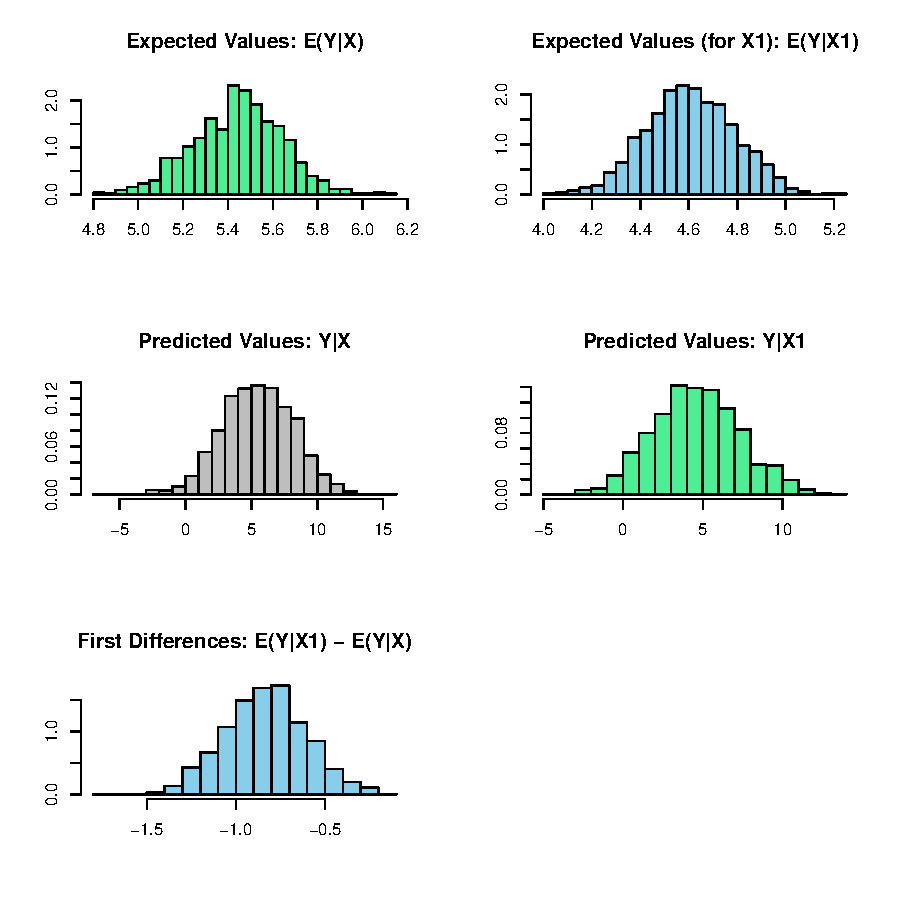
\includegraphics{vigpics/normal-ExamplesPlot}
\end{center}

\item Using Dummy Variables
%the code in this section does not work well but there is no demo for this part either
 
Estimate a model with a dummy variable for each year and country (see
\ref{factors} for help with dummy variables).  Note that you do not
need to create dummy variables, as the program will automatically
parse the unique values in the selected variables into dummy
variables.    
\begin{Schunk}
\begin{Sinput}
> z.out2 <- zelig(unem ~ gdp + trade + capmob + as.factor(year) + 
+     as.factor(country), model = "normal", data = macro)
\end{Sinput}
\end{Schunk}
Set values for the explanatory variables, using the default mean/mode
variables, with country set to the United States and Japan,
respectively: 
Simulate quantities of interest:  
%plot does not work 
\begin{center}
\end{center}
\end{enumerate}

\subsubsection{Model}
Let $Y_i$ be the continuous dependent variable for observation $i$.
\begin{itemize}
\item The \emph{stochastic component} is described by a univariate normal
  model with a vector of means $\mu_i$ and scalar variance $\sigma^2$:
  \begin{equation*}
    Y_i \; \sim \; \textrm{Normal}(\mu_i, \sigma^2). 
  \end{equation*}

\item The \emph{systematic component} is 
  \begin{equation*}
    \mu_i \;= \; x_i \beta,
  \end{equation*}
  where $x_i$ is the vector of $k$ explanatory variables and $\beta$ is
  the vector of coefficients.
\end{itemize}


\subsubsection{Quantities of Interest}

\begin{itemize}
\item The expected value ({\tt qi\$ev}) is the mean of simulations
  from the the stochastic component, $$E(Y) = \mu_i = x_i \beta,$$
  given a draw of $\beta$ from its posterior.  

\item The predicted value ({\tt qi\$pr}) is drawn from the distribution
  defined by the set of parameters $(\mu_i, \sigma)$.  

\item The first difference ({\tt qi\$fd}) is:
\begin{equation*}
\textrm{FD}\; = \;E(Y \mid x_1) -  E(Y \mid x)
\end{equation*}

\item In conditional prediction models, the average expected treatment
  effect ({\tt att.ev}) for the treatment group is 
    \begin{equation*} \frac{1}{\sum_{i=1}^n t_i}\sum_{i:t_i=1}^n \left\{ Y_i(t_i=1) -
      E[Y_i(t_i=0)] \right\},
    \end{equation*} 
    where $t_i$ is a binary explanatory variable defining the treatment
    ($t_i=1$) and control ($t_i=0$) groups.  Variation in the
    simulations are due to uncertainty in simulating $E[Y_i(t_i=0)]$,
    the counterfactual expected value of $Y_i$ for observations in the
    treatment group, under the assumption that everything stays the
    same except that the treatment indicator is switched to $t_i=0$.

\item In conditional prediction models, the average predicted treatment
  effect ({\tt att.pr}) for the treatment group is 
    \begin{equation*} \frac{1}{\sum_{i=1}^n t_i}\sum_{i:t_i=1}^n \left\{ Y_i(t_i=1) -
      \widehat{Y_i(t_i=0)} \right\},
    \end{equation*} 
    where $t_i$ is a binary explanatory variable defining the
    treatment ($t_i=1$) and control ($t_i=0$) groups.  Variation in
    the simulations are due to uncertainty in simulating
    $\widehat{Y_i(t_i=0)}$, the counterfactual predicted value of
    $Y_i$ for observations in the treatment group, under the
    assumption that everything stays the same except that the
    treatment indicator is switched to $t_i=0$.

\end{itemize}

\subsubsection{Output Values}

The output of each Zelig command contains useful information which you
may view.  For example, if you run \texttt{z.out <- zelig(y \~\,
  x, model = "normal", data)}, then you may examine the available
information in \texttt{z.out} by using \texttt{names(z.out)},
see the {\tt coefficients} by using {\tt z.out\$coefficients}, and
a default summary of information through \texttt{summary(z.out)}.
Other elements available through the {\tt \$} operator are listed
below.

\begin{itemize}
\item From the {\tt zelig()} output object {\tt z.out}, you may extract:
   \begin{itemize}
   \item {\tt coefficients}: parameter estimates for the explanatory
     variables.
   \item {\tt residuals}: the working residuals in the final iteration
     of the IWLS fit.
   \item {\tt fitted.values}: fitted values.  For the normal model,
     these are identical to the {\tt linear predictors}.
   \item {\tt linear.predictors}: fitted values.  For the normal
     model, these are identical to {\tt fitted.values}.
   \item {\tt aic}: Akaike's Information Criterion (minus twice the
     maximized log-likelihood plus twice the number of coefficients).
   \item {\tt df.residual}: the residual degrees of freedom.
   \item {\tt df.null}: the residual degrees of freedom for the null
     model.
   \item {\tt zelig.data}: the input data frame if {\tt save.data = TRUE}.  
   \end{itemize}

\item From {\tt summary(z.out)}, you may extract: 
   \begin{itemize}
   \item {\tt coefficients}: the parameter estimates with their
     associated standard errors, $p$-values, and $t$-statistics.
   \item{\tt cov.scaled}: a $k \times k$ matrix of scaled covariances.
   \item{\tt cov.unscaled}: a $k \times k$ matrix of unscaled
     covariances.  
   \end{itemize}

\item From the {\tt sim()} output object {\tt s.out}, you may extract
  quantities of interest arranged as matrices indexed by simulation
  $\times$ {\tt x}-observation (for more than one {\tt x}-observation).
  Available quantities are:

   \begin{itemize}
   \item {\tt qi\$ev}: the simulated expected values for the specified
     values of {\tt x}.
   \item {\tt qi\$pr}: the simulated predicted values drawn from the
     distribution defined by $(\mu_i, \sigma)$.
   \item {\tt qi\$fd}: the simulated first difference in the simulated
     expected values for the values specified in {\tt x} and {\tt x1}.
   \item {\tt qi\$att.ev}: the simulated average expected treatment
     effect for the treated from conditional prediction models.  
   \item {\tt qi\$att.pr}: the simulated average predicted treatment
     effect for the treated from conditional prediction models.  
   \end{itemize}
\end{itemize}

\subsection* {How to Cite} 

How to cite this model in Zelig:
\begin{verse}
  Kosuke Imai, Gary King, and Olivia Lau. 2008. "normal: Normal Regression for Continuous Dependent Variables" in Kosuke Imai, Gary King, and Olivia Lau, "Zelig: Everyone's Statistical Software,"http://gking.harvard.edu/zelig
\end{verse}

\CiteZelig

\subsection* {See also}

The normal model is part of the stats package by \citet{VenRip02}.
Advanced users may wish to refer to \texttt{help(glm)} and
\texttt{help(family)}, as well as \cite{McCNel89}. Robust standard
errors are implemented via the sandwich package by \citet{Zeileis04}.
Sample data are from \cite{KinTomWit00}.

\bibliographystyle{asa}
\bibliography{gk,gkpubs}
 



\chapter{Least Squares Regression for Continuous Dependent Variables}

\nobibliography*



\section{{\tt ls}: Least Squares Regression for Continuous
Dependent Variables}
\label{ls}

Use least squares regression analysis to estimate the best linear
predictor for the specified dependent variables.

\subsubsection{Syntax}

\begin{verbatim}
> z.out <- zelig(Y ~ X1 + X2, model = "ls", data = mydata)
> x.out <- setx(z.out)
> s.out <- sim(z.out, x = x.out)
\end{verbatim}

\subsubsection{Additional Inputs}  

In addition to the standard inputs, {\tt zelig()} takes the following
additional options for least squares regression:  
\begin{itemize}
\item {\tt robust}: defaults to {\tt FALSE}.  If {\tt TRUE} is
selected, {\tt zelig()} computes robust standard errors based on
sandwich estimators (see \cite{Zeileis04}, \cite{Huber81}, and
\cite{White80}).  The default type of robust standard error is
heteroskedastic consistent (HC), \emph{not} heteroskedastic and
autocorrelation consistent (HAC).  

In addition, {\tt robust} may be a list with the following options:  
\begin{itemize}
\item {\tt method}:  choose from 
\begin{itemize}
\item {\tt "vcovHC"}: (the default if {\tt robust = TRUE}), HC standard errors.
\item {\tt "vcovHAC"}: HAC standard errors without weights.  
\item {\tt "kernHAC"}: HAC standard errors using the weights given in
\cite{Andrews91}.   
\item {\tt "weave"}: HAC standard errors using the weights given in
\cite{LumHea99}.
\end{itemize} 
\item {\tt order.by}: only applies to the HAC methods above.  Defaults to
{\tt NULL} (the observations are chronologically ordered as in the
original data).  Optionally, you may specify a time index (either as
{\tt order.by = z}, where {\tt z} exists outside the data frame; or
as {\tt order.by = \~{}z}, where {\tt z} is a variable in the data
frame).  The observations are chronologically ordered by the size of
{\tt z}.
\item {\tt \dots}:  additional options passed to the functions
specified in {\tt method}.  See the {\tt sandwich} library and
\cite{Zeileis04} for more options.   
\end{itemize}
\end{itemize}

\subsubsection{Examples}\begin{enumerate}
\item Basic Example with First Differences

Attach sample data:
\begin{Schunk}
\begin{Sinput}
> data(macro)
\end{Sinput}
\end{Schunk}
Estimate model:
\begin{Schunk}
\begin{Sinput}
> z.out1 <- zelig(unem ~ gdp + capmob + trade, model = "ls", data = macro)
\end{Sinput}
\end{Schunk}
Summarize regression coefficients:
\begin{Schunk}
\begin{Sinput}
> summary(z.out1)
\end{Sinput}
\end{Schunk}
Set explanatory variables to their default (mean/mode) values, with
high (80th percentile) and low (20th percentile) values for the trade variable:
\begin{Schunk}
\begin{Sinput}
> x.high <- setx(z.out1, trade = quantile(macro$trade, 0.8))
> x.low <- setx(z.out1, trade = quantile(macro$trade, 0.2))
\end{Sinput}
\end{Schunk}
Generate first differences for the effect of high versus low trade on
GDP:
\begin{Schunk}
\begin{Sinput}
> s.out1 <- sim(z.out1, x = x.high, x1 = x.low)
\end{Sinput}
\end{Schunk}
\begin{Schunk}
\begin{Sinput}
> summary(s.out1)
\end{Sinput}
\end{Schunk}
\begin{center}
\begin{Schunk}
\begin{Sinput}
> plot(s.out1)
\end{Sinput}
\end{Schunk}
\includegraphics{vigpics/gamma-ExamplesPlot}
\end{center}

\item Using Dummy Variables

Estimate a model with fixed effects for each country (see
\Sref{factors} for help with dummy variables).  Note that you do not
need to create dummy variables, as the program will automatically
parse the unique values in the selected variable into discrete levels.  
\begin{Schunk}
\begin{Sinput}
> z.out2 <- zelig(unem ~ gdp + trade + capmob + as.factor(country), 
+     model = "ls", data = macro)
\end{Sinput}
\end{Schunk}
Set values for the explanatory variables, using the default mean/mode
values, with country set to the United States and Japan, respectively:
\begin{Schunk}
\begin{Sinput}
> x.US <- setx(z.out2, country = "United States")
> x.Japan <- setx(z.out2, country = "Japan")
\end{Sinput}
\end{Schunk}
Simulate quantities of interest:
\begin{Schunk}
\begin{Sinput}
> s.out2 <- sim(z.out2, x = x.US, x1 = x.Japan)
\end{Sinput}
\end{Schunk}
\begin{center}
\begin{Schunk}
\begin{Sinput}
> plot(s.out2)
\end{Sinput}
\end{Schunk}
\includegraphics{vigpics/gamma-DummyPlot}
\end{center}

% \item Multiple responses (least squares regression will be fitted
%   separately to each dependent variable)

% Two responses for data set macro: 
% <<Multiple.zelig>>=
%  z.out3 <- zelig(cbind(unem, gdp) ~ capmob + trade,model = "ls", data = macro)
% @
% <<Multiple.zelig.summary>>=
% summary(z.out3)
% @    
% Set values for the explanatory variables, using the default mean/mode
% values, with country set to the United States and Japan, respectively:
% <<Multiple.setx>>=
%  x.US <- setx(z.out3, country = "United States")
%  x.Japan <- setx(z.out3, country = "Japan")
% @ 
% Simulate quantities of interest:
% <<Multiple.sim>>=
%  s.out3 <- sim(z.out3, x = x.US, x1 = x.Japan)
% @
% Summary
% <<Example4.sim.summary>>=
% summary(s.out3)
% @  
% \begin{center}
% <<label=Example4Plot,fig=true,echo=true,  width=7.5, height=6>>= 
%  plot(s.out3)
% @ 
\end{center}

\end{enumerate}

\subsubsection{Model}
\begin{itemize}
\item The \emph{stochastic component} is described by a density
  with mean $\mu_i$ and the common variance $\sigma^2$
  \begin{equation*}
    Y_i \; \sim \; f(y_i \mid \mu_i, \sigma^2).
  \end{equation*}
\item The \emph{systematic component} models the conditional mean as
  \begin{equation*}
     \mu_i =  x_i \beta
  \end{equation*} 
  where $x_i$ is the vector of covariates, and $\beta$ is the vector
  of coefficients.
  
  The least squares estimator is the best linear predictor of a
  dependent variable given $x_i$, and minimizes the sum of squared
  residuals, $\sum_{i=1}^n (Y_i-x_i \beta)^2$.  
\end{itemize}

\subsubsection{Quantities of Interest} 
\begin{itemize}
\item The expected value ({\tt qi\$ev}) is the mean of simulations
  from the stochastic component,  
\begin{equation*}
E(Y) = x_i \beta,\end{equation*}
given a draw of $\beta$ from its sampling distribution.  

\item In conditional prediction models, the average expected treatment
  effect ({\tt att.ev}) for the treatment group is 
    \begin{equation*} \frac{1}{\sum_{i=1}^n t_i}\sum_{i:t_i=1}^n \left\{ Y_i(t_i=1) -
      E[Y_i(t_i=0)] \right\},
    \end{equation*} 
    where $t_i$ is a binary explanatory variable defining the treatment
    ($t_i=1$) and control ($t_i=0$) groups.  Variation in the
    simulations are due to uncertainty in simulating $E[Y_i(t_i=0)]$,
    the counterfactual expected value of $Y_i$ for observations in the
    treatment group, under the assumption that everything stays the
    same except that the treatment indicator is switched to $t_i=0$.

\end{itemize}

\subsubsection{Output Values}

The output of each Zelig command contains useful information which you
may view.  For example, if you run \texttt{z.out <- zelig(y \~\,
  x, model = "ls", data)}, then you may examine the available
information in \texttt{z.out} by using \texttt{names(z.out)},
see the {\tt coefficients} by using {\tt z.out\$coefficients}, and
a default summary of information through \texttt{summary(z.out)}.
Other elements available through the {\tt \$} operator are listed
below.

\begin{itemize}
  \item From the {\tt zelig()} output object {\tt z.out}, you may
  extract:
   \begin{itemize}
   \item {\tt coefficients}: parameter estimates for the explanatory
     variables.
   \item {\tt residuals}: the working residuals in the final iteration
     of the IWLS fit.
   \item {\tt fitted.values}: fitted values.
   \item {\tt df.residual}: the residual degrees of freedom.
   \item {\tt zelig.data}: the input data frame if {\tt save.data = TRUE}.  
   \end{itemize}
  
\item From {\tt summary(z.out)}, you may extract:
   \begin{itemize}
   \item {\tt coefficients}: the parameter estimates with their
     associated standard errors, $p$-values, and $t$-statistics.
     \begin{equation*}
       \hat{\beta} \; = \; \left(\sum_{i=1}^n x_i' x_i\right)^{-1} \sum x_i y_i
     \end{equation*}
   \item {\tt sigma}: the square root of the estimate variance of the
     random error $e$:
     \begin{equation*}
       \hat{\sigma} \; = \; \frac{\sum (Y_i-x_i\hat{\beta})^2}{n-k}
     \end{equation*}
   \item {\tt r.squared}: the fraction of the variance explained by
     the model. 
     \begin{equation*}
       R^2 \; = \; 1 - \frac{\sum (Y_i-x_i\hat{\beta})^2}{\sum (y_i -
         \bar{y})^2} 
     \end{equation*}
   \item {\tt adj.r.squared}: the above $R^2$ statistic, penalizing
     for an increased number of explanatory variables.  
   \item{\tt cov.unscaled}: a $k \times k$ matrix of unscaled
     covariances.  
   \end{itemize}
   
\item From the {\tt sim()} output object {\tt s.out}, you may extract
  quantities of interest arranged as matrices indexed by simulation
  $\times$ {\tt x}-observation (for more than one {\tt x}-observation).
  Available quantities are:

   \begin{itemize}
   \item {\tt qi\$ev}: the simulated expected values for the specified
     values of {\tt x}.
   \item {\tt qi\$fd}:  the simulated first differences (or
     differences in expected values) for the specified values of {\tt
       x} and {\tt x1}. 
   \item {\tt qi\$att.ev}: the simulated average expected treatment
     effect for the treated from conditional prediction models.  
   \end{itemize}
\end{itemize}

\subsection* {How to Cite} 


How to cite this model in Zelig:
\begin{verse}
  Kosuke Imai, Gary King, and Olivia Lau. 2007. "ls: Least Squares Regression for Continuous Dependent Variables" in Kosuke Imai, Gary King, and Olivia Lau, "Zelig: Everyone's Statistical Software,"http://gking.harvard.edu/zelig
\end{verse}

\CiteZelig

\subsection* {See also}
The least squares regression is part of the stats package by William N.
Venables and Brian D. Ripley \citep{VenRip02}.In addition, advanced users may wish to refer to \texttt{help(lm)} and \texttt{help(lm.fit)}.Robust standard errors are implemented via the sandwich package by Achim Zeileis \citep{Zeileis04}.Sample data are from \cite{KinTomWit00}.

\bibliographystyle{asa}
\bibliography{gk,gkpubs}
 



\chapter{Gamma Regression for Continuous, Positive Dependent Variables}

\nobibliography*


\section{{\tt gamma}: Gamma Regression for Continuous, Positive Dependent Variables}\label{gamma}

Use the gamma regression model if you have a positive-valued dependent
variable such as the number of years a parliamentary cabinet endures,
or the seconds you can stay airborne while jumping.  The gamma
distribution assumes that all waiting times are complete by the end
of the study (censoring is not allowed).

\subsubsection{Syntax}

\begin{verbatim}
> z.out <- zelig(Y ~ X1 + X2, model = "gamma", data = mydata)
> x.out <- setx(z.out)
> s.out <- sim(z.out, x = x.out, x1 = NULL)
\end{verbatim}

\subsubsection{Additional Inputs} 

In addition to the standard inputs, {\tt zelig()} takes the following
additional options for gamma regression:  
\begin{itemize}
\item {\tt robust}: defaults to {\tt FALSE}.  If {\tt TRUE} is
selected, {\tt zelig()} computes robust standard errors via the {\tt
sandwich} package (see \cite{Zeileis04}).  The default type of robust
standard error is heteroskedastic and autocorrelation consistent (HAC),
and assumes that observations are ordered by time index.

In addition, {\tt robust} may be a list with the following options:  
\begin{itemize}
\item {\tt method}:  Choose from 
\begin{itemize}
\item {\tt "vcovHAC"}: (default if {\tt robust = TRUE}) HAC standard
errors. 
\item {\tt "kernHAC"}: HAC standard errors using the
weights given in \cite{Andrews91}. 
\item {\tt "weave"}: HAC standard errors using the
weights given in \cite{LumHea99}.  
\end{itemize}  
\item {\tt order.by}: defaults to {\tt NULL} (the observations are
chronologically ordered as in the original data).  Optionally, you may
specify a vector of weights (either as {\tt order.by = z}, where {\tt
z} exists outside the data frame; or as {\tt order.by = \~{}z}, where
{\tt z} is a variable in the data frame).  The observations are
chronologically ordered by the size of {\tt z}.
\item {\tt \dots}:  additional options passed to the functions 
specified in {\tt method}.   See the {\tt sandwich} library and
\cite{Zeileis04} for more options.   
\end{itemize}
\end{itemize}

\subsubsection{Example}

Attach the sample data: 
\begin{Schunk}
\begin{Sinput}
> data(coalition)
\end{Sinput}
\end{Schunk}
Estimate the model: 
\begin{Schunk}
\begin{Sinput}
> z.out <- zelig(duration ~ fract + numst2, model = "gamma", data = coalition)
\end{Sinput}
\end{Schunk}
View the regression output:  
\begin{Schunk}
\begin{Sinput}
> summary(z.out)
\end{Sinput}
\end{Schunk}
Set the baseline values (with the ruling coalition in the minority)
and the alternative values (with the ruling coalition in the majority)
for X:
\begin{Schunk}
\begin{Sinput}
> x.low <- setx(z.out, numst2 = 0)
> x.high <- setx(z.out, numst2 = 1)
\end{Sinput}
\end{Schunk}
Simulate expected values ({\tt qi\$ev}) and first differences ({\tt qi\$fd}):
\begin{Schunk}
\begin{Sinput}
> s.out <- sim(z.out, x = x.low, x1 = x.high)
\end{Sinput}
\end{Schunk}
\begin{Schunk}
\begin{Sinput}
> summary(s.out)
\end{Sinput}
\end{Schunk}
\begin{center}
\begin{Schunk}
\begin{Sinput}
> plot(s.out)
\end{Sinput}
\end{Schunk}
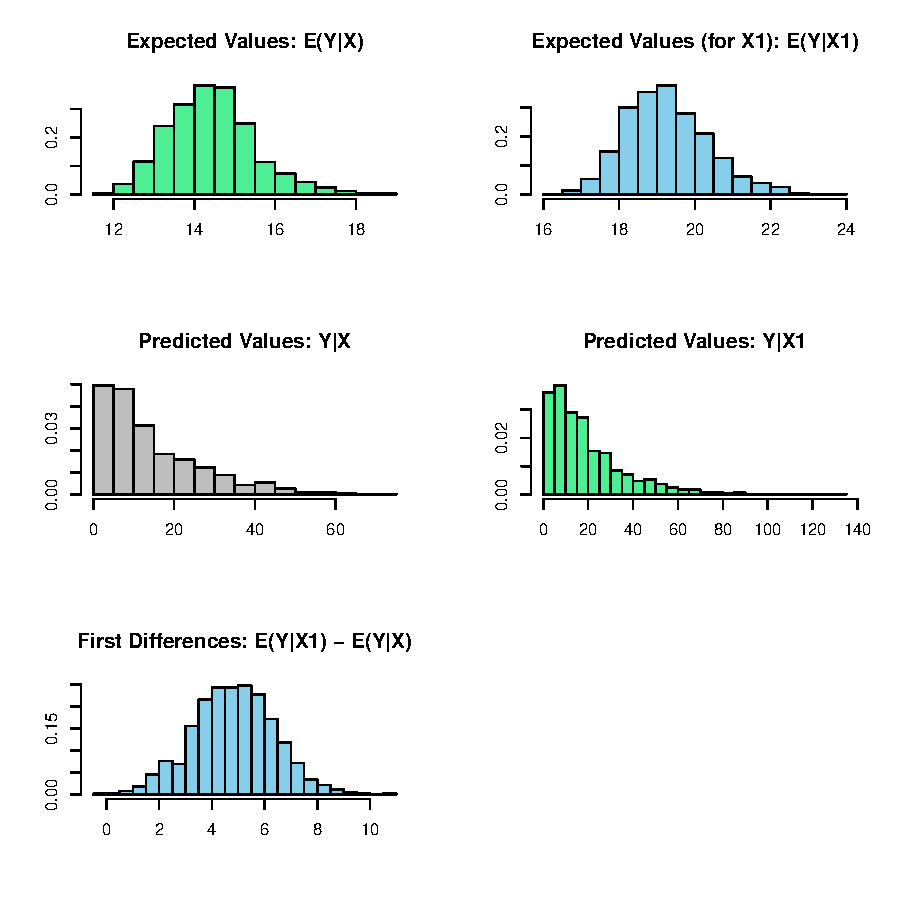
\includegraphics{vigpics/gamma-ExamplePlot}
\end{center}

\subsubsection{Model}

\begin{itemize}
\item The Gamma distribution with scale parameter $\alpha$ has a
\emph{stochastic component}:
\begin{eqnarray*}
Y &\sim& \textrm{Gamma}(y_i \mid \lambda_i, \alpha) \\
f(y)  &=& \frac{1}{\alpha^{\lambda_i} \, \Gamma \lambda_i} \, y_i^{\lambda_i
  - 1} \exp -\left\{ \frac{y_i}{\alpha} \right\}
\end{eqnarray*}
for $\alpha, \lambda_i, y_i > 0$.  \\

\item The \emph{systematic component} is given by
\begin{equation*}
  \lambda_i = \frac{1}{x_i \beta}
\end{equation*}
\end{itemize}

\subsubsection{Quantities of Interest}

\begin{itemize}
\item The expected values ({\tt qi\$ev}) are simulations of the mean
  of the stochastic component given draws of $\alpha$ and
  $\beta$ from their posteriors:  $$E(Y) = \alpha \lambda_i.$$  
\item The predicted values ({\tt qi\$pr}) are draws from the gamma
  distribution for each given set of parameters $(\alpha, \lambda_i)$.
\item If {\tt x1} is specified, {\tt sim()} also returns the
  differences in the expected values ({\tt qi\$fd}), $$E(Y \mid x_1) -
  E(Y \mid x)$$.

\item In conditional prediction models, the average expected treatment
  effect ({\tt att.ev}) for the treatment group is 
    \begin{equation*} \frac{1}{\sum_{i=1}^n t_i}\sum_{i:t_i=1}^n \left\{ Y_i(t_i=1) -
      E[Y_i(t_i=0)] \right\},
    \end{equation*} 
    where $t_i$ is a binary explanatory variable defining the treatment
    ($t_i=1$) and control ($t_i=0$) groups.  Variation in the
    simulations are due to uncertainty in simulating $E[Y_i(t_i=0)]$,
    the counterfactual expected value of $Y_i$ for observations in the
    treatment group, under the assumption that everything stays the
    same except that the treatment indicator is switched to $t_i=0$.

\item In conditional prediction models, the average predicted treatment
  effect ({\tt att.pr}) for the treatment group is 
    \begin{equation*} \frac{1}{\sum_{i=1}^n t_i}\sum_{i:t_i=1}^n \left\{ Y_i(t_i=1) -
      \widehat{Y_i(t_i=0)} \right\},
    \end{equation*} 
    where $t_i$ is a binary explanatory variable defining the treatment
    ($t_i=1$) and control ($t_i=0$) groups.  Variation in the
    simulations are due to uncertainty in simulating
    $\widehat{Y_i(t_i=0)}$, the counterfactual predicted value of
    $Y_i$ for observations in the treatment group, under the
    assumption that everything stays the same except that the
    treatment indicator is switched to $t_i=0$.  

\end{itemize}

\subsubsection{Output Values}

The output of each Zelig command contains useful information which you
may view.  For example, if you run \texttt{z.out <- zelig(y \~\,
  x, model = "gamma", data)}, then you may examine the available
information in \texttt{z.out} by using \texttt{names(z.out)},
see the {\tt coefficients} by using {\tt z.out\$coefficients}, and
a default summary of information through \texttt{summary(z.out)}.
Other elements available through the {\tt \$} operator are listed
below.

\begin{itemize}
\item From the {\tt zelig()} output object {\tt z.out}, you may
  extract:
   \begin{itemize}
   \item {\tt coefficients}: parameter estimates for the explanatory
     variables.
   \item {\tt residuals}: the working residuals in the final iteration
     of the IWLS fit.
   \item {\tt fitted.values}: the vector of fitted values.
   \item {\tt linear.predictors}: the vector of $x_{i}\beta$.
   \item {\tt aic}: Akaike's Information Criterion (minus twice the
     maximized log-likelihood plus twice the number of coefficients).
   \item {\tt df.residual}: the residual degrees of freedom.
   \item {\tt df.null}: the residual degrees of freedom for the null
     model.
   \item {\tt zelig.data}: the input data frame if {\tt save.data = TRUE}.  
   \end{itemize}

\item From {\tt summary(z.out)}, you may extract: 
   \begin{itemize}
   \item {\tt coefficients}: the parameter estimates with their
     associated standard errors, $p$-values, and $t$-statistics.
   \item{\tt cov.scaled}: a $k \times k$ matrix of scaled covariances.
   \item{\tt cov.unscaled}: a $k \times k$ matrix of unscaled
     covariances.  
   \end{itemize}

\item From the {\tt sim()} output object {\tt s.out}, you may extract
  quantities of interest arranged as matrices indexed by simulation
  $\times$ {\tt x}-observation (for more than one {\tt x}-observation).
  Available quantities are:

   \begin{itemize}
   \item {\tt qi\$ev}: the simulated expected values for the specified
     values of {\tt x}.
   \item {\tt qi\$pr}: the simulated predicted values drawn from a
     distribution defined by $(\alpha, \lambda_i)$.
   \item {\tt qi\$fd}: the simulated first difference in the expected
     values for the specified values in {\tt x} and {\tt x1}.
   \item {\tt qi\$att.ev}: the simulated average expected treatment
     effect for the treated from conditional prediction models.  
   \item {\tt qi\$att.pr}: the simulated average predicted treatment
     effect for the treated from conditional prediction models.  
   \end{itemize}
\end{itemize}


\subsection* {How to Cite} 


How to cite this model in Zelig:
\begin{verse}
  Kosuke Imai, Gary King, and Olivia Lau. 2007. "gamma: Gamma Regression for Continuous, Positive Dependent Variables" in Kosuke Imai, Gary King, and Olivia Lau, "Zelig: Everyone's Statistical Software,"http://gking.harvard.edu/zelig
\end{verse}

\CiteZelig 

\subsection* {See also}
The gamma model is part of the stats package by \citet{VenRip02}.
Advanced users may wish to refer to \texttt{help(glm)} and
\texttt{help(family)}, as well as \cite{McCNel89}. Robust standard
verrors are implemented via the sandwich package by \citet{Zeileis04}.
Sample data are from \cite{KinTomWit00}.

\bibliographystyle{asa}
\bibliography{gk,gkpubs}




\chapter{Poisson Regression for Event Count Dependent Variables}

\nobibliography*


\section{{\tt poisson}: Poisson Regression for Event Count
Dependent Variables}\label{poisson}

Use the Poisson regression model if the observations of your dependent
variable represents the number of independent events that occur during
a fixed period of time (see the negative binomial model, \Sref{negbin},
for over-dispersed event counts.)  For a Bayesian implementation of
this model, see \Sref{poisson.bayes}.  

\subsubsection{Syntax}

\begin{verbatim}
> z.out <- zelig(Y ~ X1 + X2, model = "poisson", data = mydata)
> x.out <- setx(z.out)
> s.out <- sim(z.out, x = x.out)
\end{verbatim}

\subsubsection{Additional Inputs} 

In addition to the standard inputs, {\tt zelig()} takes the following
additional options for poisson regression:  
\begin{itemize}
\item {\tt robust}: defaults to {\tt FALSE}.  If {\tt TRUE} is
selected, {\tt zelig()} computes robust standard errors via the {\tt
sandwich} package (see \cite{Zeileis04}).  The default type of robust
standard error is heteroskedastic and autocorrelation consistent (HAC),
and assumes that observations are ordered by time index.

In addition, {\tt robust} may be a list with the following options:  
\begin{itemize}
\item {\tt method}:  Choose from 
\begin{itemize}
\item {\tt "vcovHAC"}: (default if {\tt robust = TRUE}) HAC standard
errors. 
\item {\tt "kernHAC"}: HAC standard errors using the
weights given in \cite{Andrews91}. 
\item {\tt "weave"}: HAC standard errors using the
weights given in \cite{LumHea99}.  
\end{itemize}  
\item {\tt order.by}: defaults to {\tt NULL} (the observations are
chronologically ordered as in the original data).  Optionally, you may
specify a vector of weights (either as {\tt order.by = z}, where {\tt
z} exists outside the data frame; or as {\tt order.by = \~{}z}, where
{\tt z} is a variable in the data frame).  The observations are
chronologically ordered by the size of {\tt z}.
\item {\tt \dots}:  additional options passed to the functions 
specified in {\tt method}.   See the {\tt sandwich} library and
\cite{Zeileis04} for more options.   
\end{itemize}
\end{itemize}

\subsubsection{Example}

Load sample data:  
\begin{Schunk}
\begin{Sinput}
> data(sanction)
\end{Sinput}
\end{Schunk}
Estimate Poisson model:  
\begin{Schunk}
\begin{Sinput}
> z.out <- zelig(num ~ target + coop, model = "poisson", data = sanction)
\end{Sinput}
\end{Schunk}
\begin{Schunk}
\begin{Sinput}
> summary(z.out)
\end{Sinput}
\end{Schunk}
Set values for the explanatory variables to their default mean values:  
\begin{Schunk}
\begin{Sinput}
> x.out <- setx(z.out)
\end{Sinput}
\end{Schunk}
Simulate fitted values:  
\begin{Schunk}
\begin{Sinput}
> s.out <- sim(z.out, x = x.out)
\end{Sinput}
\end{Schunk}
\begin{Schunk}
\begin{Sinput}
> summary(s.out)
\end{Sinput}
\end{Schunk}
\begin{center}
\begin{Schunk}
\begin{Sinput}
> plot(s.out)
\end{Sinput}
\end{Schunk}
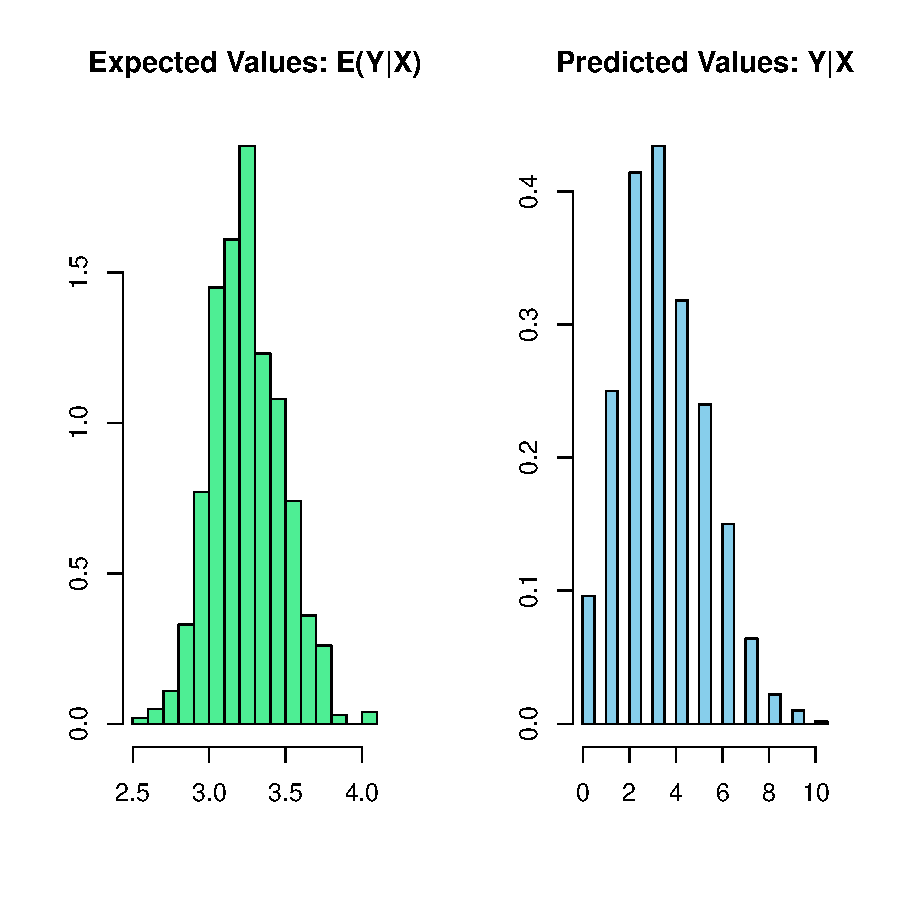
\includegraphics{vigpics/poisson-ExamplePlot}
\end{center}

\subsubsection{Model}
Let $Y_i$ be the number of independent events that occur during a
fixed time period. This variable can take any non-negative integer.

\begin{itemize}
\item The Poisson distribution has \emph{stochastic component}
  \begin{equation*}
    Y_i \; \sim \; \textrm{Poisson}(\lambda_i),
  \end{equation*}
  where $\lambda_i$ is the mean and variance parameter.
  
\item The \emph{systematic component} is 
  \begin{equation*}
    \lambda_i \; = \; \exp(x_i \beta),
  \end{equation*}
  where $x_i$ is the vector of explanatory variables, and $\beta$ is
  the vector of coefficients.
\end{itemize}

\subsubsection{Quantities of Interest}

\begin{itemize}
  
\item The expected value ({\tt qi\$ev}) is the mean of simulations
  from the stochastic component, $$E(Y) = \lambda_i =  \exp(x_i
  \beta),$$ given draws of $\beta$ from its sampling distribution.  
  
\item The predicted value ({\tt qi\$pr}) is a random draw from the
  poisson distribution defined by mean $\lambda_i$.

\item The first difference in the expected values ({\tt qi\$fd}) is given by:
\begin{equation*}
\textrm{FD} \; = \; E(Y | x_1) - E(Y \mid x)
\end{equation*}
\item In conditional prediction models, the average expected treatment
  effect ({\tt att.ev}) for the treatment group is 
    \begin{equation*} \frac{1}{\sum_{i=1}^n t_i}\sum_{i:t_i=1}^n \left\{ Y_i(t_i=1) -
      E[Y_i(t_i=0)] \right\},
    \end{equation*} 
    where $t_i$ is a binary explanatory variable defining the treatment
    ($t_i=1$) and control ($t_i=0$) groups.  Variation in the
    simulations are due to uncertainty in simulating $E[Y_i(t_i=0)]$,
    the counterfactual expected value of $Y_i$ for observations in the
    treatment group, under the assumption that everything stays the
    same except that the treatment indicator is switched to $t_i=0$.

\item In conditional prediction models, the average predicted treatment
  effect ({\tt att.pr}) for the treatment group is 
    \begin{equation*} \frac{1}{\sum_{i=1}^n t_i}\sum_{i:t_i=1}^n \left\{ Y_i(t_i=1) -
      \widehat{Y_i(t_i=0)} \right\},
    \end{equation*} 
    where $t_i$ is a binary explanatory variable defining the
    treatment ($t_i=1$) and control ($t_i=0$) groups.  Variation in
    the simulations are due to uncertainty in simulating
    $\widehat{Y_i(t_i=0)}$, the counterfactual predicted value of
    $Y_i$ for observations in the treatment group, under the
    assumption that everything stays the same except that the
    treatment indicator is switched to $t_i=0$.
\end{itemize}

\subsubsection{Output Values}

The output of each Zelig command contains useful information which you
may view.  For example, if you run \texttt{z.out <- zelig(y \~\,
  x, model = "poisson", data)}, then you may examine the available
information in \texttt{z.out} by using \texttt{names(z.out)},
see the {\tt coefficients} by using {\tt z.out\$coefficients}, and
a default summary of information through \texttt{summary(z.out)}.
Other elements available through the {\tt \$} operator are listed
below.

\begin{itemize}
\item From the {\tt zelig()} output object {\tt z.out}, you may extract:
   \begin{itemize}
   \item {\tt coefficients}: parameter estimates for the explanatory
     variables.
   \item {\tt residuals}: the working residuals in the final iteration
     of the IWLS fit.
   \item {\tt fitted.values}: a vector of the fitted values for the systemic
     component $\lambda$.  
   \item {\tt linear.predictors}: a vector of $x_{i}\beta$.  
   \item {\tt aic}: Akaike's Information Criterion (minus twice the
     maximized log-likelihood plus twice the number of coefficients).
   \item {\tt df.residual}: the residual degrees of freedom.
   \item {\tt df.null}: the residual degrees of freedom for the null
     model.
   \item {\tt zelig.data}: the input data frame if {\tt save.data = TRUE}.  
   \end{itemize}

\item From {\tt summary(z.out)}, you may extract: 
   \begin{itemize}
   \item {\tt coefficients}: the parameter estimates with their
     associated standard errors, $p$-values, and $t$-statistics.
   \item{\tt cov.scaled}: a $k \times k$ matrix of scaled covariances.
   \item{\tt cov.unscaled}: a $k \times k$ matrix of unscaled
     covariances.  
   \end{itemize}

\item From the {\tt sim()} output object {\tt s.out}, you may extract
  quantities of interest arranged as matrices indexed by simulation
  $\times$ {\tt x}-observation (for more than one {\tt x}-observation).
  Available quantities are:

   \begin{itemize}
   \item {\tt qi\$ev}: the simulated expected values given the
     specified values of {\tt x}.
   \item {\tt qi\$pr}: the simulated predicted values drawn from the
     distributions defined by $\lambda_i$.
   \item {\tt qi\$fd}: the simulated first differences in the expected
     values given the specified values of {\tt x} and {\tt x1}.
   \item {\tt qi\$att.ev}: the simulated average expected treatment
     effect for the treated from conditional prediction models.  
   \item {\tt qi\$att.pr}: the simulated average predicted treatment
     effect for the treated from conditional prediction models.  
   \end{itemize}
\end{itemize}

\subsection* {How to Cite} 

How to cite this model in Zelig:
\begin{verse}
  Kosuke Imai, Gary King, and Olivia Lau. 2007. "poisson: Poisson Regression for Event Count Dependent Variables" in Kosuke Imai, Gary King, and Olivia Lau, "Zelig: Everyone's Statistical Software,"http://gking.harvard.edu/zelig
\end{verse}
\CiteZelig
\subsection* {See also}
The poisson model is part of the stats package by \citet{VenRip02}.
Advanced users may wish to refer to \texttt{help(glm)} and
\texttt{help(family)}, as well as \cite{McCNel89}. Robust standard
errors are implemented via the sandwich package by \citet{Zeileis04}.
Sample data are from \cite{Martin92}.

\bibliographystyle{asa}
\bibliography{gk,gkpubs}
 



\chapter{Logistic Regression for Dichotomous Dependent Variables}

\nobibliography*


\section{{\tt logit}: Logistic Regression for Dichotomous Dependent
Variables}\label{logit}

Logistic regression specifies a dichotomous dependent variable as a
function of a set of explanatory variables.  For a Bayesian
implementation, see \Sref{logit.bayes}.  

\subsubsection{Syntax}

\begin{verbatim}
> z.out <- zelig(Y ~ X1 + X2, model = "logit", data = mydata)
> x.out <- setx(z.out)
> s.out <- sim(z.out, x = x.out, x1 = NULL)
\end{verbatim}

\subsubsection{Additional Inputs} 

In addition to the standard inputs, {\tt zelig()} takes the following
additional options for logistic regression:  
\begin{itemize}
\item {\tt robust}: defaults to {\tt FALSE}.  If {\tt TRUE} is
selected, {\tt zelig()} computes robust standard errors via the {\tt
sandwich} package (see \cite{Zeileis04}).  The default type of robust
standard error is heteroskedastic and autocorrelation consistent (HAC),
and assumes that observations are ordered by time index.

In addition, {\tt robust} may be a list with the following options:  
\begin{itemize}
\item {\tt method}:  Choose from 
\begin{itemize}
\item {\tt "vcovHAC"}: (default if {\tt robust = TRUE}) HAC standard
errors. 
\item {\tt "kernHAC"}: HAC standard errors using the
weights given in \cite{Andrews91}. 
\item {\tt "weave"}: HAC standard errors using the
weights given in \cite{LumHea99}.  
\end{itemize}  
\item {\tt order.by}: defaults to {\tt NULL} (the observations are
chronologically ordered as in the original data).  Optionally, you may
specify a vector of weights (either as {\tt order.by = z}, where {\tt
z} exists outside the data frame; or as {\tt order.by = \~{}z}, where
{\tt z} is a variable in the data frame)  The observations are
chronologically ordered by the size of {\tt z}.
\item {\tt \dots}:  additional options passed to the functions 
specified in {\tt method}.   See the {\tt sandwich} library and
\cite{Zeileis04} for more options.   
\end{itemize}
\end{itemize}

\subsubsection{Examples}
\begin{enumerate}
\item {Basic Example}
 
Attaching the sample turnout dataset:
\begin{Schunk}
\begin{Sinput}
> data(turnout)
\end{Sinput}
\end{Schunk}
Estimating parameter values for the logistic regression:
\begin{Schunk}
\begin{Sinput}
> z.out1 <- zelig(vote ~ age + race, model = "logit", data = turnout)
\end{Sinput}
\end{Schunk}
Setting values for the explanatory variables:
\begin{Schunk}
\begin{Sinput}
> x.out1 <- setx(z.out1, age = 36, race = "white")
\end{Sinput}
\end{Schunk}
Simulating quantities of interest from the posterior distribution.
\begin{Schunk}
\begin{Sinput}
> s.out1 <- sim(z.out1, x = x.out1)
\end{Sinput}
\end{Schunk}
\begin{Schunk}
\begin{Sinput}
> summary(s.out1)
\end{Sinput}
\end{Schunk}
\begin{center}
\begin{Schunk}
\begin{Sinput}
> plot(s.out1)
\end{Sinput}
\end{Schunk}
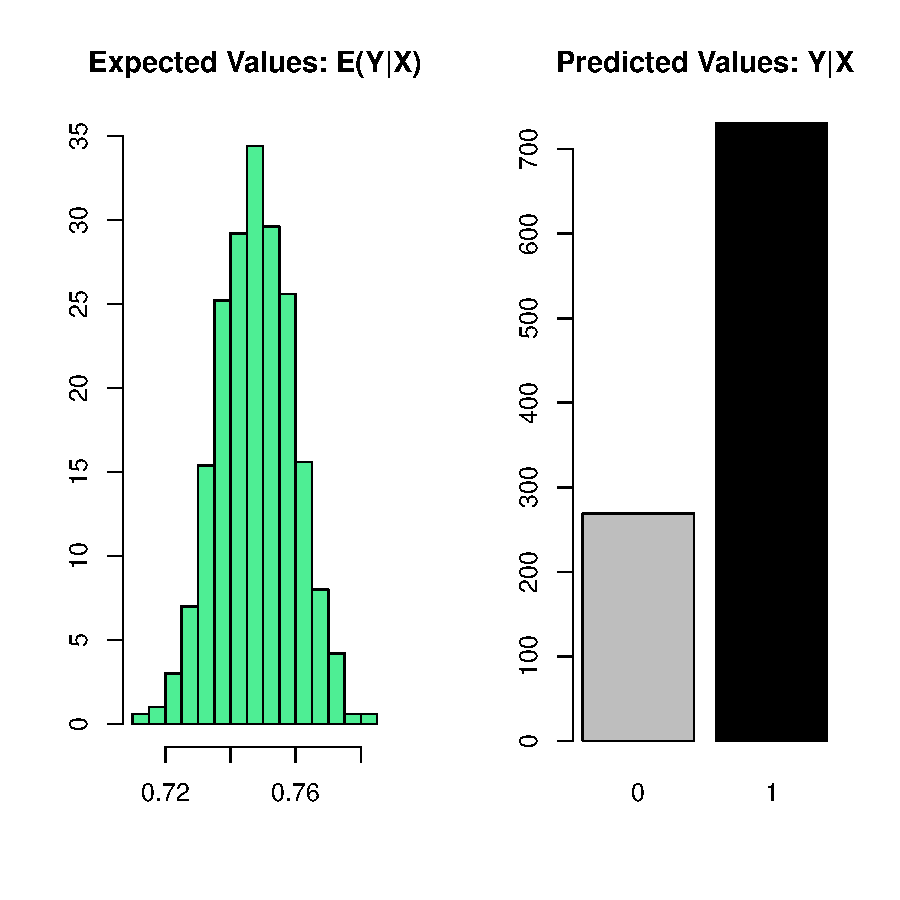
\includegraphics{vigpics/logit-ExamplePlot}
\end{center}

\item {Simulating First Differences}

Estimating the risk difference (and risk ratio) between low education
(25th percentile) and high education (75th percentile) while all the
other variables held at their default values.
\begin{Schunk}
\begin{Sinput}
> z.out2 <- zelig(vote ~ race + educate, model = "logit", data = turnout)
> x.high <- setx(z.out2, educate = quantile(turnout$educate, prob = 0.75))
> x.low <- setx(z.out2, educate = quantile(turnout$educate, prob = 0.25))
\end{Sinput}
\end{Schunk}

\begin{Schunk}
\begin{Sinput}
> s.out2 <- sim(z.out2, x = x.high, x1 = x.low)
\end{Sinput}
\end{Schunk}
\begin{Schunk}
\begin{Sinput}
> summary(s.out2)
\end{Sinput}
\end{Schunk}
\begin{center}
\begin{Schunk}
\begin{Sinput}
> plot(s.out2)
\end{Sinput}
\end{Schunk}
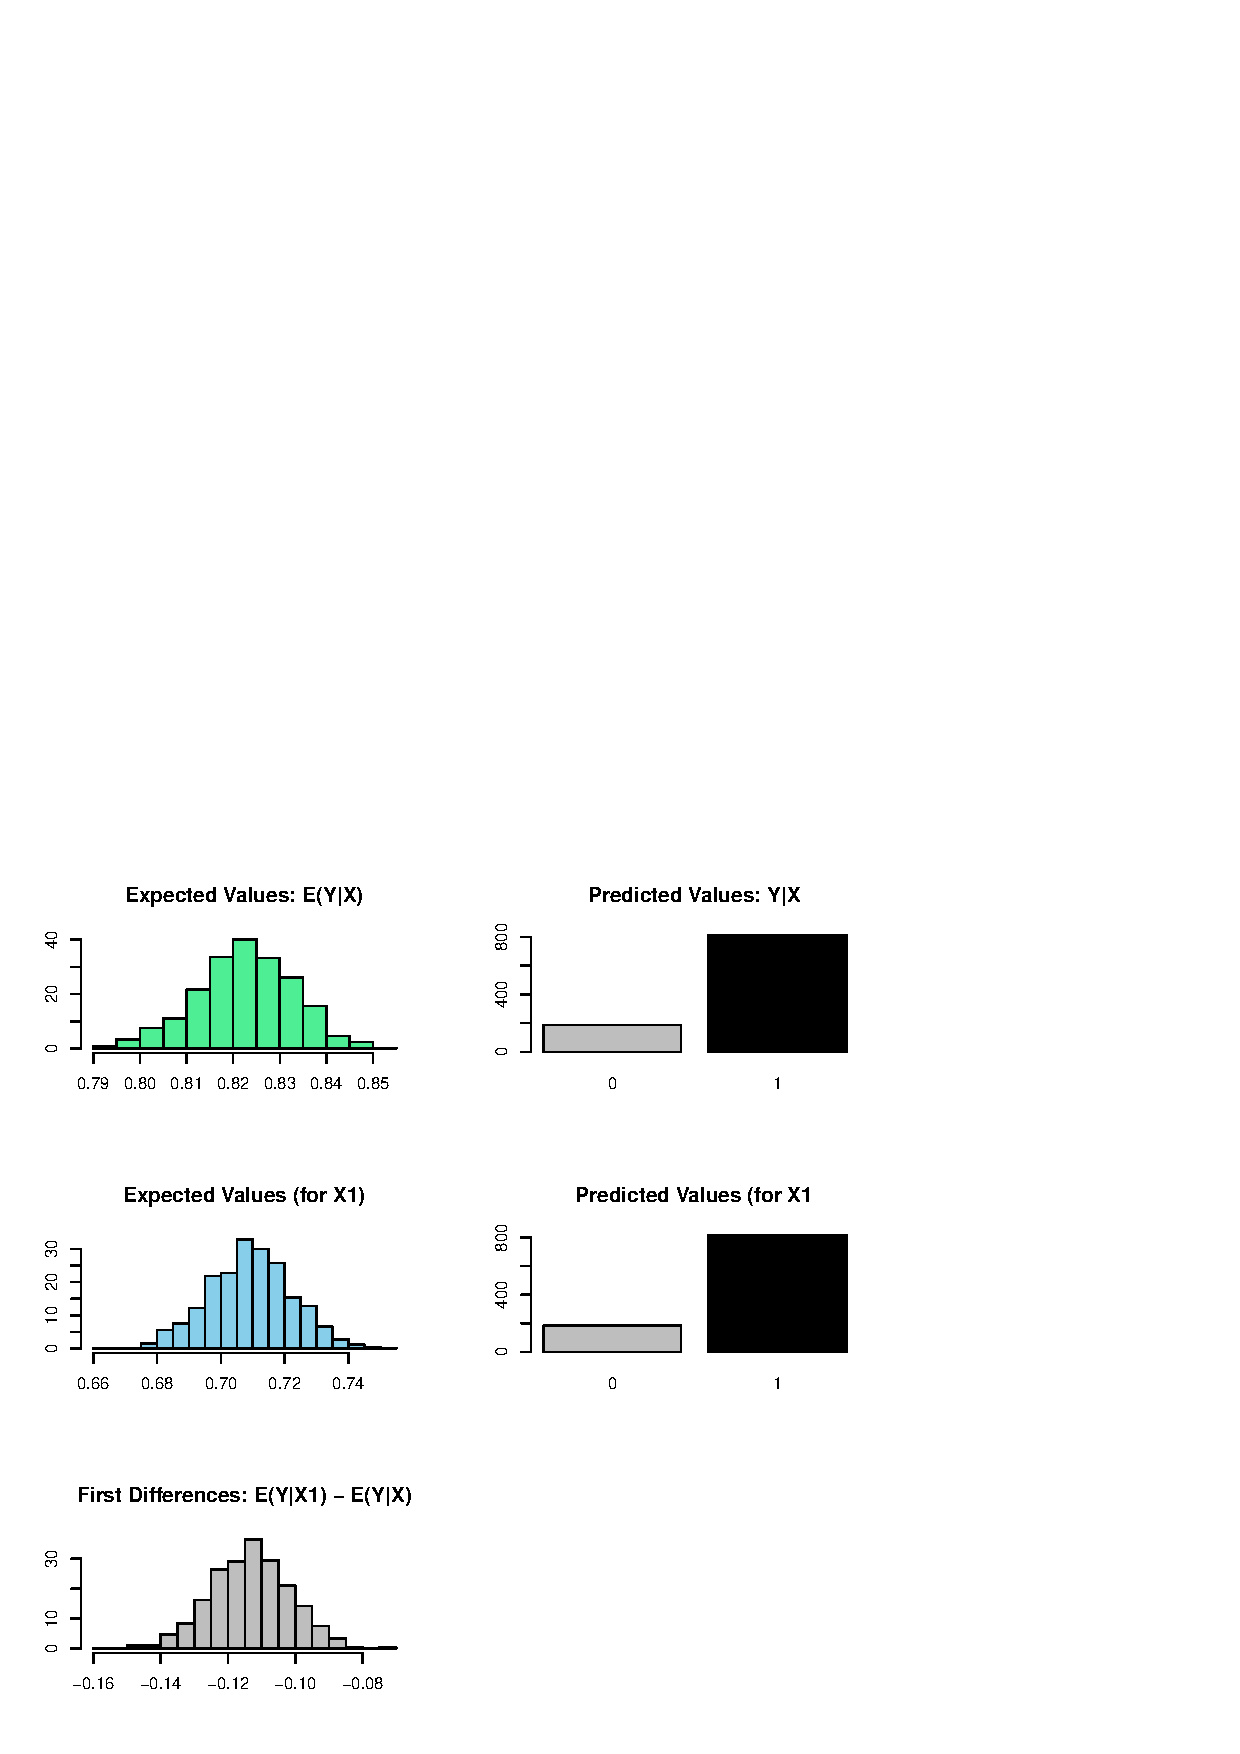
\includegraphics{vigpics/logit-FirstDifferencesPlot}
\end{center} 


\item {Presenting Results: An ROC Plot}  \label{ROC}
  
  One can use an ROC plot to evaluate the fit of alternative model
  specifications.  (Use {\tt demo(roc)} to view this example, or see
  King and Zeng (2002)\nocite{KinZen02}.)  
\begin{Schunk}
\begin{Sinput}
> z.out1 <- zelig(vote ~ race + educate + age, model = "logit", 
+     data = turnout)
> z.out2 <- zelig(vote ~ race + educate, model = "logit", data = turnout)
\end{Sinput}
\end{Schunk}
\begin{center}
\begin{Schunk}
\begin{Sinput}
> rocplot(z.out1$y, z.out2$y, fitted(z.out1), fitted(z.out2))
\end{Sinput}
\end{Schunk}
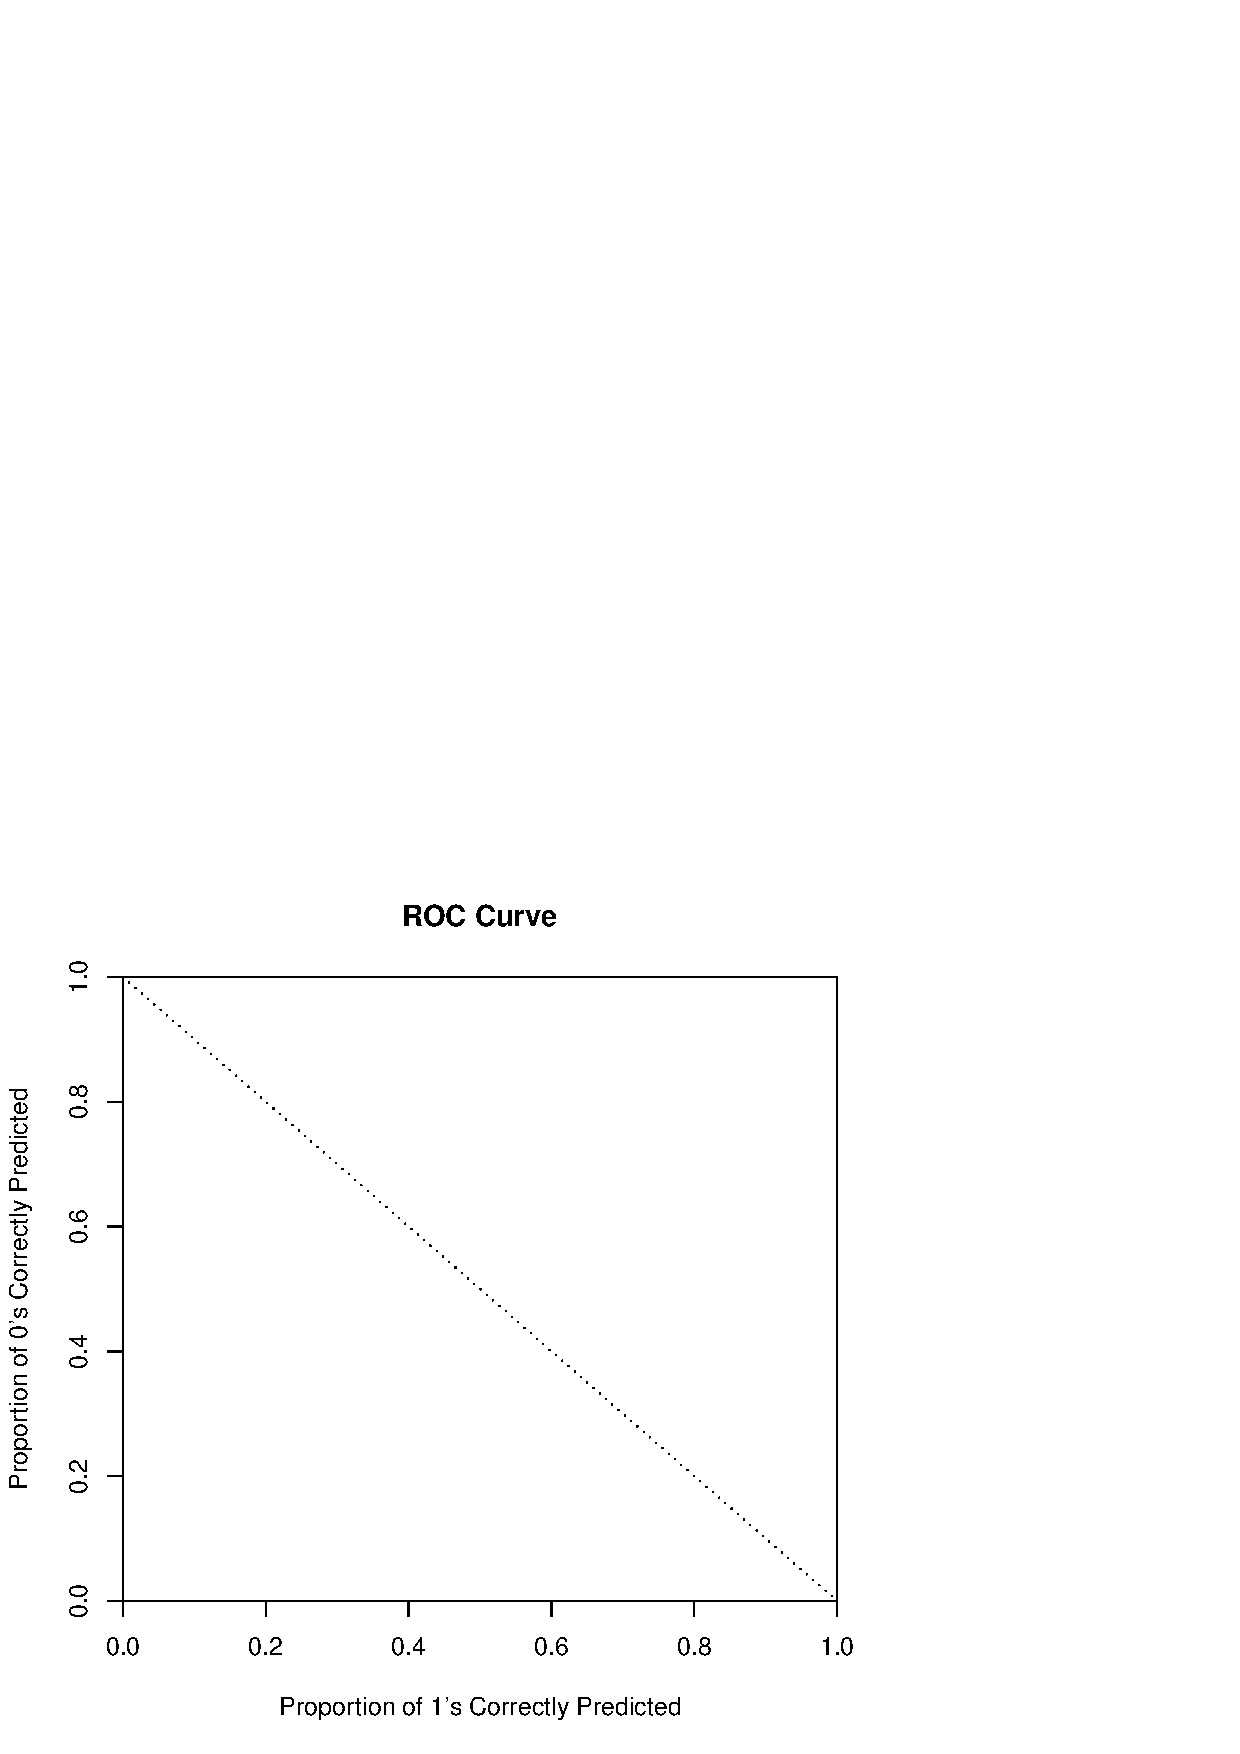
\includegraphics{vigpics/logit-ROCPlot}
\end{center}
\end{enumerate}

\subsubsection{Model}
Let $Y_i$ be the binary dependent variable for observation $i$ which
takes the value of either 0 or 1.
\begin{itemize}

\item The \emph{stochastic component} is given by  
\begin{eqnarray*}
Y_i &\sim& \textrm{Bernoulli}(y_i \mid \pi_i) \\
    &=& \pi_i^{y_i} (1-\pi_i)^{1-y_i}
\end{eqnarray*}
where $\pi_i=\Pr(Y_i=1)$.

\item The \emph{systematic component} is given by: 
\begin{equation*}
\pi_i \; = \; \frac{1}{1 + \exp(-x_i \beta)}.
\end{equation*}
where $x_i$ is the vector of $k$ explanatory variables for observation $i$
and $\beta$ is the vector of coefficients.
\end{itemize}

\subsubsection{Quantities of Interest}
\begin{itemize}
\item The expected values ({\tt qi\$ev}) for the logit model are
  simulations of the predicted probability of a success: $$E(Y) =
  \pi_i= \frac{1}{1 + \exp(-x_i \beta)},$$ given draws of $\beta$ from
  its sampling distribution.

\item The predicted values ({\tt qi\$pr}) are draws from the Binomial
  distribution with mean equal to the simulated expected value $\pi_i$.  

\item The first difference ({\tt qi\$fd}) for the logit model is defined as
\begin{equation*}
\textrm{FD} = \Pr(Y = 1 \mid x_1) - \Pr(Y = 1 \mid x).
\end{equation*}

\item The risk ratio ({\tt qi\$rr}) is defined as
\begin{equation*}
\textrm{RR} = \Pr(Y = 1 \mid x_1) \ / \ \Pr(Y = 1 \mid x).
\end{equation*}

\item In conditional prediction models, the average expected treatment
  effect ({\tt att.ev}) for the treatment group is 
    \begin{equation*} \frac{1}{\sum_{i=1}^n t_i}\sum_{i:t_i=1}^n \left\{ Y_i(t_i=1) -
      E[Y_i(t_i=0)] \right\},
    \end{equation*} 
    where $t_i$ is a binary explanatory variable defining the treatment
    ($t_i=1$) and control ($t_i=0$) groups.  Variation in the
    simulations are due to uncertainty in simulating $E[Y_i(t_i=0)]$,
    the counterfactual expected value of $Y_i$ for observations in the
    treatment group, under the assumption that everything stays the
    same except that the treatment indicator is switched to $t_i=0$.

\item In conditional prediction models, the average predicted treatment
  effect ({\tt att.pr}) for the treatment group is 
    \begin{equation*} \frac{1}{\sum_{i=1}^n t_i}\sum_{i:t_i=1}^n \left\{ Y_i(t_i=1) -
      \widehat{Y_i(t_i=0)}\right\},
    \end{equation*} 
    where $t_i$ is a binary explanatory variable defining the
    treatment ($t_i=1$) and control ($t_i=0$) groups.  Variation in
    the simulations are due to uncertainty in simulating
    $\widehat{Y_i(t_i=0)}$, the counterfactual predicted value of
    $Y_i$ for observations in the treatment group, under the
    assumption that everything stays the same except that the
    treatment indicator is switched to $t_i=0$.
\end{itemize}

\subsubsection{Output Values}

The output of each Zelig command contains useful information which you
may view.  For example, if you run \texttt{z.out <- zelig(y \~\, x,
  model = "logit", data)}, then you may examine the available
information in \texttt{z.out} by using \texttt{names(z.out)},
see the {\tt coefficients} by using {\tt z.out\$coefficients}, and
a default summary of information through \texttt{summary(z.out)}.
Other elements available through the {\tt \$} operator are listed
below.

\begin{itemize}
\item From the {\tt zelig()} output object {\tt z.out}, you may
  extract:
   \begin{itemize}
   \item {\tt coefficients}: parameter estimates for the explanatory
     variables.
   \item {\tt residuals}: the working residuals in the final iteration
     of the IWLS fit.
   \item {\tt fitted.values}: the vector of fitted values for the
     systemic component, $\pi_i$.
   \item {\tt linear.predictors}: the vector of $x_{i}\beta$
   \item {\tt aic}: Akaike's Information Criterion (minus twice the
     maximized log-likelihood plus twice the number of coefficients).
   \item {\tt df.residual}: the residual degrees of freedom.
   \item {\tt df.null}: the residual degrees of freedom for the null
     model.
   \item {\tt data}: the name of the input data frame.  
   \end{itemize}

\item From {\tt summary(z.out)}, you may extract: 
   \begin{itemize}
   \item {\tt coefficients}: the parameter estimates with their
     associated standard errors, $p$-values, and $t$-statistics.
   \item{\tt cov.scaled}: a $k \times k$ matrix of scaled covariances.
   \item{\tt cov.unscaled}: a $k \times k$ matrix of unscaled
     covariances.  
   \end{itemize}

\item From the {\tt sim()} output object {\tt s.out}, you may extract
  quantities of interest arranged as matrices indexed by simulation
  $\times$ {\tt x}-observation (for more than one {\tt x}-observation).
  Available quantities are:

   \begin{itemize}
   \item {\tt qi\$ev}: the simulated expected probabilities for the
     specified values of {\tt x}.
   \item {\tt qi\$pr}: the simulated predicted values for the
     specified values of {\tt x}.
   \item {\tt qi\$fd}: the simulated first difference in the expected
     probabilities for the values specified in {\tt x} and {\tt x1}.
   \item {\tt qi\$rr}: the simulated risk ratio for the expected
     probabilities simulated from {\tt x} and {\tt x1}.
   \item {\tt qi\$att.ev}: the simulated average expected treatment
     effect for the treated from conditional prediction models.  
   \item {\tt qi\$att.pr}: the simulated average predicted treatment
     effect for the treated from conditional prediction models.  
   \end{itemize}
\end{itemize}

\subsection* {How to Cite} 

How to cite this model in Zelig:
\begin{verse}
  Kosuke Imai, Gary King, and Olivia Lau. 2008. "logit: Logistic Regression for Dichotomous Dependent Variables" in Kosuke Imai, Gary King, and Olivia Lau, "Zelig: Everyone's Statistical Software,"http://gking.harvard.edu/zelig
\end{verse}


\CiteZelig

\subsection*{See also}

The logit model is part of the stats package by \citet{VenRip02}.
Advanced users may wish to refer to \texttt{help(glm)} and
\texttt{help(family)}, as well as \cite{McCNel89}. Robust standard
errors are implemented via the sandwich package by \citet{Zeileis04}.
Sample data are from \cite{KinTomWit00}.

\bibliographystyle{asa}
\bibliography{gk,gkpubs}
 



\chapter{Probit Regression for Dichotomous Dependent Variables}

\nobibliography*


\section{{\tt probit}: Probit Regression for Dichotomous Dependent Variables}\label{probit}

Use probit regression to model binary dependent variables
specified as a function of a set of explanatory variables.  For a
Bayesian implementation of this model, see \Sref{probit.bayes}.  

\subsubsection{Syntax}
\begin{verbatim}
> z.out <- zelig(Y ~ X1 + X2, model = "probit", data = mydata)
> x.out <- setx(z.out)
> s.out <- sim(z.out, x = x.out, x1 = NULL)
\end{verbatim}

\subsubsection{Additional Inputs} 

In addition to the standard inputs, {\tt zelig()} takes the following
additional options for probit regression:  
\begin{itemize}
\item {\tt robust}: defaults to {\tt FALSE}.  If {\tt TRUE} is
selected, {\tt zelig()} computes robust standard errors via the {\tt
sandwich} package (see \cite{Zeileis04}).  The default type of robust
standard error is heteroskedastic and autocorrelation consistent (HAC),
and assumes that observations are ordered by time index.

In addition, {\tt robust} may be a list with the following options:  
\begin{itemize}
\item {\tt method}:  Choose from 
\begin{itemize}
\item {\tt "vcovHAC"}: (default if {\tt robust = TRUE}) HAC standard
errors. 
\item {\tt "kernHAC"}: HAC standard errors using the
weights given in \cite{Andrews91}. 
\item {\tt "weave"}: HAC standard errors using the
weights given in \cite{LumHea99}.  
\end{itemize}  
\item {\tt order.by}: defaults to {\tt NULL} (the observations are
chronologically ordered as in the original data).  Optionally, you may
specify a vector of weights (either as {\tt order.by = z}, where {\tt
z} exists outside the data frame; or as {\tt order.by = \~{}z}, where
{\tt z} is a variable in the data frame).  The observations are
chronologically ordered by the size of {\tt z}.
\item {\tt \dots}:  additional options passed to the functions 
specified in {\tt method}.   See the {\tt sandwich} library and
\cite{Zeileis04} for more options.   
\end{itemize}
\end{itemize}

\subsubsection{Examples}
Attach the sample turnout dataset:
\begin{Schunk}
\begin{Sinput}
> data(turnout)
\end{Sinput}
\end{Schunk}
Estimate parameter values for the probit regression:
\begin{Schunk}
\begin{Sinput}
> z.out <- zelig(vote ~ race + educate, model = "probit", data = turnout)
\end{Sinput}
\end{Schunk}
\begin{Schunk}
\begin{Sinput}
> summary(z.out)
\end{Sinput}
\end{Schunk}
Set values for the explanatory variables to their default values.
\begin{Schunk}
\begin{Sinput}
> x.out <- setx(z.out)
\end{Sinput}
\end{Schunk}
Simulate quantities of interest from the posterior distribution.
\begin{Schunk}
\begin{Sinput}
> s.out <- sim(z.out, x = x.out)
\end{Sinput}
\end{Schunk}
\begin{Schunk}
\begin{Sinput}
> summary(s.out)
\end{Sinput}
\end{Schunk}

\subsubsection{Model}
Let $Y_i$ be the observed binary dependent variable for observation
$i$ which takes the value of either 0 or 1.
\begin{itemize}
\item The \emph{stochastic component} is given by  
\begin{equation*}
Y_i \; \sim \; \textrm{Bernoulli}(\pi_i), 
\end{equation*}
where $\pi_i=\Pr(Y_i=1)$.

\item The \emph{systematic component} is 
\begin{equation*}
  \pi_i \; = \; \Phi (x_i \beta)
\end{equation*}
where $\Phi(\mu)$ is the cumulative distribution function of the
Normal distribution with mean 0 and unit variance.
\end{itemize}

\subsubsection{Quantities of Interest}

\begin{itemize}

\item The expected value ({\tt qi\$ev}) is a simulation of predicted
  probability of success $$E(Y) = \pi_i = \Phi(x_i
  \beta),$$ given a draw of $\beta$ from its sampling distribution.  

\item The predicted value ({\tt qi\$pr}) is a draw from a Bernoulli
  distribution with mean $\pi_i$.  
  
\item The first difference ({\tt qi\$fd}) in expected values is
  defined as
\begin{equation*}
\textrm{FD} = \Pr(Y = 1 \mid x_1) - \Pr(Y = 1 \mid x).
\end{equation*}

\item The risk ratio ({\tt qi\$rr}) is defined as
\begin{equation*}
\textrm{RR} = \Pr(Y = 1 \mid x_1) / \Pr(Y = 1 \mid x).
\end{equation*}

\item In conditional prediction models, the average expected treatment
  effect ({\tt att.ev}) for the treatment group is 
    \begin{equation*} \frac{1}{\sum_{i=1}^n t_i}\sum_{i:t_i=1}^n \left\{ Y_i(t_i=1) -
      E[Y_i(t_i=0)] \right\},
    \end{equation*} 
    where $t_i$ is a binary explanatory variable defining the treatment
    ($t_i=1$) and control ($t_i=0$) groups.  Variation in the
    simulations are due to uncertainty in simulating $E[Y_i(t_i=0)]$,
    the counterfactual expected value of $Y_i$ for observations in the
    treatment group, under the assumption that everything stays the
    same except that the treatment indicator is switched to $t_i=0$.

\item In conditional prediction models, the average predicted treatment
  effect ({\tt att.pr}) for the treatment group is 
    \begin{equation*} \frac{1}{\sum_{i=1}^n t_i}\sum_{i:t_i=1}^n \left\{ Y_i(t_i=1) -
      \widehat{Y_i(t_i=0)} \right\},
    \end{equation*} 
    where $t_i$ is a binary explanatory variable defining the
    treatment ($t_i=1$) and control ($t_i=0$) groups.  Variation in
    the simulations are due to uncertainty in simulating
    $\widehat{Y_i(t_i=0)}$, the counterfactual predicted value of
    $Y_i$ for observations in the treatment group, under the
    assumption that everything stays the same except that the
    treatment indicator is switched to $t_i=0$.
\end{itemize}

\subsubsection{Output Values}

The output of each Zelig command contains useful information which you
may view.  For example, if you run \texttt{z.out <- zelig(y \~\,
  x, model = "probit", data)}, then you may examine the available
information in \texttt{z.out} by using \texttt{names(z.out)},
see the {\tt coefficients} by using {\tt z.out\$coefficients}, and
a default summary of information through \texttt{summary(z.out)}.
Other elements available through the {\tt \$} operator are listed
below.

\begin{itemize}
\item From the {\tt zelig()} output object {\tt z.out}, you may extract:
   \begin{itemize}
   \item {\tt coefficients}: parameter estimates for the explanatory
     variables.
   \item {\tt residuals}: the working residuals in the final iteration
     of the IWLS fit.
   \item {\tt fitted.values}: a vector of the in-sample fitted values.
   \item {\tt linear.predictors}: a vector of $x_{i}\beta$.  
   \item {\tt aic}: Akaike's Information Criterion (minus twice the
     maximized log-likelihood plus twice the number of coefficients).
   \item {\tt df.residual}: the residual degrees of freedom.
   \item {\tt df.null}: the residual degrees of freedom for the null
     model.
   \item {\tt data}: the name of the input data frame.  
   \end{itemize}

\item From {\tt summary(z.out)}, you may extract: 
   \begin{itemize}
   \item {\tt coefficients}: the parameter estimates with their
     associated standard errors, $p$-values, and $t$-statistics.
   \item{\tt cov.scaled}: a $k \times k$ matrix of scaled covariances.
   \item{\tt cov.unscaled}: a $k \times k$ matrix of unscaled
     covariances.  
   \end{itemize}

\item From the {\tt sim()} output object {\tt s.out}, you may extract
  quantities of interest arranged as matrices indexed by simulation
  $\times$ {\tt x}-observation (for more than one {\tt x}-observation).
  Available quantities are:

   \begin{itemize}
   \item {\tt qi\$ev}: the simulated expected values, or predicted
     probabilities, for the specified values of {\tt x}.
   \item {\tt qi\$pr}: the simulated predicted values drawn from the
     distributions defined by the predicted probabilities.  
   \item {\tt qi\$fd}: the simulated first differences in the predicted
     probabilities for the values specified in {\tt x} and {\tt x1}.
   \item {\tt qi\$rr}: the simulated risk ratio for the predicted
     probabilities simulated from {\tt x} and {\tt x1}.
   \item {\tt qi\$att.ev}: the simulated average expected treatment
     effect for the treated from conditional prediction models.  
   \item {\tt qi\$att.pr}: the simulated average predicted treatment
     effect for the treated from conditional prediction models.  
   \end{itemize}
\end{itemize}


\subsection* {How to Cite} 

How to cite this model in Zelig:

\begin{verse}
  Kosuke Imai, Gary King, and Olivia Lau. 2007. "probit: Probit Regression for Dichotomous Dependent Variables" in Kosuke Imai, Gary King, and Olivia Lau, "Zelig: Everyone's Statistical Software,"http://gking.harvard.edu/zelig
\end{verse}

\CiteZelig


\subsection* {See also}
The probit model is part of the stats package by \citet{VenRip02}.
Advanced users may wish to refer to \texttt{help(glm)} and
\texttt{help(family)}, as well as \cite{McCNel89}. Robust standard
errors are implemented via the sandwich package by \citet{Zeileis04}.
Sample data are from \cite{KinTomWit00}.

\bibliographystyle{asa}
\bibliography{gk,gkpubs}
 



% end body
\end{document}
\include{commandsRd/setx}
\include{commandsRd/sim}
\section{{\tt summary}: Summarizing Zelig Output}
\label{ss:summary}

\subsubsection{Description}

Summarize R objects using using the generic function {\tt summary()}.
R automatically recognizes the type of object (lists, data frames,
variables, etc.) and selects the appropriate {\tt summary()} function.

\subsubsection{Syntax}

\begin{verbatim}
> summary(z.out, subset = NULL, ...)
> summary(s.out, subset = NULL, CI = 95, 
          stats = c("mean", "sd", "min", "max"), ...)
\end{verbatim}
To set the desired number of digits in the summary output, use {\tt
  options(digits = x)}, where {\tt x} is the desired number of digits,
prior to using the {\tt summary()} command.

\subsubsection{Arguments for multiply-imputed {\tt zelig()} output}
For {\tt zelig()} output created with $m$ multiply-imputed data sets,
the {\tt z.out} object contains one set of output for each imputed
data set.  Options for multiply-imputed {\tt zelig()} output include:
   \begin{itemize}
   \item {\tt subset}: specifies which of the $m$ sets of output to
     summarize.  Possible arguments include:
       \begin{itemize}
       \item {\tt NULL}: (default) which produces one summary by
         averaging the coefficients and standard errors from all the
         imputed data sets using the Rubin rules (\hlink{King,
           Honaker, Joseph, Scheve
           (2000)}{http://gking.harvard.edu/files/abs/evil-abs.shtml},
         p. 53).
       \item a numeric vector: consisting of any set of numbers in
         $[1,m]$.  For example, you may use {\tt summary(z.out,
           subset = 2:4)} to view the output from the second, third,
         and fourth imputed data sets only.  
       \end{itemize}
     \item{\dots}: additional options passed to {\tt print()}.  
    \end{itemize}

\subsubsection{Arguments for subsetted {\tt zelig()} output}
If you selected the {\tt by} option, {\tt zelig()} creates an {\tt
  z.out} object with one set of regression output for each of the
unique values in the {\tt by} variable.  Options for subsetted
  analyses are:  
\begin{itemize}
\item {\tt subset}: specifies which regression output to summarize.
  You cannot summarize multiple analyses generated using the {\tt
    "by"} option in one summary, as each of the levels in the {\tt by}
  variable may have a different number of associated observations.  (A
  weighted summary would also be inappropriate, as the weighted
  coefficients would be identical to the coefficients generated
  without subsetting.)
\begin{itemize}
\item numeric vector: specifying which sets of regression output to
  summarize.  By default, {\tt summary()} for subsetted output
  sequentially summarizes the regression output for each unique value
  in the {\tt by} variable.  You may choose to summarize just the
  fifteenth unique value by typing:  {\tt summary(z.out, subset =
    15)}.  
\end{itemize}
\item {\tt \dots}: Additional arguments passed to {\tt print()}.
\end{itemize}
   
\subsubsection{Arguments for {\tt sim()} output}
Summaries of {\tt sim()} output includes these additional options:
   \begin{itemize}
     \item {\tt subset}:  Only valid for {\tt sim()} output created
       using more than one observation in {\tt x}.  You may select to
       summarize the quantities of interest created by each
       observation in {\tt x} using one of the following options: 
       \begin{itemize}
       \item {\tt NULL}: (default) produces one summary per quantity
         of interest by combining the simulations from each
         observation into a single set and then summarizing.
         \item {\tt all}:  summarizes the quantity of interest
           produced by each observation separately.  
         \item a numeric vector: specifying the observations to summarize 
       \end{itemize}
     \item {\tt CI}: A value between 0 and 100, for the percentage
       confidence interval.  The default value is 95, for a 95 percent
       confidence interval.  
     \item {\tt stats}: A vector specifying the statistics to
       calculate for each quantity of interest.  The default values
       are {\tt c("mean", "sd", "min", "max")}.  
   \end{itemize}
Using {\tt summary()} on {\tt sim()} output from multiple analyses
will automatically weight the quantities of interest according to the
proportion of observations in each strata.  

\subsubsection{Output Values}
\begin{itemize}
\item For {\tt zelig()} output objects, {\tt summary()} returns a
  formatted summary of the regression output, including the usual
  table of coefficients, standard errors, and $t$-values.  Additional
  output depends on the statistical model, the names of which may
  be viewed using the {\tt names(summary(z.out))} command.
\item For {\tt sim()} output objects, {\tt summary()} returns summary
  statistics for each quantity of interest, including a default 95\%
  confidence interval.  Use {\tt names(summary(s.out))} to see the
  available output.  Note that {\tt qi.stats} contains a useful matrix
  of summary statistics for each of the quantities of interest.  For
  example, {\tt summary(s.out)\$qi.stats\$ev}, extracts the summary
  matrix of expected values.
\end{itemize}

\subsubsection{See Also}

Advanced users may wish to refer to {\tt help.zelig("print")},
as well as {\tt help(summary)}, {\tt help(summary.lm)}, {\tt
  help(summary.glm)}, and {\tt help(anova)} in the base package.

\subsubsection{Contributors}

Kosuke Imai, Gary King, and Olivia Lau added summary methods for
certain {\tt zelig()} models, and for {\tt sim()} output.


%%% Local Variables: 
%%% mode: latex
%%% TeX-master: t
%%% End: 


\include{commandsRd/plot.zelig}
\section{{\tt print}: Printing Quantities of Interest}
\label{ss:print}

\subsubsection{Description}
The {\tt print} command formats summary output and allows users to
specify the number of decimal places as an optional argument.  

\subsubsection{Syntax}
\begin{verbatim}
> print(x, digits = 3, print.x = FALSE)
\end{verbatim}

\subsubsection{Arguments}

\begin{itemize}
\item {\tt x}: the object to be printed may be {\tt z.out} output
  from {\tt zelig()}, {\tt x.out} output from {\tt setx()}, {\tt s.out}
  output from {\tt sim()}, or other R data structures.
\item {\tt digits}: the minimum number of significant digits to return
  for all elements of $x < 0$.  By default, {\tt print()} avoids
  scientific notation, but setting the number of digits to 1 will
  frequently force output in scientific notation.  The number of {\tt
    digits} is not the number of significant digits for all output
  values, but the minimum number of significant digits for the
  smallest value in {\tt x} between -1 and 1; this governs the number
  of significant digits in the rest of the values with decimal output.
\item {\tt print.x}: a logical value for {\tt sim()} output, which
  specifies whether to print a summary ({\tt print.x = FALSE}, the
  default) of the {\tt x} and {\tt x1} \emph{inputs} to {\tt sim()},
  or the complete set of inputs (optionally, {\tt print.x = TRUE}).
\end{itemize}

\subsubsection{Examples}
\begin{verbatim}
> print(summary(z.out), digits = 2)
> print(summary(s.out), digits = 3, print.x = TRUE)
\end{verbatim}

\subsubsection{See Also}

Advanced users may wish to refer to {\tt help(print)}.

\subsubsection{Contributors}

Kosuke Imai, Gary King, and Olivia Lau added print methods for {\tt
  sim()} output, and {\tt summary()} output for Zelig objects.   

%%% Local Variables: 
%%% mode: latex
%%% TeX-master: t
%%% End: 

\include{commandsRd/repl}

\chapter{Supplementary Commands}

\section{{\tt matchit}: Create matched data}\label{matchit}

\subsubsection{Description}

\hlink{MatchIt}{http://gking.harvard.edu/matchit/} implements the
suggestions of \cite{HoImaKin05b} for improving parametric statistical
models by preprocessing data with semi-parametric matching methods. It
uses a sophisticated array of matching methods to select well-matched
treated and control units from the original data set, thus reducing
the dependence of causal inferences on functional form and other
parametric assumptions.  After pre-processing, MatchIt output can be
used just like any other dataset in Zelig to estimate causal effects.
In this way, MatchIt improves rather than replaces existing parametric
models, reducing sensitivity to modeling assumptions.  The matching
methods available in
\hlink{MatchIt}{http://gking.harvard.edu/matchit/} include exact
matching on all covariates, nearest neighbor matching,
subclassification, optimal matching, genetic matching, and full
matching.  An outline of all options are provided below; see the full
documentation (available at
\hlink{\url{http://gking.harvard.edu/matchit/}}{http://gking.harvard.edu/matchit/})
for more details.

\subsubsection{Syntax}
\begin{verbatim}
> m.out <- matchit(formula, data, method = "nearest", verbose = FALSE, ...)
\end{verbatim}

\subsubsection{Arguments}

\paragraph{Arguments for All Matching Methods}

\begin{itemize}

\item \texttt{formula}: formula used to calculate the distance measure
  for matching.  It takes the usual syntax of R formulas, {\tt treat
    \~\ x1 + x2}, where {\tt treat} is a binary treatment indicator,
  and {\tt x1} and {\tt x2} are the pre-treatment covariates. Both the
  treatment indicator and pre-treatment covariates must be contained
  in the same data frame, which is specified as {\tt data} (see
  below).  All of the usual R syntax for formulas work here. For
  example, {\tt x1:x2} represents the first order interaction term
  between {\tt x1} and {\tt x2}, and {\tt I(x1 \^\ 2)} represents the
  square term of {\tt x1}. See {\tt help(formula)} for details.
  
\item \texttt{data}: the data frame containing the variables called in
  {\tt formula}.  
  
\item \texttt{method}: the matching method (default =
  \texttt{"nearest"}, nearest neighbor matching).  Currently,
  \texttt{"exact"} (exact matching), \texttt{"full"} (full matching),
  \texttt{"nearest"} (nearest neighbor matching), \texttt{"optimal"}
  (optimal matching), \texttt{"subclass"} (subclassification), and
  \texttt{"genetic"} (genetic matching) are available. Note that
  within each of these matching methods, \MatchIt\ offers a variety of
  options. See below for more details.
  
\item \texttt{verbose}: a logical value indicating whether to print
  the status of the matching algorithm (default = \texttt{FALSE}).
\end{itemize}


\paragraph{Additional Arguments for Specification of
  Distance Measures}
\label{subsubsec:inputs-all}

The following arguments specify distance measures that are used for
matching methods. These arguments apply to all matching methods {\it
  except exact matching}.

\begin{itemize}
  
\item \texttt{distance}: the method used to estimate the distance
  measure (default = {\tt "logit"}, logistic regression) or a
  numerical vector of user's own distance measure.  Before using any
  of these techniques, it is best to understand the theoretical
  groundings of these techniques and to evaluate the results.  Most of
  these methods (such as logistic or probit regression) estimate the
  propensity score, defined as the probability of receiving treatment,
  conditional on the covariates.  Available methods include:
  \begin{itemize}
  \item {\tt "mahalanobis"}: the Mahalanobis distance measure.
  \item binomial generalized linear models with one of the following
    link functions:
    \begin{itemize}
    \item \texttt{"logit"}: logistic link 
    \item {\tt "linear.logit"}: logistic link with linear propensity
      score)\footnote{The linear propensity scores are obtained by
        transforming back onto a linear scale.}
    \item \texttt{"probit"}: probit link
    \item {\tt "linear.probit"}: probit link with linear propensity
      score
    \item {\tt "cloglog"}: complementary log-log link
    \item {\tt "linear.cloglog"}: complementary log-log link with linear
      propensity score
    \item {\tt "log"}: log link
    \item {\tt "linear.log"}: log link with linear propensity score
    \item {\tt "cauchit"} Cauchy CDF link
    \item {\tt "linear.cauchit"} Cauchy CDF link with linear propensity
      score
    \end{itemize}
  \item Choose one of the following generalized additive models (see
    {\tt help(gam)} for more options).
    \begin{itemize}
    \item \texttt{"GAMlogit"}: logistic link
    \item {\tt "GAMlinear.logit"}: logistic link with linear propensity
      score
    \item \texttt{"GAMprobit"}: probit link
    \item {\tt "GAMlinear.probit"}: probit link with linear propensity
      score
    \item {\tt "GAMcloglog"}: complementary log-log link 
    \item {\tt "GAMlinear.cloglog"}: complementary log-log link with
      linear propensity score
    \item {\tt "GAMlog"}: log link
    \item {\tt "GAMlinear.log"}: log link with linear propensity score,
    \item {\tt "GAMcauchit"}: Cauchy CDF link
    \item {\tt "GAMlinear.cauchit"}: Cauchy CDF link with linear
      propensity score
\end{itemize} 
\item \texttt{"nnet"}: neural network model.  See {\tt help(nnet)} for
  more options.
\item \texttt{"rpart"}: classification trees.  See {\tt help(rpart)}
  for more options.
  \end{itemize}
  
\item \texttt{distance.options}: optional arguments for estimating the
  distance measure. The input to this argument should be a list.  For
  example, if the distance measure is estimated with a logistic
  regression, users can increase the maximum IWLS iterations by
  \texttt{distance.options = list(maxit = 5000)}.  Find additional
  options for general linear models using {\tt help(glm)} or {\tt
    help(family)}, for general additive models using {\tt help(gam)},
  for neutral network models {\tt help(nnet)}, and for classification
  trees {\tt help(rpart)}.
  
\item \texttt{discard}: specifies whether to discard units that fall
  outside some measure of support of the distance measure (default =
  \texttt{"none"}, discard no units).  Discarding units may change the
  quantity of interest being estimated. Enter a logical vector
  indicating which unit should be discarded or choose from the
  following options:
  \begin{itemize}
  \item \texttt{"none"}: no units will be discarded before matching.
    Use this option when the units to be matched are substantially
    similar, such as in the case of matching treatment and control
    units from a field experiment that was close to (but not fully)
    randomized (e.g., \citealt{Imai05}), when caliper matching will
    restrict the donor pool, or when you do not wish to change the
    quantity of interest and the parametric methods to be used
    post-matching can be trusted to extrapolate.
  \item \texttt{"hull.both"}: all units that are not within the convex
    hull will be discarded.  We recommend that this option be used
    with observational data sets.
  \item \texttt{"both"}: all units (treated and control) that are
    outside the support of the distance measure will be discarded.
  \item \texttt{"hull.control"}: only control units that are not
    within the convex hull of the treated units will be discarded.  
  \item \texttt{"control"}: only control units outside the support of
    the distance measure of the treated units will be discarded.  Use
    this option when the average treatment effect on the treated is of
    most interest and when you are unwilling to discard
    non-overlapping treatment units (which would change the quantity
    of interest).
  \item \texttt{"hull.treat"}: only treated units that are not within
    the convex hull of the control units will be discarded. 
  \item \texttt{"treat"}: only treated units outside the support of
    the distance measure of the control units will be discarded.  Use
    this option when the average treatment effect on the control units
    is of most interest and when unwilling to discard control units.
  \end{itemize}
  
\item \texttt{reestimate}: If {\tt FALSE} (default), the model for the
  distance measure will not be re-estimated after units are discarded.
  The input must be a logical value.  Re-estimation may be desirable
  for efficiency reasons, especially if many units were discarded and
  so the post-discard samples are quite different from the original
  samples.
  
\end{itemize}

\paragraph{Additional Arguments for Subclassification}
\label{subsubsec:inputs-subclass}

\begin{itemize}
\item \texttt{sub.by}: criteria for subclassification.  Choose from:
  \texttt{"treat"} (default), the number of treatment units;
  \texttt{"control"}, the number of control units; or \texttt{"all"},
  the total number of units.
\item \texttt{subclass}: either a scalar specifying the number of
  subclasses, or a vector of probabilities bounded between 0 and 1,
  which create quantiles of the distance measure using the units in
  the group specified by \texttt{sub.by} (default = \texttt{subclass =
    6}).
\end{itemize}

\paragraph{Additional Arguments for Nearest Neighbor Matching}
\label{subsubsec:inputs-nearest}

\begin{itemize}
\item \texttt{m.order}: the order in which to match treatment units
  with control units.
  \begin{itemize}
  \item {\tt "largest"} (default): matches from the largest value of
    the distance measure to the smallest.
  \item {\tt "smallest"}: matches from the smallest value of the
    distance measure to the largest.
  \item {\tt "random"}: matches in random order.
  \end{itemize}
\item \texttt{replace}: logical value indicating whether each control
  unit can be matched to more than one treated unit (default = {\tt
    replace = FALSE}, each control unit is used at most once -- i.e.,
  sampling without replacement). For matching with replacement, use
  \texttt{replace = TRUE}.
\item \texttt{ratio}: the number of control units to match to each
  treated unit (default = {\tt 1}).  If matching is done without
  replacement and there are fewer control units than {\tt ratio} times
  the number of eligible treated units (i.e., there are not enough
  control units for the specified method), then the higher ratios will
  have \texttt{NA} in place of the matching unit number in
  \texttt{match.matrix}.
\item \texttt{exact}: variables on which to perform exact matching
  within the nearest neighbor matching (default = {\tt NULL}, no exact
  matching).  If \texttt{exact} is specified, only matches that
  exactly match on the covariates in \texttt{exact} will be allowed.
  Within the matches that match on the variables in \texttt{exact},
  the match with the closest distance measure will be chosen.
  \texttt{exact} should be entered as a vector of variable names
  (e.g., \texttt{exact = c("X1", "X2")}).
\item \texttt{caliper}: the number of standard deviations of the
  distance measure within which to draw control units (default = {\tt
    0}, no caliper matching).  If a caliper is specified, a control
  unit within the caliper for a treated unit is randomly selected as
  the match for that treated unit.  If \texttt{caliper != 0}, there
  are two additional options:
  \begin{itemize} 
  \item \texttt{calclosest}: whether to take the nearest available
    match if no matches are available within the \texttt{caliper}
    (default = {\tt FALSE}).
  \item \texttt{mahvars}: variables on which to perform
    Mahalanobis-metric matching within each caliper (default = {\tt
      NULL}).  Variables should be entered as a vector of variable
    names (e.g., \texttt{mahvars = c("X1", "X2")}).  If
    \texttt{mahvars} is specified without \texttt{caliper}, the
    caliper is set to 0.25.
  \end{itemize}
\item \texttt{subclass} and \texttt{sub.by}: See the options for
  subclassification for more details on these options.  If a
  \texttt{subclass} is specified within \texttt{method = "nearest"},
  the matched units will be placed into subclasses after the nearest
  neighbor matching is completed.
\end{itemize}

\paragraph{Additional Arguments for Optimal Matching}
\label{subsubsec:inputs-optimal}

\begin{itemize}
\item {\tt ratio}: the number of control units to be matched to each
  treatment unit (default = {\tt 1}).
\item {\tt ...}: additional inputs that can be passed to the {\tt
    fullmatch()} function in the {\tt optmatch} package. See {\tt
    help(fullmatch)} or
  \hlink{http://www.stat.lsa.umich.edu/\~{}bbh/optmatch.html}{http://www.stat.lsa.umich.edu/~bbh/optmatch.html}
  for details.
\end{itemize}

\paragraph{Additional Arguments for Full Matching}
\label{subsubsec:inputs-full}

\begin{itemize}
\item {\tt ...}: additional inputs that can be passed to the {\tt
    fullmatch()} function in the {\tt optmatch} package. See {\tt
    help(fullmatch)} or
  \hlink{http://www.stat.lsa.umich.edu/\~{}bbh/optmatch.html}{http://www.stat.lsa.umich.edu/~bbh/optmatch.html} for details.
\end{itemize}

\paragraph{Additional Arguments for Genetic Matching}
\label{subsubsec:inputs-genetic}

The available options are listed below.
\begin{itemize}
\item {\tt ratio}: the number of control units to be matched to each
  treatment unit (default = {\tt 1}).
\item {\tt ...}: additional minor inputs that can be passed to the
  {\tt GenMatch()} function in the {\tt Matching} package. See {\tt
    help(GenMatch)} or
  \hlink{http://sekhon.polisci.berkeley.edu/library/Matching/html/GenMatch.html}{http://sekhon.polisci.berkeley.edu/library/Matching/html/GenMatch.html}
  for details.
\end{itemize}

\subsubsection{Output Values}
\label{sec:outputs}

Regardless of the type of matching performed, the \texttt{matchit}
output object contains the following elements:\footnote{When
  inapplicable or unnecessary, these elements may equal {\tt NULL}.
  For example, when exact matching, {\tt match.matrix = NULL}.}

\begin{itemize}
\item \texttt{call}: the original {\tt matchit()} call.
  
\item \texttt{formula}: the formula used to specify the model for
  estimating the distance measure.
  
\item \texttt{model}: the output of the model used to estimate
  the distance measure.  \texttt{summary(m.out\$model)} will give the
  summary of the model where \texttt{m.out} is the output object from
  \texttt{matchit()}.
  
\item \texttt{match.matrix}: an $n_1 \times$ \texttt{ratio} matrix
  where:
  \begin{itemize}
  \item the row names represent the names of the treatment units
    (which match the row names of the data frame specified in
    \texttt{data}).
  \item each column stores the name(s) of the control unit(s) matched
    to the treatment unit of that row. For example, when the
    \texttt{ratio} input for nearest neighbor or optimal matching is
    specified as 3, the three columns of \texttt{match.matrix}
    represent the three control units matched to one treatment unit).
  \item \texttt{NA} indicates that the treatment unit was not matched.
  \end{itemize}
  
\item \texttt{discarded}: a vector of length $n$ that displays whether
  the units were ineligible for matching due to common support
  restrictions.  It equals \texttt{TRUE} if unit $i$ was discarded,
  and it is set to \texttt{FALSE} otherwise.
  
\item \texttt{distance}: a vector of length $n$ with the estimated
  distance measure for each unit.
  
\item \texttt{weights}: a vector of length $n$ with the weights
  assigned to each unit in the matching process.  Unmatched units have
  weights equal to $0$. Matched treated units have weight $1$.  Each
  matched control unit has weight proportional to the number of
  treatment units to which it was matched, and the sum of the control
  weights is equal to the number of uniquely matched control units.
 
\item \texttt{subclass}: the subclass index in an ordinal scale from 1
  to the total number of subclasses as specified in \texttt{subclass}
  (or the total number of subclasses from full or exact matching).
  Unmatched units have \texttt{NA}.
  
\item \texttt{q.cut}: the subclass cut-points that classify the
  distance measure.
  
\item \texttt{treat}: the treatment indicator from \texttt{data} (the
  left-hand side of \texttt{formula}).
 
\item \texttt{X}: the covariates used for estimating the distance
  measure (the right-hand side of \texttt{formula}).  When applicable,
  \texttt{X} is augmented by covariates contained in \texttt{mahvars}
  and \texttt{exact}.
\end{itemize}

\subsubsection{Contributors}

If you use \MatchIt, please cite
\begin{verse}
\bibentry{HoImaKin07}
and 
\bibentry{HoImaKin05b}
\end{verse}

The {\tt convex.hull} discard option is implemented via the {\tt
  WhatIf} package \citep{StoKinZen06,KinZen06a,KinZen06b}.
Generalized linear distance measures are implemented via the {\tt
  stats} package \citep{VenRip02}.  Generalized additive distance
measures are implemented via the {\tt mcgv} package \citep{HasTib90}.
The neural network distance measure is implemented via the {\tt nnet}
package \citep{Ripley96}.  The classification trees distance measure
is implemented via the {\tt rpart} package \citep{BreFriOls84}.  Full
and optimal matching are implemented via the {\tt optmatch} package
\citep{Hansen04}.  Genetic matching is implemented via the {\tt
  Matching} package \citep{DiaSek05}.

%%% Local Variables: 
%%% mode: latex
%%% TeX-master: "matchit"
%%% End: 

% author: Matt Owen
% documentation for using the 'mi' class
\documentclass[a4paper,11pt]{article}

% Packages
\usepackage{listings}
\lstset{language=R}


\begin{document}


\section*{Fitting Multiple Statistical Models Simultaneously}

It is often important, especially when computing data based on counterfactuals, to have a side-by-side comparison of the different fitted models and their \emph{quantities of interest}.  Typically, the statistician interested in comparing multiple models would:
\begin{itemize}
	\item{Prepare Several Different Datasets, by:}
	\begin{itemize}
		\item{Splitting a Dataset into Several Categorized by Some Particular Quality}
		\item{Preparing Counterfactual Data Based on a Pre-existing Dataset}
		\item{Collecting Several Different Data-sets Analyzing Similar Data}
	\end{itemize}
	\item{Compute a Fitted Model for Each Dataset}
	\item{Simulate Quantities of Interest for Each Fitted Model}
	\item{Organize the Results in a Logical Fashion}
\end{itemize}

This process can be quite arduous, and the programming syntax associated with these sorts of processes is often unintuitive and cumbersome.  Resulting from the necessity to simplify this process, the Zelig software package offers an intuitive and simple syntax to produce these results.

\section{The \emph{mi} class: An Easy Method for Multiply Imputed Data}

Zelig offers a simple way to fit models for multiply imputed data.  By submitting an \emph{mi} object to the data parameter of Zelig, the statistician can prepare analysis of multiply imputed data quickly and easily.

\subsection{Parameters and Return-values of the ``mi'' Function}


% Describe arguments/return-values
\begin{description}
	\item[@...:]{A series of \emph{data.frame} objects.  Note: if a non-\emph{data.frame} object is submitted, the \emph{mi} class will raise an error.}
	\item[Return Value:]{An \emph{mi} object that the \emph{zelig} function will use to run analysis on the datasets.}
\end{description}


% clear page, and begin the section on mi
\pagebreak
\subsection{Examples of Multiply Imputed Data}


% CODE EXAMPLE
% ---- -------
\begin{lstlisting}
library(Zelig)

data(turnout)

# split the turnout data into 2 sets
turnout1 <- turnout[1:1000,]
turnout2 <- turnout[1001:2000, ]

# create the mi object
split.turnout <- mi(turnout1, turnout2)

# fit the models
z.out <- zelig(vote ~ race + educate, model="logit", data=split.turnout)

# set a counterfactual on both data-sets
x.out <- setx(z.out, age=65)

# simulate quantities of interest for both models
s.out <- sim(z.out,  x = x.out)

# output results
summary(s.out)
\end{lstlisting}

% some spacing between sections
\vspace{4mm}

\subsection*{Important Notes}
\begin{itemize}
	\item{When \emph{data} is submitted to the zelig function via the \emph{mi} class, Zelig returns an object of both class \emph{MI} and \emph{zelig}.  This is in contrast to usually simply being of the class \emph{zelig}.}
	\item{...}
\end{itemize}

%
\subsection{Developing Models to Interact with \emph{mi} Objects}
For the most part, the Zelig developer should not need any additional code to have their model work with the \emph{mi} class.  However, an API exists for the managing and printing of results from this class.


\section{The \emph{by} Keyword: Subsetting Datasets by Factors}

For some models, a the significance of a factor variable - a variable whose range is a finite, specific number of values - is best understood by subsetting a dataset by each of its potential values.  For example, when trying to analyze voting patterns, it may make sense to fit your model separately by race, religion, or birth-state.  Typically, this would require creating a new data-set for each of the possible combinations of race, religion, and birth-state.  Zelig, via the emph{by} keyword, employs a straightforward method to create such models.

\subsection{How-to Use the \emph{by} Keyword}

\begin{itemize}
	\item{\emph{by} must be a column name of the dataset (or datasets) being passed to the model}
	\item{The formula must not contain any of the values passed into \emph{by}}
	\item{\emph{by} should be a column describing factors - not numerical data.  Otherwise, results may be too numerous or nonsensical}
\end{itemize}

\subsection{Code Example}

\begin{lstlisting}
library(Zelig)

data(turnout)

z.out <- zelig(
	vote ~ age + income + educate,
	model = "logit",
	data  = turnout,
	by    = "race"
	)

x.out <- setx(z.out)

s.out <- sim(z.out, x.out)

summary(s.out)
\end{lstlisting}

% some spacing between sections
\vspace{4mm}

\subsection{Explanation of the Above Code}

The above code individually fits, analyzes, and simulates a model for voter turnout based on age, income, and race.  By passing the \emph{by} keyword the value ``race'', our model knows to split the turnout data object into separate components: one for each different in the data column labeled ``race''.  The beauty in this script is the simplicity in which it does this process.  That is, it differs in no way from a typical call to \emph{zelig} with the exception that the \emph{by} keyword is specified.

\section{Using the \emph{mi} Class and the \emph{by} Keyword Together}

No special programming is necessary to use both the \emph{mi} class along with the \emph{by} keyword!  Just simply pass an \emph{mi} object to data, and pass the names of columns to subset the data by to the \emph{by} parameter, and \emph{zelig} will handle the rest.  In fact, the printout that Zelig will produce will automatically categorize the data according to which dataset was submitted and which factor was subsetted.  For complex operations an API is available for the savvy developer.

\end{document}






























\include{commandsRd/network}
\include{commandsRd/plot.ci}
\include{commandsRd/plot.surv}
\include{commandsRd/rocplot}
\include{commandsRd/ternaryplot}
\include{commandsRd/ternarypoints}

\chapter{Models Zelig Can Run}\label{s:model.details}

This section describes the mathematical components of the models
supported by Zelig, using whenever possible the classification and
notation of \cite{King89}.  Most models have a \emph{stochastic
  component} (probability density given certain parameters) and
a \emph{systematic component} (deterministic functional form that
specifies how one or more of the parameters varies over the observed
values $y_i$ as a function of the explanatory variables $x_i$).

Let $Y_i$ be a random outcome variable, realized as $i = 1, \dots, n$
observations $y_i$.  For the probability density $f(\cdot)$ with
systematic feature $\theta_i$ varying over $i$ and a scalar ancillary
parameter $\alpha$ (constant over $i$), the stochastic component is
given by
\begin{equation*}
Y_i \sim f(y_i \mid \theta_i, \alpha).
\end{equation*}

For a functional form $g(\cdot)$, $k$ explanatory variables $X_i$, and
effect parameters $\beta$, the systematic component is:  
\begin{equation*}
\theta_i = g(x_i, \beta).
\end{equation*}

Using the definitions of \hlink{King, Tomz, and Wittenberg,
    2000}{http://gking.harvard.edu/files/abs/making-abs.shtml},
  \nocite{KinTomWit00}
Zelig generates at least two quantities of interest:   
\begin{itemize}
\item The predicted value is a random draw from the stochastic component
  given random draws of $\beta$ and $\alpha$ from their sampling (or
  posterior) distribution.  
\item The expected value is the \emph{mean} of the stochastic component
  given random draws of $\beta$ and $\alpha$ from their sampling (or
  posterior) distributions.  For computational efficiency, Zelig
  deterministically calculates the expected values from the simulated
  parameters whenever possible. 
\end{itemize}

Both the predicted values and expected values produced by Zelig can be
displayed as histograms or density estimates (to summarize the full
sampling or posterior density), or summarized with confidence
intervals (by sorting the simulations and taking the 5th and 95th
percentile values for a 90\% confidence interval for example),
standard errors (by taking the standard deviation of the simulations),
or point estimates (by averaging the simulations).  The point estimate
of predicted and expected values are the same only in linear models.
In almost all situations, simulations from predicted values have more
variance than expected values.  As the number of simulations increases
the distribution of the expected values tends toward a constant; the
distribution of the predicted values does not collapse as the number
of simulations increases.


\documentclass[oneside,letterpaper,12pt]{book}
\usepackage{Rd}
%\usepackage{Sweave}
%\usepackage{/usr/lib64/R/share/texmf/Sweave}
%\usepackage{/usr/share/R/texmf/Sweave}
\usepackage{bibentry}
\usepackage{upquote}
\usepackage{graphicx}
\usepackage{natbib}
\usepackage[reqno]{amsmath}
\usepackage{amssymb}
\usepackage{amsfonts}
\usepackage{amsmath}
\usepackage{verbatim}
\usepackage{epsf}
\usepackage{url}
\usepackage{html}
\usepackage{dcolumn}
\usepackage{multirow}
\usepackage{fullpage}
\usepackage{lscape}
\usepackage[all]{xy}

\usepackage{csquotes}
% \usepackage[pdftex, bookmarksopen=true,bookmarksnumbered=true,
%   linkcolor=webred]{hyperref}
\bibpunct{(}{)}{;}{a}{}{,}
\newcolumntype{.}{D{.}{.}{-1}}
\newcolumntype{d}[1]{D{.}{.}{#1}}
\htmladdtonavigation{
  \htmladdnormallink{%
    \htmladdimg{http://gking.harvard.edu/pics/home.gif}}
  {http://gking.harvard.edu/}}
\newcommand{\MatchIt}{{\sc MatchIt}}
\newcommand{\hlink}{\htmladdnormallink}
\newcommand{\Sref}[1]{Section~\ref{#1}}
\newcommand{\fullrvers}{2.5.1}
\newcommand{\rvers}{2.5}
\newcommand{\rwvers}{R-2.5.1}
%\renewcommand{\bibentry}{\citealt}

\bodytext{ BACKGROUND="http://gking.harvard.edu/pics/temple.jpg"}
\setcounter{tocdepth}{2}

%\VignetteIndexEntry{Gamma Regression for Continuous, Positive Dependent Variables}
%\VignetteDepends{Zelig, MCMCpack}
%\VignetteKeyWords{model,regression,gamma distribution}
%\VignettePackage{Zelig, stats}
\usepackage{Sweave}
\begin{document}
\nobibliography*


\section{{\tt gamma}: Gamma Regression for Continuous, Positive Dependent Variables}\label{gamma}

Use the gamma regression model if you have a positive-valued dependent
variable such as the number of years a parliamentary cabinet endures,
or the seconds you can stay airborne while jumping.  The gamma
distribution assumes that all waiting times are complete by the end
of the study (censoring is not allowed).

\subsubsection{Syntax}

\begin{verbatim}
> z.out <- zelig(Y ~ X1 + X2, model = "gamma", data = mydata)
> x.out <- setx(z.out)
> s.out <- sim(z.out, x = x.out, x1 = NULL)
\end{verbatim}

\subsubsection{Additional Inputs} 

In addition to the standard inputs, {\tt zelig()} takes the following
additional options for gamma regression:  
\begin{itemize}
\item {\tt robust}: defaults to {\tt FALSE}.  If {\tt TRUE} is
selected, {\tt zelig()} computes robust standard errors via the {\tt
sandwich} package (see \cite{Zeileis04}).  The default type of robust
standard error is heteroskedastic and autocorrelation consistent (HAC),
and assumes that observations are ordered by time index.

In addition, {\tt robust} may be a list with the following options:  
\begin{itemize}
\item {\tt method}:  Choose from 
\begin{itemize}
\item {\tt "vcovHAC"}: (default if {\tt robust = TRUE}) HAC standard
errors. 
\item {\tt "kernHAC"}: HAC standard errors using the
weights given in \cite{Andrews91}. 
\item {\tt "weave"}: HAC standard errors using the
weights given in \cite{LumHea99}.  
\end{itemize}  
\item {\tt order.by}: defaults to {\tt NULL} (the observations are
chronologically ordered as in the original data).  Optionally, you may
specify a vector of weights (either as {\tt order.by = z}, where {\tt
z} exists outside the data frame; or as {\tt order.by = \~{}z}, where
{\tt z} is a variable in the data frame).  The observations are
chronologically ordered by the size of {\tt z}.
\item {\tt \dots}:  additional options passed to the functions 
specified in {\tt method}.   See the {\tt sandwich} library and
\cite{Zeileis04} for more options.   
\end{itemize}
\end{itemize}

\subsubsection{Example}

Attach the sample data: 
\begin{Schunk}
\begin{Sinput}
> data(coalition)
\end{Sinput}
\end{Schunk}
Estimate the model: 
\begin{Schunk}
\begin{Sinput}
> z.out <- zelig(duration ~ fract + numst2, model = "gamma", data = coalition)
\end{Sinput}
\end{Schunk}
View the regression output:  
\begin{Schunk}
\begin{Sinput}
> summary(z.out)
\end{Sinput}
\end{Schunk}
Set the baseline values (with the ruling coalition in the minority)
and the alternative values (with the ruling coalition in the majority)
for X:
\begin{Schunk}
\begin{Sinput}
> x.low <- setx(z.out, numst2 = 0)
> x.high <- setx(z.out, numst2 = 1)
\end{Sinput}
\end{Schunk}
Simulate expected values ({\tt qi\$ev}) and first differences ({\tt qi\$fd}):
\begin{Schunk}
\begin{Sinput}
> s.out <- sim(z.out, x = x.low, x1 = x.high)
\end{Sinput}
\end{Schunk}
\begin{Schunk}
\begin{Sinput}
> summary(s.out)
\end{Sinput}
\end{Schunk}
\begin{center}
\begin{Schunk}
\begin{Sinput}
> plot(s.out)
\end{Sinput}
\end{Schunk}
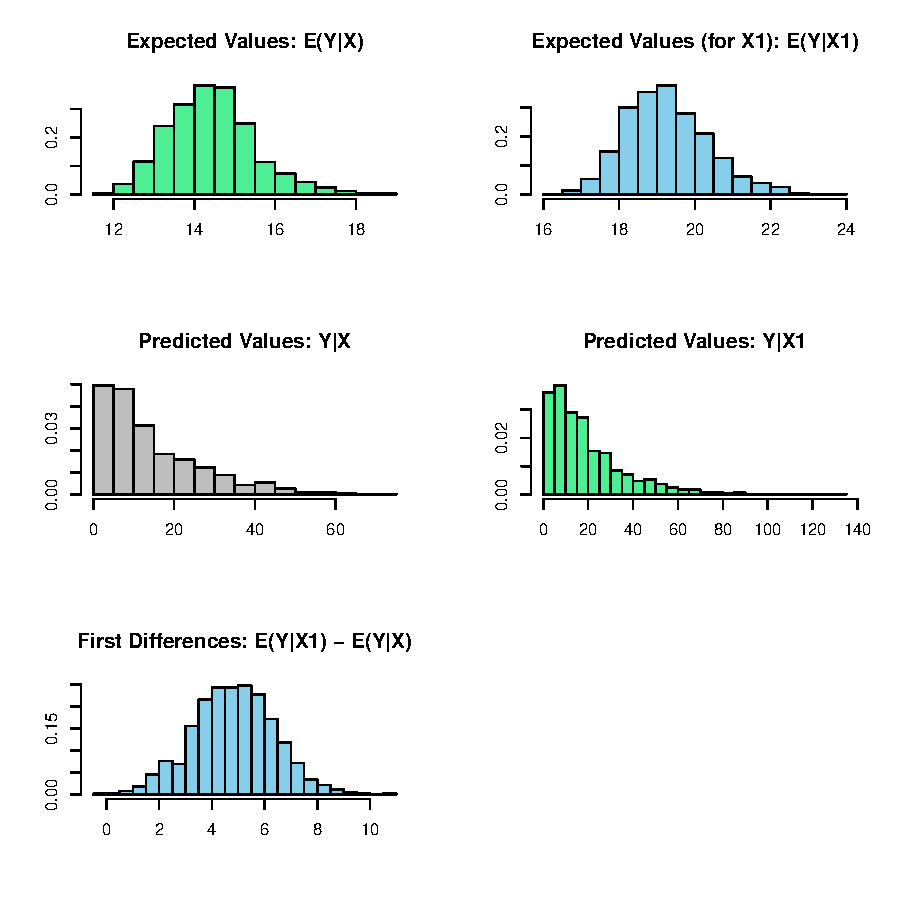
\includegraphics{vigpics/gamma-ExamplePlot}
\end{center}

\subsubsection{Model}

\begin{itemize}
\item The Gamma distribution with scale parameter $\alpha$ has a
\emph{stochastic component}:
\begin{eqnarray*}
Y &\sim& \textrm{Gamma}(y_i \mid \lambda_i, \alpha) \\
f(y)  &=& \frac{1}{\alpha^{\lambda_i} \, \Gamma \lambda_i} \, y_i^{\lambda_i
  - 1} \exp -\left\{ \frac{y_i}{\alpha} \right\}
\end{eqnarray*}
for $\alpha, \lambda_i, y_i > 0$.  \\

\item The \emph{systematic component} is given by
\begin{equation*}
  \lambda_i = \frac{1}{x_i \beta}
\end{equation*}
\end{itemize}

\subsubsection{Quantities of Interest}

\begin{itemize}
\item The expected values ({\tt qi\$ev}) are simulations of the mean
  of the stochastic component given draws of $\alpha$ and
  $\beta$ from their posteriors:  $$E(Y) = \alpha \lambda_i.$$  
\item The predicted values ({\tt qi\$pr}) are draws from the gamma
  distribution for each given set of parameters $(\alpha, \lambda_i)$.
\item If {\tt x1} is specified, {\tt sim()} also returns the
  differences in the expected values ({\tt qi\$fd}), $$E(Y \mid x_1) -
  E(Y \mid x)$$.

\item In conditional prediction models, the average expected treatment
  effect ({\tt att.ev}) for the treatment group is 
    \begin{equation*} \frac{1}{\sum_{i=1}^n t_i}\sum_{i:t_i=1}^n \left\{ Y_i(t_i=1) -
      E[Y_i(t_i=0)] \right\},
    \end{equation*} 
    where $t_i$ is a binary explanatory variable defining the treatment
    ($t_i=1$) and control ($t_i=0$) groups.  Variation in the
    simulations are due to uncertainty in simulating $E[Y_i(t_i=0)]$,
    the counterfactual expected value of $Y_i$ for observations in the
    treatment group, under the assumption that everything stays the
    same except that the treatment indicator is switched to $t_i=0$.

\item In conditional prediction models, the average predicted treatment
  effect ({\tt att.pr}) for the treatment group is 
    \begin{equation*} \frac{1}{\sum_{i=1}^n t_i}\sum_{i:t_i=1}^n \left\{ Y_i(t_i=1) -
      \widehat{Y_i(t_i=0)} \right\},
    \end{equation*} 
    where $t_i$ is a binary explanatory variable defining the treatment
    ($t_i=1$) and control ($t_i=0$) groups.  Variation in the
    simulations are due to uncertainty in simulating
    $\widehat{Y_i(t_i=0)}$, the counterfactual predicted value of
    $Y_i$ for observations in the treatment group, under the
    assumption that everything stays the same except that the
    treatment indicator is switched to $t_i=0$.  

\end{itemize}

\subsubsection{Output Values}

The output of each Zelig command contains useful information which you
may view.  For example, if you run \texttt{z.out <- zelig(y \~\,
  x, model = "gamma", data)}, then you may examine the available
information in \texttt{z.out} by using \texttt{names(z.out)},
see the {\tt coefficients} by using {\tt z.out\$coefficients}, and
a default summary of information through \texttt{summary(z.out)}.
Other elements available through the {\tt \$} operator are listed
below.

\begin{itemize}
\item From the {\tt zelig()} output object {\tt z.out}, you may
  extract:
   \begin{itemize}
   \item {\tt coefficients}: parameter estimates for the explanatory
     variables.
   \item {\tt residuals}: the working residuals in the final iteration
     of the IWLS fit.
   \item {\tt fitted.values}: the vector of fitted values.
   \item {\tt linear.predictors}: the vector of $x_{i}\beta$.
   \item {\tt aic}: Akaike's Information Criterion (minus twice the
     maximized log-likelihood plus twice the number of coefficients).
   \item {\tt df.residual}: the residual degrees of freedom.
   \item {\tt df.null}: the residual degrees of freedom for the null
     model.
   \item {\tt zelig.data}: the input data frame if {\tt save.data = TRUE}.  
   \end{itemize}

\item From {\tt summary(z.out)}, you may extract: 
   \begin{itemize}
   \item {\tt coefficients}: the parameter estimates with their
     associated standard errors, $p$-values, and $t$-statistics.
   \item{\tt cov.scaled}: a $k \times k$ matrix of scaled covariances.
   \item{\tt cov.unscaled}: a $k \times k$ matrix of unscaled
     covariances.  
   \end{itemize}

\item From the {\tt sim()} output object {\tt s.out}, you may extract
  quantities of interest arranged as matrices indexed by simulation
  $\times$ {\tt x}-observation (for more than one {\tt x}-observation).
  Available quantities are:

   \begin{itemize}
   \item {\tt qi\$ev}: the simulated expected values for the specified
     values of {\tt x}.
   \item {\tt qi\$pr}: the simulated predicted values drawn from a
     distribution defined by $(\alpha, \lambda_i)$.
   \item {\tt qi\$fd}: the simulated first difference in the expected
     values for the specified values in {\tt x} and {\tt x1}.
   \item {\tt qi\$att.ev}: the simulated average expected treatment
     effect for the treated from conditional prediction models.  
   \item {\tt qi\$att.pr}: the simulated average predicted treatment
     effect for the treated from conditional prediction models.  
   \end{itemize}
\end{itemize}


\subsection* {How to Cite} 


\CiteZelig

\subsection* {See also}
The gamma model is part of the stats package by \citet{VenRip02}.
Advanced users may wish to refer to \texttt{help(glm)} and
\texttt{help(family)}, as well as \cite{McCNel89}. Robust standard
errors are implemented via the sandwich package by \citet{Zeileis04}.
Sample data are from \cite{KinTomWit00}.

\bibliographystyle{asa}
\bibliography{gk,gkpubs}
 \end{document}


%%% Local Variables: 
%%% mode: latex
%%% TeX-master: t
%%% End: 











\documentclass[oneside,letterpaper,12pt]{book}
\usepackage{Rd}
%\usepackage{Sweave}
%\usepackage{/usr/lib64/R/share/texmf/Sweave}
%\usepackage{/usr/share/R/texmf/Sweave}
\usepackage{bibentry}
\usepackage{upquote}
\usepackage{graphicx}
\usepackage{natbib}
\usepackage[reqno]{amsmath}
\usepackage{amssymb}
\usepackage{amsfonts}
\usepackage{amsmath}
\usepackage{verbatim}
\usepackage{epsf}
\usepackage{url}
\usepackage{html}
\usepackage{dcolumn}
\usepackage{multirow}
\usepackage{fullpage}
\usepackage{lscape}
\usepackage[all]{xy}

\usepackage{csquotes}
% \usepackage[pdftex, bookmarksopen=true,bookmarksnumbered=true,
%   linkcolor=webred]{hyperref}
\bibpunct{(}{)}{;}{a}{}{,}
\newcolumntype{.}{D{.}{.}{-1}}
\newcolumntype{d}[1]{D{.}{.}{#1}}
\htmladdtonavigation{
  \htmladdnormallink{%
    \htmladdimg{http://gking.harvard.edu/pics/home.gif}}
  {http://gking.harvard.edu/}}
\newcommand{\MatchIt}{{\sc MatchIt}}
\newcommand{\hlink}{\htmladdnormallink}
\newcommand{\Sref}[1]{Section~\ref{#1}}
\newcommand{\fullrvers}{2.5.1}
\newcommand{\rvers}{2.5}
\newcommand{\rwvers}{R-2.5.1}
%\renewcommand{\bibentry}{\citealt}

\bodytext{ BACKGROUND="http://gking.harvard.edu/pics/temple.jpg"}
\setcounter{tocdepth}{2}

%\VignetteIndexEntry{Logistic Regression for Dichotomous Dependent Variables}
%\VignetteDepends{Zelig, stats}
%\VignetteKeyWords{model,logistic,dichotomous, regression}
%\VignettePackage{Zelig}
\usepackage{Sweave}
\begin{document}
\nobibliography*


\section{{\tt logit}: Logistic Regression for Dichotomous Dependent
Variables}\label{logit}

Logistic regression specifies a dichotomous dependent variable as a
function of a set of explanatory variables.  For a Bayesian
implementation, see \Sref{logit.bayes}.  

\subsubsection{Syntax}

\begin{verbatim}
> z.out <- zelig(Y ~ X1 + X2, model = "logit", data = mydata)
> x.out <- setx(z.out)
> s.out <- sim(z.out, x = x.out, x1 = NULL)
\end{verbatim}

\subsubsection{Additional Inputs} 

In addition to the standard inputs, {\tt zelig()} takes the following
additional options for logistic regression:  
\begin{itemize}
\item {\tt robust}: defaults to {\tt FALSE}.  If {\tt TRUE} is
selected, {\tt zelig()} computes robust standard errors via the {\tt
sandwich} package (see \cite{Zeileis04}).  The default type of robust
standard error is heteroskedastic and autocorrelation consistent (HAC),
and assumes that observations are ordered by time index.

In addition, {\tt robust} may be a list with the following options:  
\begin{itemize}
\item {\tt method}:  Choose from 
\begin{itemize}
\item {\tt "vcovHAC"}: (default if {\tt robust = TRUE}) HAC standard
errors. 
\item {\tt "kernHAC"}: HAC standard errors using the
weights given in \cite{Andrews91}. 
\item {\tt "weave"}: HAC standard errors using the
weights given in \cite{LumHea99}.  
\end{itemize}  
\item {\tt order.by}: defaults to {\tt NULL} (the observations are
chronologically ordered as in the original data).  Optionally, you may
specify a vector of weights (either as {\tt order.by = z}, where {\tt
z} exists outside the data frame; or as {\tt order.by = \~{}z}, where
{\tt z} is a variable in the data frame)  The observations are
chronologically ordered by the size of {\tt z}.
\item {\tt \dots}:  additional options passed to the functions 
specified in {\tt method}.   See the {\tt sandwich} library and
\cite{Zeileis04} for more options.   
\end{itemize}
\end{itemize}

\subsubsection{Examples}
\begin{enumerate}
\item {Basic Example}
 
Attaching the sample turnout dataset:
\begin{Schunk}
\begin{Sinput}
> data(turnout)
\end{Sinput}
\end{Schunk}
Estimating parameter values for the logistic regression:
\begin{Schunk}
\begin{Sinput}
> z.out1 <- zelig(vote ~ age + race, model = "logit", data = turnout)
\end{Sinput}
\end{Schunk}
Setting values for the explanatory variables:
\begin{Schunk}
\begin{Sinput}
> x.out1 <- setx(z.out1, age = 36, race = "white")
\end{Sinput}
\end{Schunk}
Simulating quantities of interest from the posterior distribution.
\begin{Schunk}
\begin{Sinput}
> s.out1 <- sim(z.out1, x = x.out1)
\end{Sinput}
\end{Schunk}
\begin{Schunk}
\begin{Sinput}
> summary(s.out1)
\end{Sinput}
\end{Schunk}
\begin{center}
\begin{Schunk}
\begin{Sinput}
> plot(s.out1)
\end{Sinput}
\end{Schunk}
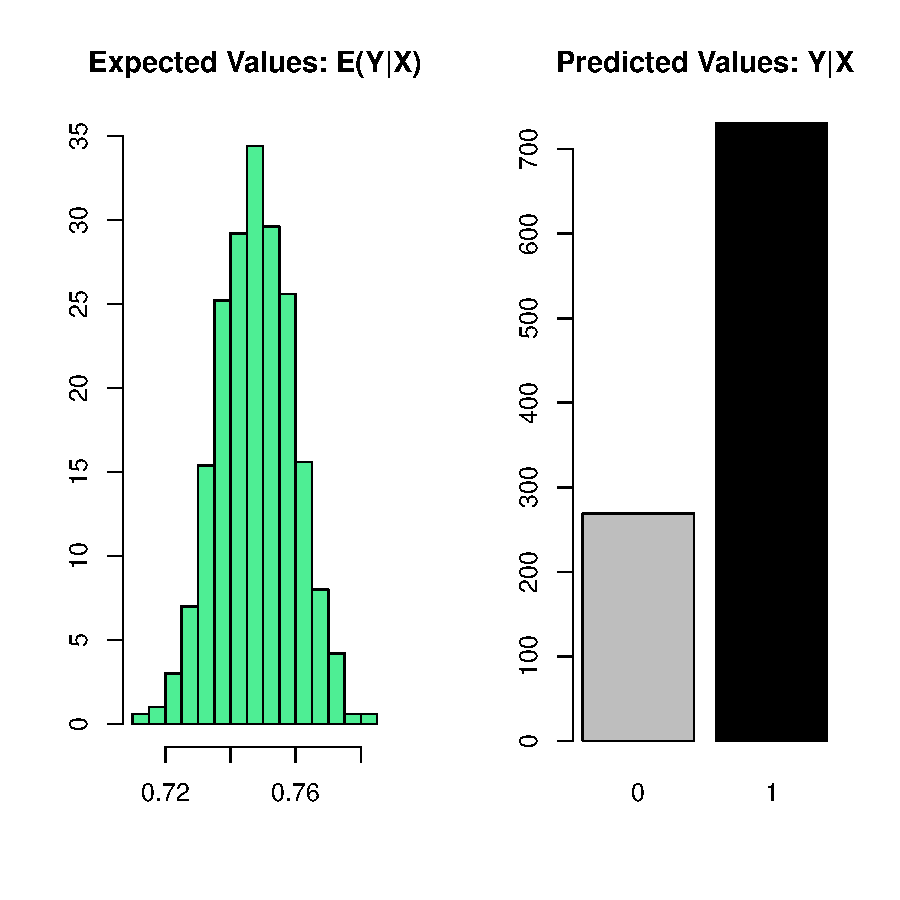
\includegraphics{vigpics/logit-ExamplePlot}
\end{center}

\item {Simulating First Differences}

Estimating the risk difference (and risk ratio) between low education
(25th percentile) and high education (75th percentile) while all the
other variables held at their default values.
\begin{Schunk}
\begin{Sinput}
> z.out2 <- zelig(vote ~ race + educate, model = "logit", data = turnout)
> x.high <- setx(z.out2, educate = quantile(turnout$educate, prob = 0.75))
> x.low <- setx(z.out2, educate = quantile(turnout$educate, prob = 0.25))
\end{Sinput}
\end{Schunk}

\begin{Schunk}
\begin{Sinput}
> s.out2 <- sim(z.out2, x = x.high, x1 = x.low)
\end{Sinput}
\end{Schunk}
\begin{Schunk}
\begin{Sinput}
> summary(s.out2)
\end{Sinput}
\end{Schunk}
\begin{center}
\begin{Schunk}
\begin{Sinput}
> plot(s.out2)
\end{Sinput}
\end{Schunk}
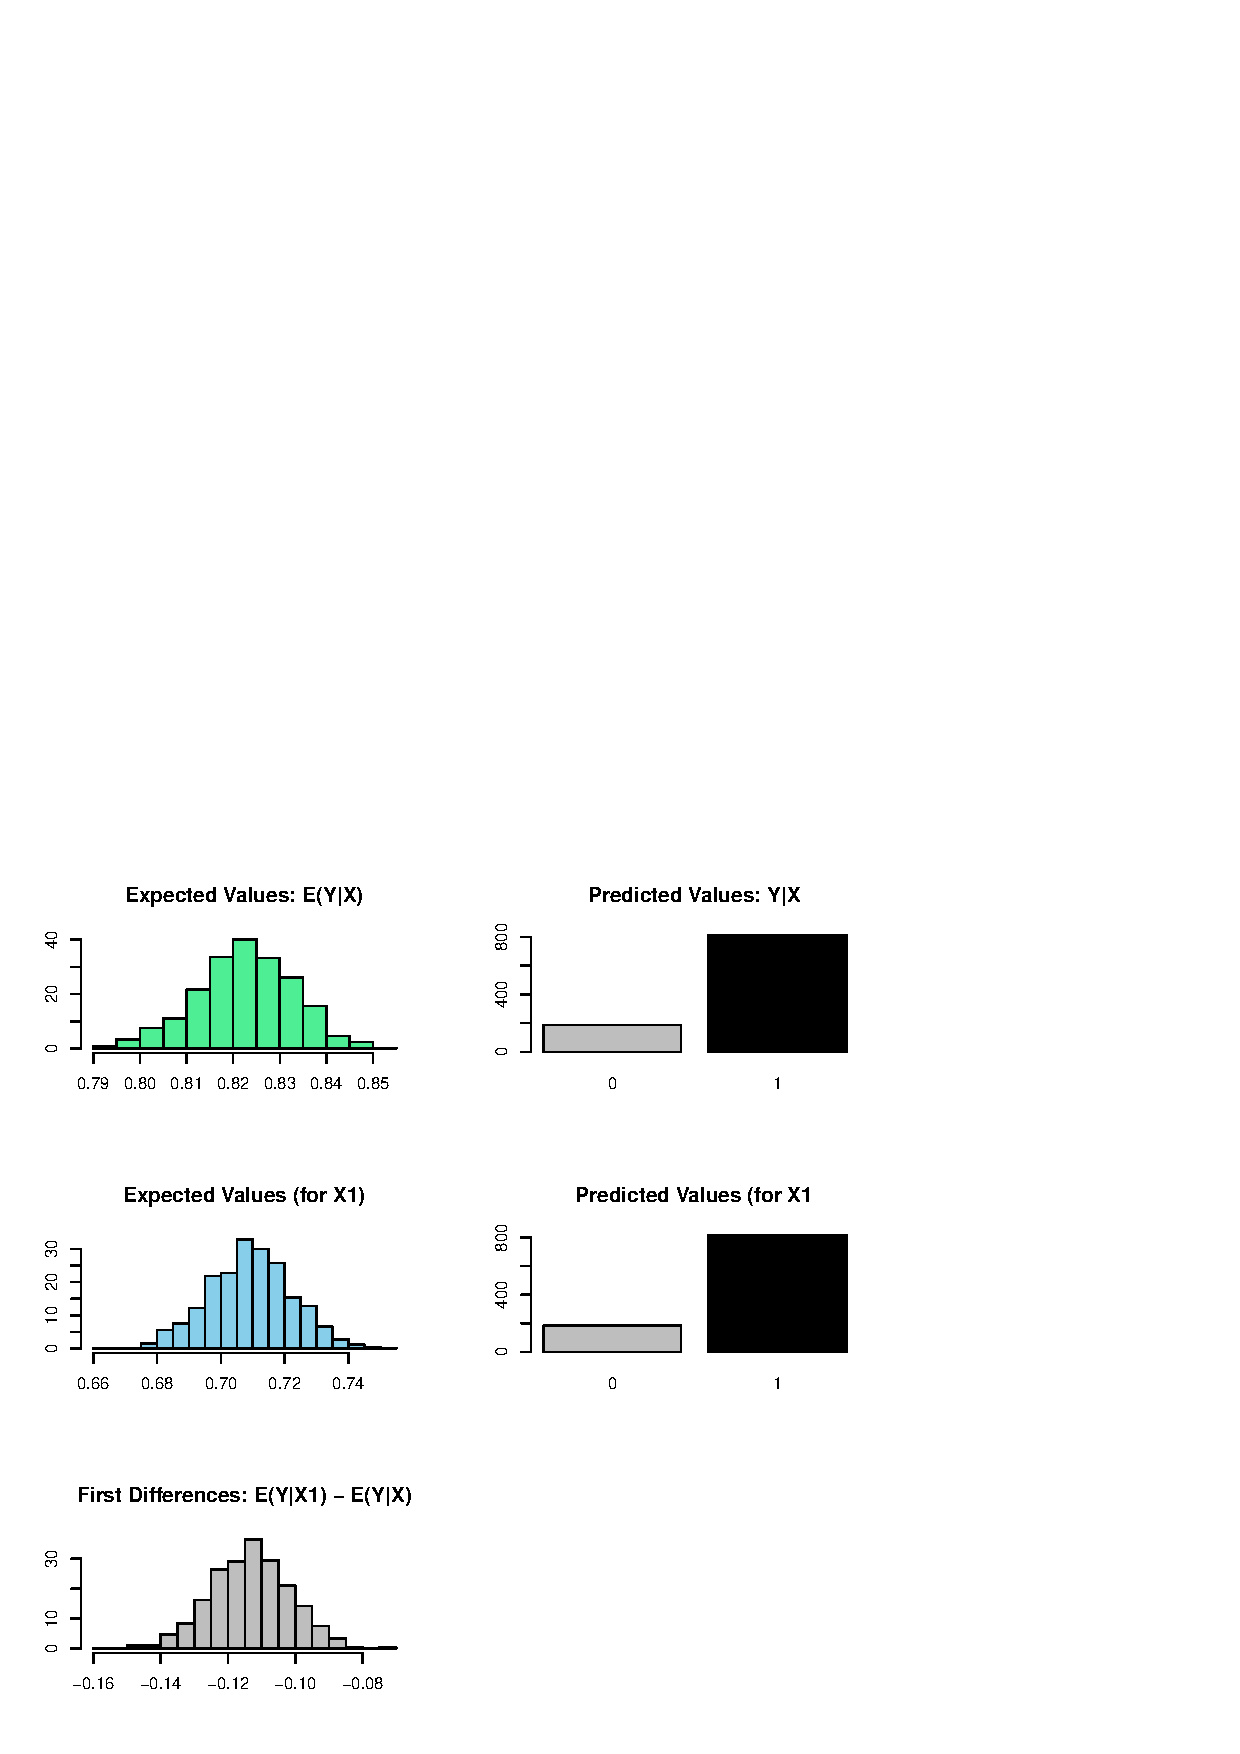
\includegraphics{vigpics/logit-FirstDifferencesPlot}
\end{center} 


\item {Presenting Results: An ROC Plot}  \label{ROC}
  
  One can use an ROC plot to evaluate the fit of alternative model
  specifications.  (Use {\tt demo(roc)} to view this example, or see
  King and Zeng (2002)\nocite{KinZen02}.)  
\begin{Schunk}
\begin{Sinput}
> z.out1 <- zelig(vote ~ race + educate + age, model = "logit", 
+     data = turnout)
> z.out2 <- zelig(vote ~ race + educate, model = "logit", data = turnout)
\end{Sinput}
\end{Schunk}
\begin{center}
\begin{Schunk}
\begin{Sinput}
> rocplot(z.out1$y, z.out2$y, fitted(z.out1), fitted(z.out2))
\end{Sinput}
\end{Schunk}
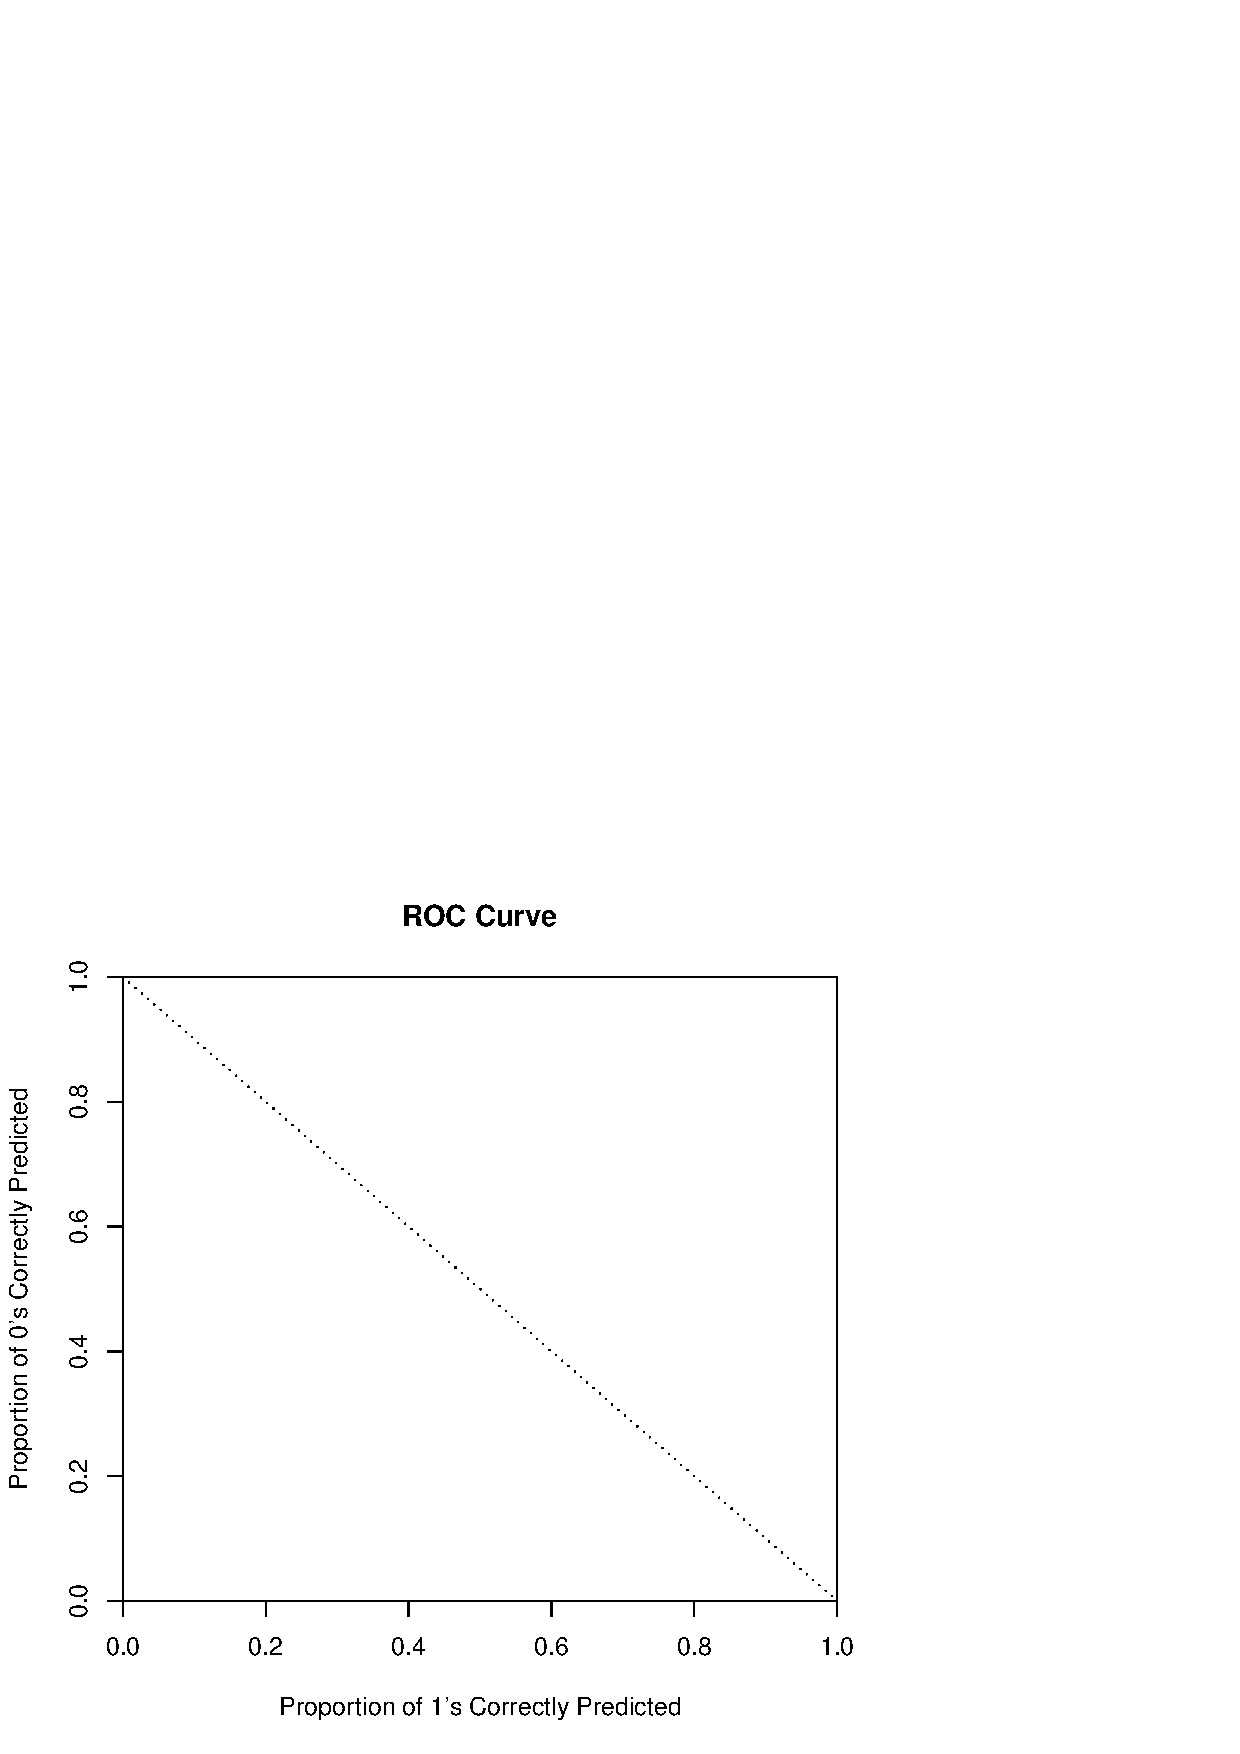
\includegraphics{vigpics/logit-ROCPlot}
\end{center}
\end{enumerate}

\subsubsection{Model}
Let $Y_i$ be the binary dependent variable for observation $i$ which
takes the value of either 0 or 1.
\begin{itemize}

\item The \emph{stochastic component} is given by  
\begin{eqnarray*}
Y_i &\sim& \textrm{Bernoulli}(y_i \mid \pi_i) \\
    &=& \pi_i^{y_i} (1-\pi_i)^{1-y_i}
\end{eqnarray*}
where $\pi_i=\Pr(Y_i=1)$.

\item The \emph{systematic component} is given by: 
\begin{equation*}
\pi_i \; = \; \frac{1}{1 + \exp(-x_i \beta)}.
\end{equation*}
where $x_i$ is the vector of $k$ explanatory variables for observation $i$
and $\beta$ is the vector of coefficients.
\end{itemize}

\subsubsection{Quantities of Interest}
\begin{itemize}
\item The expected values ({\tt qi\$ev}) for the logit model are
  simulations of the predicted probability of a success: $$E(Y) =
  \pi_i= \frac{1}{1 + \exp(-x_i \beta)},$$ given draws of $\beta$ from
  its sampling distribution.

\item The predicted values ({\tt qi\$pr}) are draws from the Binomial
  distribution with mean equal to the simulated expected value $\pi_i$.  

\item The first difference ({\tt qi\$fd}) for the logit model is defined as
\begin{equation*}
\textrm{FD} = \Pr(Y = 1 \mid x_1) - \Pr(Y = 1 \mid x).
\end{equation*}

\item The risk ratio ({\tt qi\$rr}) is defined as
\begin{equation*}
\textrm{RR} = \Pr(Y = 1 \mid x_1) \ / \ \Pr(Y = 1 \mid x).
\end{equation*}

\item In conditional prediction models, the average expected treatment
  effect ({\tt att.ev}) for the treatment group is 
    \begin{equation*} \frac{1}{\sum_{i=1}^n t_i}\sum_{i:t_i=1}^n \left\{ Y_i(t_i=1) -
      E[Y_i(t_i=0)] \right\},
    \end{equation*} 
    where $t_i$ is a binary explanatory variable defining the treatment
    ($t_i=1$) and control ($t_i=0$) groups.  Variation in the
    simulations are due to uncertainty in simulating $E[Y_i(t_i=0)]$,
    the counterfactual expected value of $Y_i$ for observations in the
    treatment group, under the assumption that everything stays the
    same except that the treatment indicator is switched to $t_i=0$.

\item In conditional prediction models, the average predicted treatment
  effect ({\tt att.pr}) for the treatment group is 
    \begin{equation*} \frac{1}{\sum_{i=1}^n t_i}\sum_{i:t_i=1}^n \left\{ Y_i(t_i=1) -
      \widehat{Y_i(t_i=0)}\right\},
    \end{equation*} 
    where $t_i$ is a binary explanatory variable defining the
    treatment ($t_i=1$) and control ($t_i=0$) groups.  Variation in
    the simulations are due to uncertainty in simulating
    $\widehat{Y_i(t_i=0)}$, the counterfactual predicted value of
    $Y_i$ for observations in the treatment group, under the
    assumption that everything stays the same except that the
    treatment indicator is switched to $t_i=0$.
\end{itemize}

\subsubsection{Output Values}

The output of each Zelig command contains useful information which you
may view.  For example, if you run \texttt{z.out <- zelig(y \~\, x,
  model = "logit", data)}, then you may examine the available
information in \texttt{z.out} by using \texttt{names(z.out)},
see the {\tt coefficients} by using {\tt z.out\$coefficients}, and
a default summary of information through \texttt{summary(z.out)}.
Other elements available through the {\tt \$} operator are listed
below.

\begin{itemize}
\item From the {\tt zelig()} output object {\tt z.out}, you may
  extract:
   \begin{itemize}
   \item {\tt coefficients}: parameter estimates for the explanatory
     variables.
   \item {\tt residuals}: the working residuals in the final iteration
     of the IWLS fit.
   \item {\tt fitted.values}: the vector of fitted values for the
     systemic component, $\pi_i$.
   \item {\tt linear.predictors}: the vector of $x_{i}\beta$
   \item {\tt aic}: Akaike's Information Criterion (minus twice the
     maximized log-likelihood plus twice the number of coefficients).
   \item {\tt df.residual}: the residual degrees of freedom.
   \item {\tt df.null}: the residual degrees of freedom for the null
     model.
   \item {\tt data}: the name of the input data frame.  
   \end{itemize}

\item From {\tt summary(z.out)}, you may extract: 
   \begin{itemize}
   \item {\tt coefficients}: the parameter estimates with their
     associated standard errors, $p$-values, and $t$-statistics.
   \item{\tt cov.scaled}: a $k \times k$ matrix of scaled covariances.
   \item{\tt cov.unscaled}: a $k \times k$ matrix of unscaled
     covariances.  
   \end{itemize}

\item From the {\tt sim()} output object {\tt s.out}, you may extract
  quantities of interest arranged as matrices indexed by simulation
  $\times$ {\tt x}-observation (for more than one {\tt x}-observation).
  Available quantities are:

   \begin{itemize}
   \item {\tt qi\$ev}: the simulated expected probabilities for the
     specified values of {\tt x}.
   \item {\tt qi\$pr}: the simulated predicted values for the
     specified values of {\tt x}.
   \item {\tt qi\$fd}: the simulated first difference in the expected
     probabilities for the values specified in {\tt x} and {\tt x1}.
   \item {\tt qi\$rr}: the simulated risk ratio for the expected
     probabilities simulated from {\tt x} and {\tt x1}.
   \item {\tt qi\$att.ev}: the simulated average expected treatment
     effect for the treated from conditional prediction models.  
   \item {\tt qi\$att.pr}: the simulated average predicted treatment
     effect for the treated from conditional prediction models.  
   \end{itemize}
\end{itemize}

\subsection* {How to Cite} 


\documentclass[oneside,letterpaper,12pt]{book}
\usepackage{Rd}
%\usepackage{Sweave}
%\usepackage{/usr/lib64/R/share/texmf/Sweave}
%\usepackage{/usr/share/R/texmf/Sweave}
\usepackage{bibentry}
\usepackage{upquote}
\usepackage{graphicx}
\usepackage{natbib}
\usepackage[reqno]{amsmath}
\usepackage{amssymb}
\usepackage{amsfonts}
\usepackage{amsmath}
\usepackage{verbatim}
\usepackage{epsf}
\usepackage{url}
\usepackage{html}
\usepackage{dcolumn}
\usepackage{multirow}
\usepackage{fullpage}
\usepackage{lscape}
\usepackage[all]{xy}

\usepackage{csquotes}
% \usepackage[pdftex, bookmarksopen=true,bookmarksnumbered=true,
%   linkcolor=webred]{hyperref}
\bibpunct{(}{)}{;}{a}{}{,}
\newcolumntype{.}{D{.}{.}{-1}}
\newcolumntype{d}[1]{D{.}{.}{#1}}
\htmladdtonavigation{
  \htmladdnormallink{%
    \htmladdimg{http://gking.harvard.edu/pics/home.gif}}
  {http://gking.harvard.edu/}}
\newcommand{\MatchIt}{{\sc MatchIt}}
\newcommand{\hlink}{\htmladdnormallink}
\newcommand{\Sref}[1]{Section~\ref{#1}}
\newcommand{\fullrvers}{2.5.1}
\newcommand{\rvers}{2.5}
\newcommand{\rwvers}{R-2.5.1}
%\renewcommand{\bibentry}{\citealt}

\bodytext{ BACKGROUND="http://gking.harvard.edu/pics/temple.jpg"}
\setcounter{tocdepth}{2}

%\VignetteIndexEntry{Logistic Regression for Dichotomous Dependent Variables}
%\VignetteDepends{Zelig, stats}
%\VignetteKeyWords{model,logistic,dichotomous, regression}
%\VignettePackage{Zelig}
\usepackage{Sweave}
\begin{document}
\nobibliography*


\section{{\tt logit}: Logistic Regression for Dichotomous Dependent
Variables}\label{logit}

Logistic regression specifies a dichotomous dependent variable as a
function of a set of explanatory variables.  For a Bayesian
implementation, see \Sref{logit.bayes}.  

\subsubsection{Syntax}

\begin{verbatim}
> z.out <- zelig(Y ~ X1 + X2, model = "logit", data = mydata)
> x.out <- setx(z.out)
> s.out <- sim(z.out, x = x.out, x1 = NULL)
\end{verbatim}

\subsubsection{Additional Inputs} 

In addition to the standard inputs, {\tt zelig()} takes the following
additional options for logistic regression:  
\begin{itemize}
\item {\tt robust}: defaults to {\tt FALSE}.  If {\tt TRUE} is
selected, {\tt zelig()} computes robust standard errors via the {\tt
sandwich} package (see \cite{Zeileis04}).  The default type of robust
standard error is heteroskedastic and autocorrelation consistent (HAC),
and assumes that observations are ordered by time index.

In addition, {\tt robust} may be a list with the following options:  
\begin{itemize}
\item {\tt method}:  Choose from 
\begin{itemize}
\item {\tt "vcovHAC"}: (default if {\tt robust = TRUE}) HAC standard
errors. 
\item {\tt "kernHAC"}: HAC standard errors using the
weights given in \cite{Andrews91}. 
\item {\tt "weave"}: HAC standard errors using the
weights given in \cite{LumHea99}.  
\end{itemize}  
\item {\tt order.by}: defaults to {\tt NULL} (the observations are
chronologically ordered as in the original data).  Optionally, you may
specify a vector of weights (either as {\tt order.by = z}, where {\tt
z} exists outside the data frame; or as {\tt order.by = \~{}z}, where
{\tt z} is a variable in the data frame)  The observations are
chronologically ordered by the size of {\tt z}.
\item {\tt \dots}:  additional options passed to the functions 
specified in {\tt method}.   See the {\tt sandwich} library and
\cite{Zeileis04} for more options.   
\end{itemize}
\end{itemize}

\subsubsection{Examples}
\begin{enumerate}
\item {Basic Example}
 
Attaching the sample turnout dataset:
\begin{Schunk}
\begin{Sinput}
> data(turnout)
\end{Sinput}
\end{Schunk}
Estimating parameter values for the logistic regression:
\begin{Schunk}
\begin{Sinput}
> z.out1 <- zelig(vote ~ age + race, model = "logit", data = turnout)
\end{Sinput}
\end{Schunk}
Setting values for the explanatory variables:
\begin{Schunk}
\begin{Sinput}
> x.out1 <- setx(z.out1, age = 36, race = "white")
\end{Sinput}
\end{Schunk}
Simulating quantities of interest from the posterior distribution.
\begin{Schunk}
\begin{Sinput}
> s.out1 <- sim(z.out1, x = x.out1)
\end{Sinput}
\end{Schunk}
\begin{Schunk}
\begin{Sinput}
> summary(s.out1)
\end{Sinput}
\end{Schunk}
\begin{center}
\begin{Schunk}
\begin{Sinput}
> plot(s.out1)
\end{Sinput}
\end{Schunk}
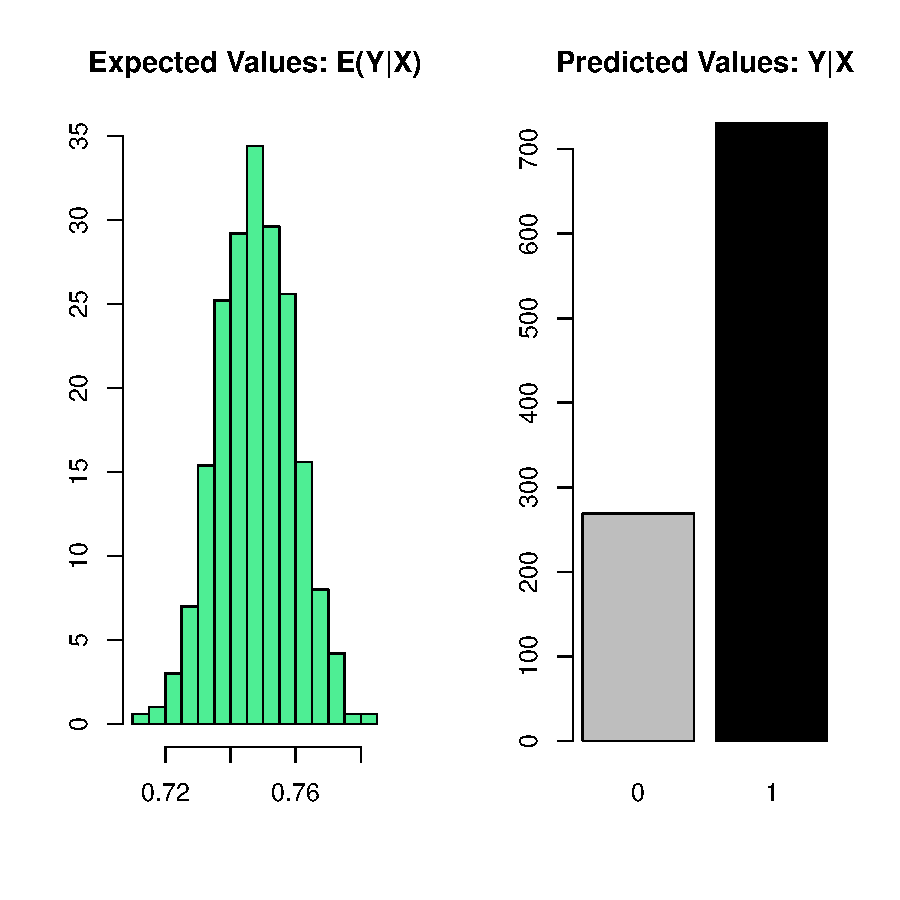
\includegraphics{vigpics/logit-ExamplePlot}
\end{center}

\item {Simulating First Differences}

Estimating the risk difference (and risk ratio) between low education
(25th percentile) and high education (75th percentile) while all the
other variables held at their default values.
\begin{Schunk}
\begin{Sinput}
> z.out2 <- zelig(vote ~ race + educate, model = "logit", data = turnout)
> x.high <- setx(z.out2, educate = quantile(turnout$educate, prob = 0.75))
> x.low <- setx(z.out2, educate = quantile(turnout$educate, prob = 0.25))
\end{Sinput}
\end{Schunk}

\begin{Schunk}
\begin{Sinput}
> s.out2 <- sim(z.out2, x = x.high, x1 = x.low)
\end{Sinput}
\end{Schunk}
\begin{Schunk}
\begin{Sinput}
> summary(s.out2)
\end{Sinput}
\end{Schunk}
\begin{center}
\begin{Schunk}
\begin{Sinput}
> plot(s.out2)
\end{Sinput}
\end{Schunk}
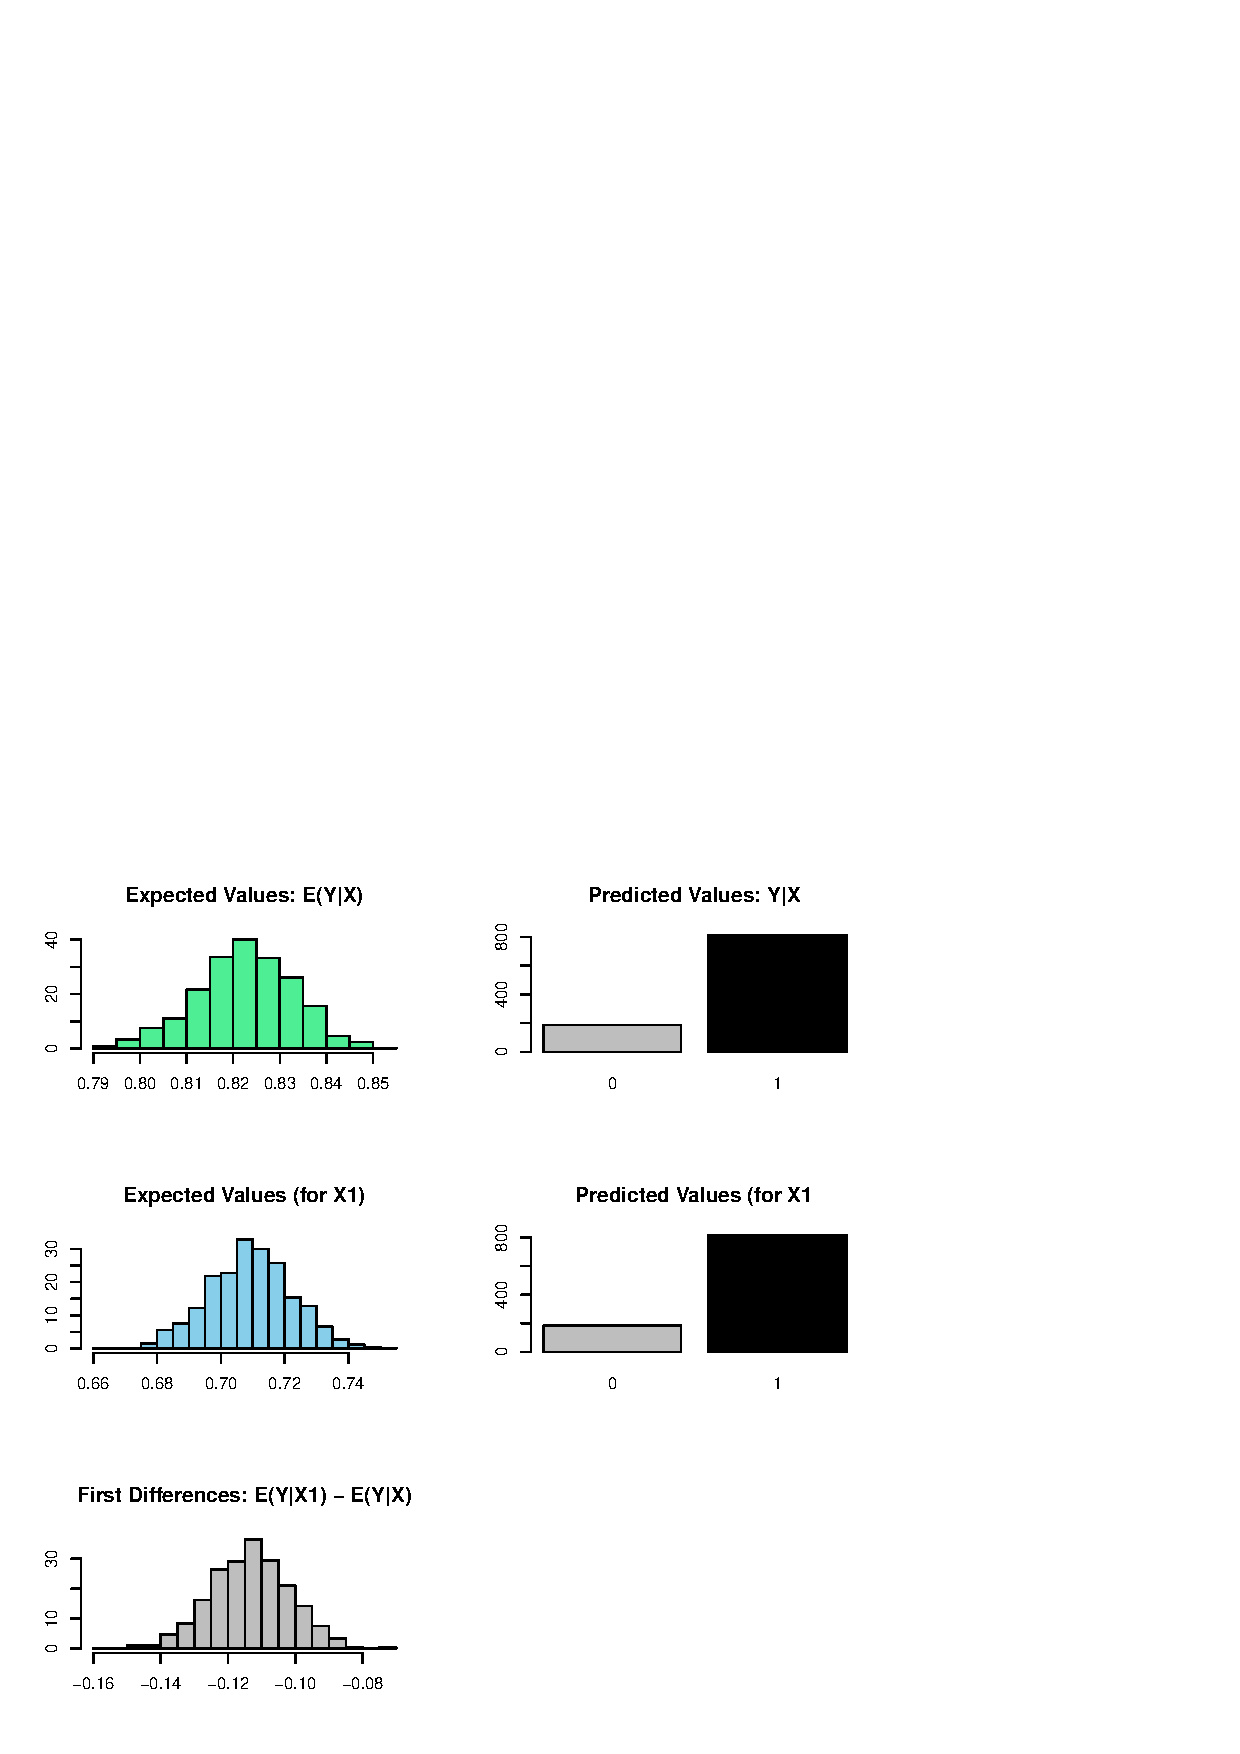
\includegraphics{vigpics/logit-FirstDifferencesPlot}
\end{center} 


\item {Presenting Results: An ROC Plot}  \label{ROC}
  
  One can use an ROC plot to evaluate the fit of alternative model
  specifications.  (Use {\tt demo(roc)} to view this example, or see
  King and Zeng (2002)\nocite{KinZen02}.)  
\begin{Schunk}
\begin{Sinput}
> z.out1 <- zelig(vote ~ race + educate + age, model = "logit", 
+     data = turnout)
> z.out2 <- zelig(vote ~ race + educate, model = "logit", data = turnout)
\end{Sinput}
\end{Schunk}
\begin{center}
\begin{Schunk}
\begin{Sinput}
> rocplot(z.out1$y, z.out2$y, fitted(z.out1), fitted(z.out2))
\end{Sinput}
\end{Schunk}
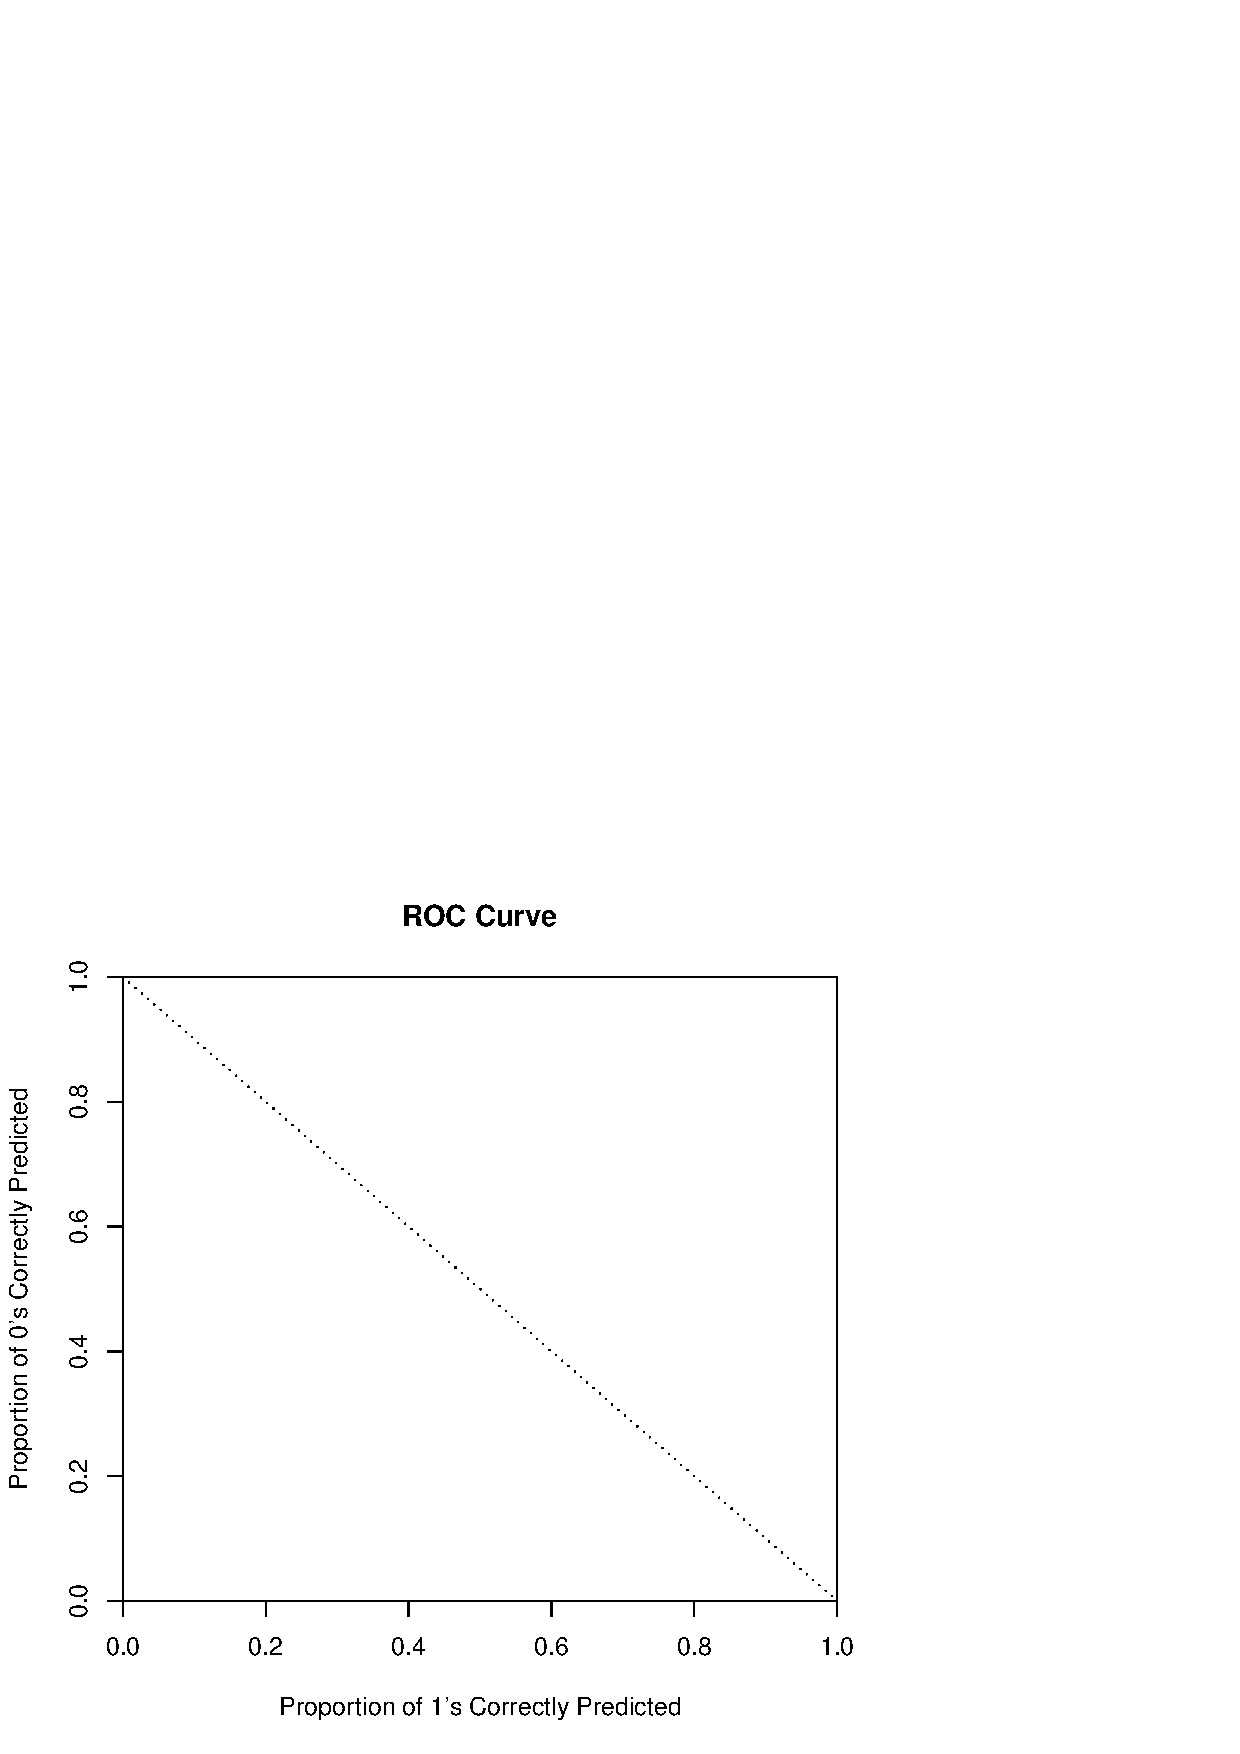
\includegraphics{vigpics/logit-ROCPlot}
\end{center}
\end{enumerate}

\subsubsection{Model}
Let $Y_i$ be the binary dependent variable for observation $i$ which
takes the value of either 0 or 1.
\begin{itemize}

\item The \emph{stochastic component} is given by  
\begin{eqnarray*}
Y_i &\sim& \textrm{Bernoulli}(y_i \mid \pi_i) \\
    &=& \pi_i^{y_i} (1-\pi_i)^{1-y_i}
\end{eqnarray*}
where $\pi_i=\Pr(Y_i=1)$.

\item The \emph{systematic component} is given by: 
\begin{equation*}
\pi_i \; = \; \frac{1}{1 + \exp(-x_i \beta)}.
\end{equation*}
where $x_i$ is the vector of $k$ explanatory variables for observation $i$
and $\beta$ is the vector of coefficients.
\end{itemize}

\subsubsection{Quantities of Interest}
\begin{itemize}
\item The expected values ({\tt qi\$ev}) for the logit model are
  simulations of the predicted probability of a success: $$E(Y) =
  \pi_i= \frac{1}{1 + \exp(-x_i \beta)},$$ given draws of $\beta$ from
  its sampling distribution.

\item The predicted values ({\tt qi\$pr}) are draws from the Binomial
  distribution with mean equal to the simulated expected value $\pi_i$.  

\item The first difference ({\tt qi\$fd}) for the logit model is defined as
\begin{equation*}
\textrm{FD} = \Pr(Y = 1 \mid x_1) - \Pr(Y = 1 \mid x).
\end{equation*}

\item The risk ratio ({\tt qi\$rr}) is defined as
\begin{equation*}
\textrm{RR} = \Pr(Y = 1 \mid x_1) \ / \ \Pr(Y = 1 \mid x).
\end{equation*}

\item In conditional prediction models, the average expected treatment
  effect ({\tt att.ev}) for the treatment group is 
    \begin{equation*} \frac{1}{\sum_{i=1}^n t_i}\sum_{i:t_i=1}^n \left\{ Y_i(t_i=1) -
      E[Y_i(t_i=0)] \right\},
    \end{equation*} 
    where $t_i$ is a binary explanatory variable defining the treatment
    ($t_i=1$) and control ($t_i=0$) groups.  Variation in the
    simulations are due to uncertainty in simulating $E[Y_i(t_i=0)]$,
    the counterfactual expected value of $Y_i$ for observations in the
    treatment group, under the assumption that everything stays the
    same except that the treatment indicator is switched to $t_i=0$.

\item In conditional prediction models, the average predicted treatment
  effect ({\tt att.pr}) for the treatment group is 
    \begin{equation*} \frac{1}{\sum_{i=1}^n t_i}\sum_{i:t_i=1}^n \left\{ Y_i(t_i=1) -
      \widehat{Y_i(t_i=0)}\right\},
    \end{equation*} 
    where $t_i$ is a binary explanatory variable defining the
    treatment ($t_i=1$) and control ($t_i=0$) groups.  Variation in
    the simulations are due to uncertainty in simulating
    $\widehat{Y_i(t_i=0)}$, the counterfactual predicted value of
    $Y_i$ for observations in the treatment group, under the
    assumption that everything stays the same except that the
    treatment indicator is switched to $t_i=0$.
\end{itemize}

\subsubsection{Output Values}

The output of each Zelig command contains useful information which you
may view.  For example, if you run \texttt{z.out <- zelig(y \~\, x,
  model = "logit", data)}, then you may examine the available
information in \texttt{z.out} by using \texttt{names(z.out)},
see the {\tt coefficients} by using {\tt z.out\$coefficients}, and
a default summary of information through \texttt{summary(z.out)}.
Other elements available through the {\tt \$} operator are listed
below.

\begin{itemize}
\item From the {\tt zelig()} output object {\tt z.out}, you may
  extract:
   \begin{itemize}
   \item {\tt coefficients}: parameter estimates for the explanatory
     variables.
   \item {\tt residuals}: the working residuals in the final iteration
     of the IWLS fit.
   \item {\tt fitted.values}: the vector of fitted values for the
     systemic component, $\pi_i$.
   \item {\tt linear.predictors}: the vector of $x_{i}\beta$
   \item {\tt aic}: Akaike's Information Criterion (minus twice the
     maximized log-likelihood plus twice the number of coefficients).
   \item {\tt df.residual}: the residual degrees of freedom.
   \item {\tt df.null}: the residual degrees of freedom for the null
     model.
   \item {\tt data}: the name of the input data frame.  
   \end{itemize}

\item From {\tt summary(z.out)}, you may extract: 
   \begin{itemize}
   \item {\tt coefficients}: the parameter estimates with their
     associated standard errors, $p$-values, and $t$-statistics.
   \item{\tt cov.scaled}: a $k \times k$ matrix of scaled covariances.
   \item{\tt cov.unscaled}: a $k \times k$ matrix of unscaled
     covariances.  
   \end{itemize}

\item From the {\tt sim()} output object {\tt s.out}, you may extract
  quantities of interest arranged as matrices indexed by simulation
  $\times$ {\tt x}-observation (for more than one {\tt x}-observation).
  Available quantities are:

   \begin{itemize}
   \item {\tt qi\$ev}: the simulated expected probabilities for the
     specified values of {\tt x}.
   \item {\tt qi\$pr}: the simulated predicted values for the
     specified values of {\tt x}.
   \item {\tt qi\$fd}: the simulated first difference in the expected
     probabilities for the values specified in {\tt x} and {\tt x1}.
   \item {\tt qi\$rr}: the simulated risk ratio for the expected
     probabilities simulated from {\tt x} and {\tt x1}.
   \item {\tt qi\$att.ev}: the simulated average expected treatment
     effect for the treated from conditional prediction models.  
   \item {\tt qi\$att.pr}: the simulated average predicted treatment
     effect for the treated from conditional prediction models.  
   \end{itemize}
\end{itemize}

\subsection* {How to Cite} 


\include{zinput}
%\VignetteIndexEntry{Logistic Regression for Dichotomous Dependent Variables}
%\VignetteDepends{Zelig, stats}
%\VignetteKeyWords{model,logistic,dichotomous, regression}
%\VignettePackage{Zelig}
\usepackage{Sweave}
\begin{document}
\nobibliography*


\section{{\tt logit}: Logistic Regression for Dichotomous Dependent
Variables}\label{logit}

Logistic regression specifies a dichotomous dependent variable as a
function of a set of explanatory variables.  For a Bayesian
implementation, see \Sref{logit.bayes}.  

\subsubsection{Syntax}

\begin{verbatim}
> z.out <- zelig(Y ~ X1 + X2, model = "logit", data = mydata)
> x.out <- setx(z.out)
> s.out <- sim(z.out, x = x.out, x1 = NULL)
\end{verbatim}

\subsubsection{Additional Inputs} 

In addition to the standard inputs, {\tt zelig()} takes the following
additional options for logistic regression:  
\begin{itemize}
\item {\tt robust}: defaults to {\tt FALSE}.  If {\tt TRUE} is
selected, {\tt zelig()} computes robust standard errors via the {\tt
sandwich} package (see \cite{Zeileis04}).  The default type of robust
standard error is heteroskedastic and autocorrelation consistent (HAC),
and assumes that observations are ordered by time index.

In addition, {\tt robust} may be a list with the following options:  
\begin{itemize}
\item {\tt method}:  Choose from 
\begin{itemize}
\item {\tt "vcovHAC"}: (default if {\tt robust = TRUE}) HAC standard
errors. 
\item {\tt "kernHAC"}: HAC standard errors using the
weights given in \cite{Andrews91}. 
\item {\tt "weave"}: HAC standard errors using the
weights given in \cite{LumHea99}.  
\end{itemize}  
\item {\tt order.by}: defaults to {\tt NULL} (the observations are
chronologically ordered as in the original data).  Optionally, you may
specify a vector of weights (either as {\tt order.by = z}, where {\tt
z} exists outside the data frame; or as {\tt order.by = \~{}z}, where
{\tt z} is a variable in the data frame)  The observations are
chronologically ordered by the size of {\tt z}.
\item {\tt \dots}:  additional options passed to the functions 
specified in {\tt method}.   See the {\tt sandwich} library and
\cite{Zeileis04} for more options.   
\end{itemize}
\end{itemize}

\subsubsection{Examples}
\begin{enumerate}
\item {Basic Example}
 
Attaching the sample turnout dataset:
\begin{Schunk}
\begin{Sinput}
> data(turnout)
\end{Sinput}
\end{Schunk}
Estimating parameter values for the logistic regression:
\begin{Schunk}
\begin{Sinput}
> z.out1 <- zelig(vote ~ age + race, model = "logit", data = turnout)
\end{Sinput}
\end{Schunk}
Setting values for the explanatory variables:
\begin{Schunk}
\begin{Sinput}
> x.out1 <- setx(z.out1, age = 36, race = "white")
\end{Sinput}
\end{Schunk}
Simulating quantities of interest from the posterior distribution.
\begin{Schunk}
\begin{Sinput}
> s.out1 <- sim(z.out1, x = x.out1)
\end{Sinput}
\end{Schunk}
\begin{Schunk}
\begin{Sinput}
> summary(s.out1)
\end{Sinput}
\end{Schunk}
\begin{center}
\begin{Schunk}
\begin{Sinput}
> plot(s.out1)
\end{Sinput}
\end{Schunk}
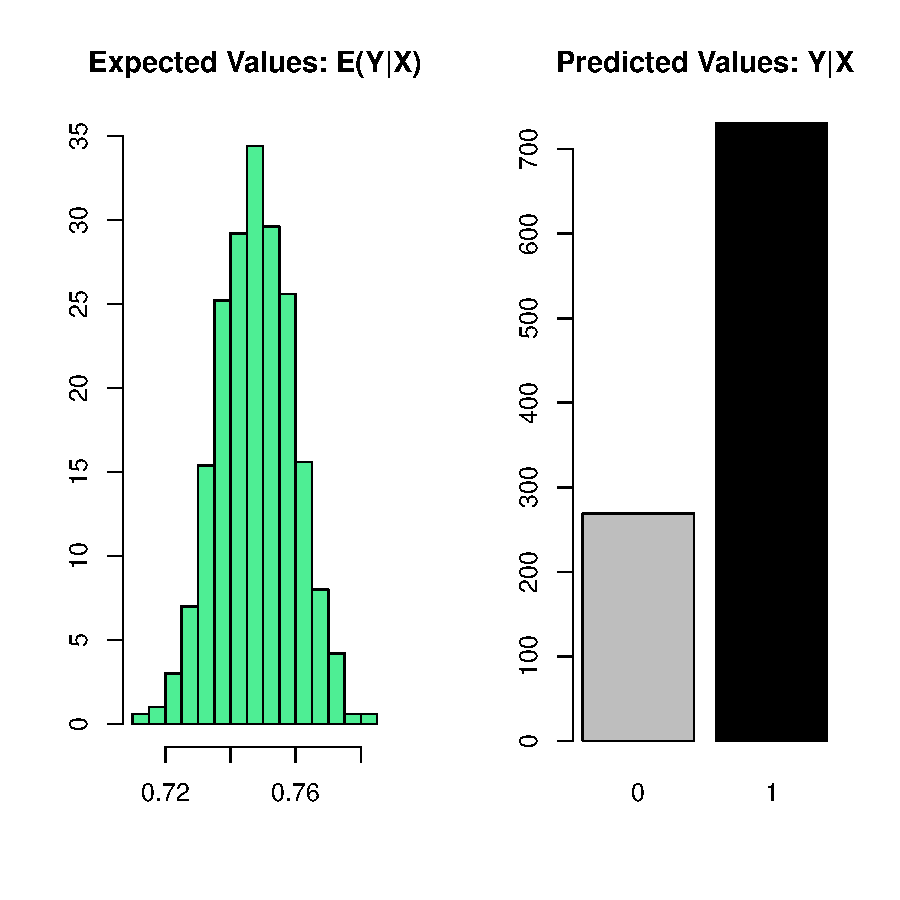
\includegraphics{vigpics/logit-ExamplePlot}
\end{center}

\item {Simulating First Differences}

Estimating the risk difference (and risk ratio) between low education
(25th percentile) and high education (75th percentile) while all the
other variables held at their default values.
\begin{Schunk}
\begin{Sinput}
> z.out2 <- zelig(vote ~ race + educate, model = "logit", data = turnout)
> x.high <- setx(z.out2, educate = quantile(turnout$educate, prob = 0.75))
> x.low <- setx(z.out2, educate = quantile(turnout$educate, prob = 0.25))
\end{Sinput}
\end{Schunk}

\begin{Schunk}
\begin{Sinput}
> s.out2 <- sim(z.out2, x = x.high, x1 = x.low)
\end{Sinput}
\end{Schunk}
\begin{Schunk}
\begin{Sinput}
> summary(s.out2)
\end{Sinput}
\end{Schunk}
\begin{center}
\begin{Schunk}
\begin{Sinput}
> plot(s.out2)
\end{Sinput}
\end{Schunk}
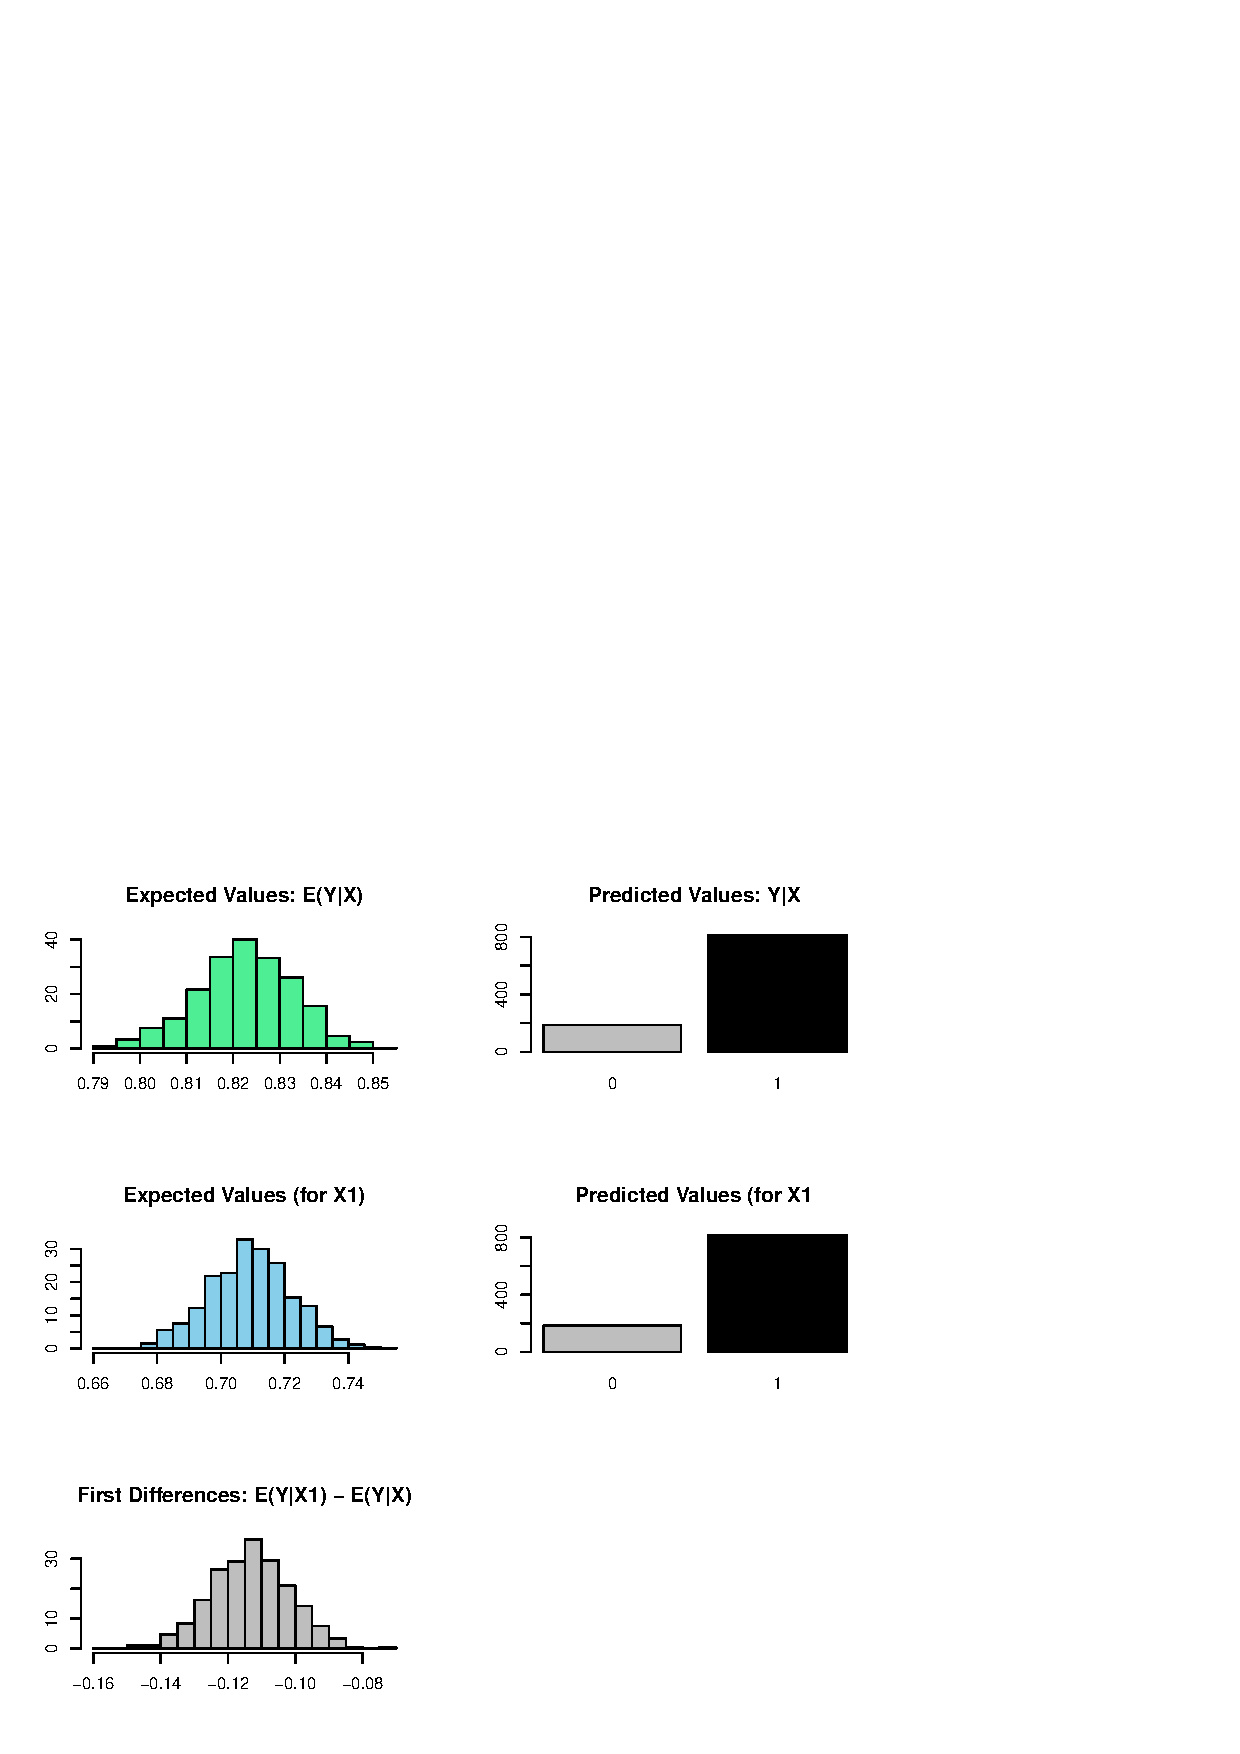
\includegraphics{vigpics/logit-FirstDifferencesPlot}
\end{center} 


\item {Presenting Results: An ROC Plot}  \label{ROC}
  
  One can use an ROC plot to evaluate the fit of alternative model
  specifications.  (Use {\tt demo(roc)} to view this example, or see
  King and Zeng (2002)\nocite{KinZen02}.)  
\begin{Schunk}
\begin{Sinput}
> z.out1 <- zelig(vote ~ race + educate + age, model = "logit", 
+     data = turnout)
> z.out2 <- zelig(vote ~ race + educate, model = "logit", data = turnout)
\end{Sinput}
\end{Schunk}
\begin{center}
\begin{Schunk}
\begin{Sinput}
> rocplot(z.out1$y, z.out2$y, fitted(z.out1), fitted(z.out2))
\end{Sinput}
\end{Schunk}
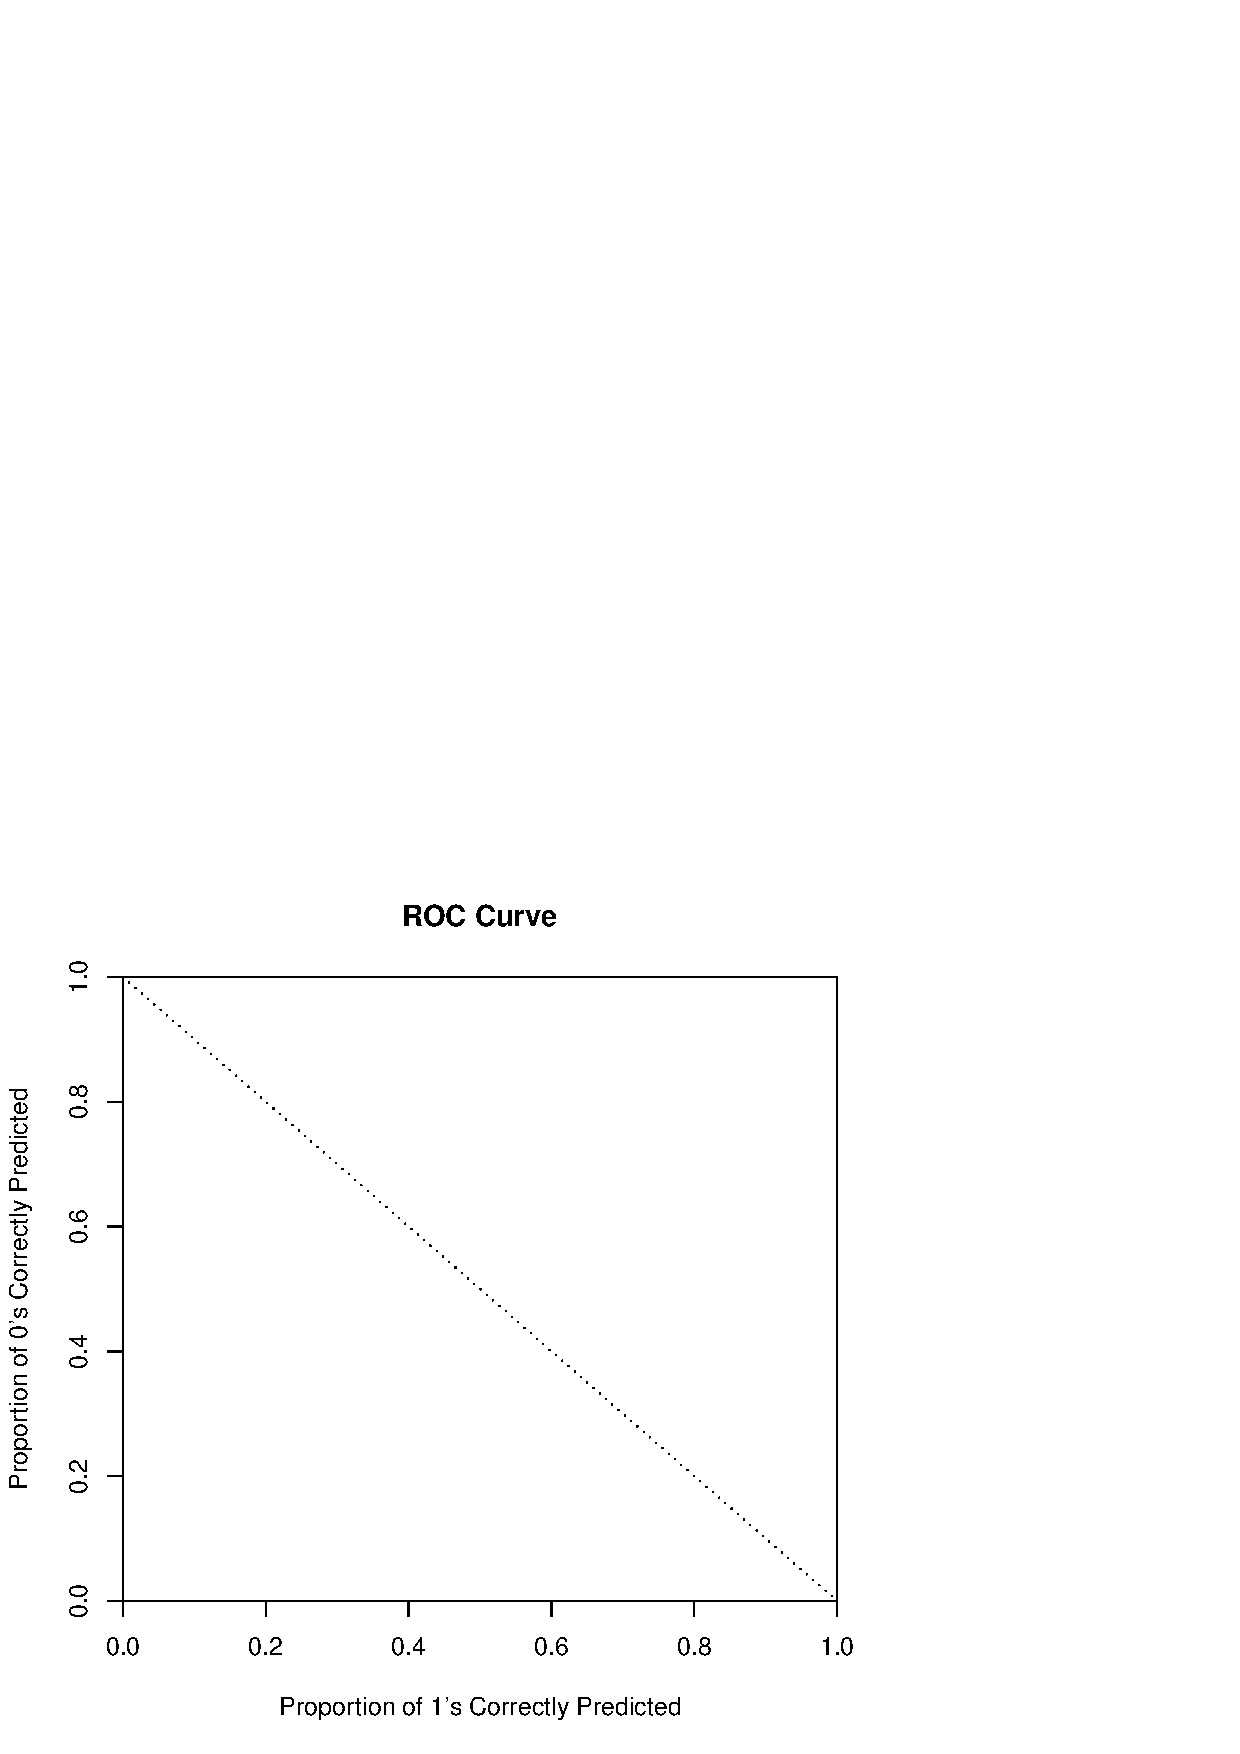
\includegraphics{vigpics/logit-ROCPlot}
\end{center}
\end{enumerate}

\subsubsection{Model}
Let $Y_i$ be the binary dependent variable for observation $i$ which
takes the value of either 0 or 1.
\begin{itemize}

\item The \emph{stochastic component} is given by  
\begin{eqnarray*}
Y_i &\sim& \textrm{Bernoulli}(y_i \mid \pi_i) \\
    &=& \pi_i^{y_i} (1-\pi_i)^{1-y_i}
\end{eqnarray*}
where $\pi_i=\Pr(Y_i=1)$.

\item The \emph{systematic component} is given by: 
\begin{equation*}
\pi_i \; = \; \frac{1}{1 + \exp(-x_i \beta)}.
\end{equation*}
where $x_i$ is the vector of $k$ explanatory variables for observation $i$
and $\beta$ is the vector of coefficients.
\end{itemize}

\subsubsection{Quantities of Interest}
\begin{itemize}
\item The expected values ({\tt qi\$ev}) for the logit model are
  simulations of the predicted probability of a success: $$E(Y) =
  \pi_i= \frac{1}{1 + \exp(-x_i \beta)},$$ given draws of $\beta$ from
  its sampling distribution.

\item The predicted values ({\tt qi\$pr}) are draws from the Binomial
  distribution with mean equal to the simulated expected value $\pi_i$.  

\item The first difference ({\tt qi\$fd}) for the logit model is defined as
\begin{equation*}
\textrm{FD} = \Pr(Y = 1 \mid x_1) - \Pr(Y = 1 \mid x).
\end{equation*}

\item The risk ratio ({\tt qi\$rr}) is defined as
\begin{equation*}
\textrm{RR} = \Pr(Y = 1 \mid x_1) \ / \ \Pr(Y = 1 \mid x).
\end{equation*}

\item In conditional prediction models, the average expected treatment
  effect ({\tt att.ev}) for the treatment group is 
    \begin{equation*} \frac{1}{\sum_{i=1}^n t_i}\sum_{i:t_i=1}^n \left\{ Y_i(t_i=1) -
      E[Y_i(t_i=0)] \right\},
    \end{equation*} 
    where $t_i$ is a binary explanatory variable defining the treatment
    ($t_i=1$) and control ($t_i=0$) groups.  Variation in the
    simulations are due to uncertainty in simulating $E[Y_i(t_i=0)]$,
    the counterfactual expected value of $Y_i$ for observations in the
    treatment group, under the assumption that everything stays the
    same except that the treatment indicator is switched to $t_i=0$.

\item In conditional prediction models, the average predicted treatment
  effect ({\tt att.pr}) for the treatment group is 
    \begin{equation*} \frac{1}{\sum_{i=1}^n t_i}\sum_{i:t_i=1}^n \left\{ Y_i(t_i=1) -
      \widehat{Y_i(t_i=0)}\right\},
    \end{equation*} 
    where $t_i$ is a binary explanatory variable defining the
    treatment ($t_i=1$) and control ($t_i=0$) groups.  Variation in
    the simulations are due to uncertainty in simulating
    $\widehat{Y_i(t_i=0)}$, the counterfactual predicted value of
    $Y_i$ for observations in the treatment group, under the
    assumption that everything stays the same except that the
    treatment indicator is switched to $t_i=0$.
\end{itemize}

\subsubsection{Output Values}

The output of each Zelig command contains useful information which you
may view.  For example, if you run \texttt{z.out <- zelig(y \~\, x,
  model = "logit", data)}, then you may examine the available
information in \texttt{z.out} by using \texttt{names(z.out)},
see the {\tt coefficients} by using {\tt z.out\$coefficients}, and
a default summary of information through \texttt{summary(z.out)}.
Other elements available through the {\tt \$} operator are listed
below.

\begin{itemize}
\item From the {\tt zelig()} output object {\tt z.out}, you may
  extract:
   \begin{itemize}
   \item {\tt coefficients}: parameter estimates for the explanatory
     variables.
   \item {\tt residuals}: the working residuals in the final iteration
     of the IWLS fit.
   \item {\tt fitted.values}: the vector of fitted values for the
     systemic component, $\pi_i$.
   \item {\tt linear.predictors}: the vector of $x_{i}\beta$
   \item {\tt aic}: Akaike's Information Criterion (minus twice the
     maximized log-likelihood plus twice the number of coefficients).
   \item {\tt df.residual}: the residual degrees of freedom.
   \item {\tt df.null}: the residual degrees of freedom for the null
     model.
   \item {\tt data}: the name of the input data frame.  
   \end{itemize}

\item From {\tt summary(z.out)}, you may extract: 
   \begin{itemize}
   \item {\tt coefficients}: the parameter estimates with their
     associated standard errors, $p$-values, and $t$-statistics.
   \item{\tt cov.scaled}: a $k \times k$ matrix of scaled covariances.
   \item{\tt cov.unscaled}: a $k \times k$ matrix of unscaled
     covariances.  
   \end{itemize}

\item From the {\tt sim()} output object {\tt s.out}, you may extract
  quantities of interest arranged as matrices indexed by simulation
  $\times$ {\tt x}-observation (for more than one {\tt x}-observation).
  Available quantities are:

   \begin{itemize}
   \item {\tt qi\$ev}: the simulated expected probabilities for the
     specified values of {\tt x}.
   \item {\tt qi\$pr}: the simulated predicted values for the
     specified values of {\tt x}.
   \item {\tt qi\$fd}: the simulated first difference in the expected
     probabilities for the values specified in {\tt x} and {\tt x1}.
   \item {\tt qi\$rr}: the simulated risk ratio for the expected
     probabilities simulated from {\tt x} and {\tt x1}.
   \item {\tt qi\$att.ev}: the simulated average expected treatment
     effect for the treated from conditional prediction models.  
   \item {\tt qi\$att.pr}: the simulated average predicted treatment
     effect for the treated from conditional prediction models.  
   \end{itemize}
\end{itemize}

\subsection* {How to Cite} 

\input{cites/logit}
\input{citeZelig}


\subsection*{See also}

The logit model is part of the stats package by \citet{VenRip02}.
Advanced users may wish to refer to \texttt{help(glm)} and
\texttt{help(family)}, as well as \cite{McCNel89}. Robust standard
errors are implemented via the sandwich package by \citet{Zeileis04}.
Sample data are from \cite{KinTomWit00}.

\bibliographystyle{asa}
\bibliography{gk,gkpubs}
 \end{document}

%%% Local Variables: 
%%% mode: latex
%%% TeX-master: t
%%% End: 










To cite Zelig as a whole, please reference these two sources:
\begin{verse}
  Kosuke Imai, Gary King, and Olivia Lau. 2007. ``Zelig: Everyone's
  Statistical Software,'' \url{http://GKing.harvard.edu/zelig}.
\end{verse}
\begin{verse}
Imai, Kosuke, Gary King, and Olivia Lau. (2008). ``Toward A Common Framework for Statistical Analysis and Development.'' Journal of Computational and Graphical Statistics, Vol. 17, No. 4 (December), pp. 892-913. 
\end{verse}



\subsection*{See also}

The logit model is part of the stats package by \citet{VenRip02}.
Advanced users may wish to refer to \texttt{help(glm)} and
\texttt{help(family)}, as well as \cite{McCNel89}. Robust standard
errors are implemented via the sandwich package by \citet{Zeileis04}.
Sample data are from \cite{KinTomWit00}.

\bibliographystyle{asa}
\bibliography{gk,gkpubs}
 \end{document}

%%% Local Variables: 
%%% mode: latex
%%% TeX-master: t
%%% End: 










To cite Zelig as a whole, please reference these two sources:
\begin{verse}
  Kosuke Imai, Gary King, and Olivia Lau. 2007. ``Zelig: Everyone's
  Statistical Software,'' \url{http://GKing.harvard.edu/zelig}.
\end{verse}
\begin{verse}
Imai, Kosuke, Gary King, and Olivia Lau. (2008). ``Toward A Common Framework for Statistical Analysis and Development.'' Journal of Computational and Graphical Statistics, Vol. 17, No. 4 (December), pp. 892-913. 
\end{verse}



\subsection*{See also}

The logit model is part of the stats package by \citet{VenRip02}.
Advanced users may wish to refer to \texttt{help(glm)} and
\texttt{help(family)}, as well as \cite{McCNel89}. Robust standard
errors are implemented via the sandwich package by \citet{Zeileis04}.
Sample data are from \cite{KinTomWit00}.

\bibliographystyle{asa}
\bibliography{gk,gkpubs}
 \end{document}

%%% Local Variables: 
%%% mode: latex
%%% TeX-master: t
%%% End: 










\documentclass{article}

\title{
  ls: Least Squares Regression for Continuous
  Dependent Variables
}
\author{Matt Owen, Olivia Lau, Kosuke Imai, and Gary King}




\usepackage{bibentry}
\usepackage{graphicx}
\usepackage{natbib}
\usepackage{amsmath}
\usepackage{url}
\usepackage{Zelig}
\usepackage{Sweave}

%\VignetteIndexEntry{Least Squares Regression for Continuous Dependent Variables}
%\VignetteDepends{Zelig, stats}
%\VignetteKeyWords{model,least squares,continuous, regression}
%\VignettePackage{Zelig}

\begin{document}

\nobibliography*



\section{{\tt ls}: Least Squares Regression for Continuous
Dependent Variables}
\label{ls}

Use least squares regression analysis to estimate the best linear
predictor for the specified dependent variables.

\subsubsection{Syntax}

\begin{verbatim}
> z.out <- zelig(Y ~ X1 + X2, model = "ls", data = mydata)
> x.out <- setx(z.out)
> s.out <- sim(z.out, x = x.out)
\end{verbatim}

\subsubsection{Additional Inputs}  

In addition to the standard inputs, {\tt zelig()} takes the following
additional options for least squares regression:  
\begin{itemize}
\item {\tt robust}: defaults to {\tt FALSE}.  If {\tt TRUE} is
selected, {\tt zelig()} computes robust standard errors based on
sandwich estimators (see \cite{Zeileis04}, \cite{Huber81}, and
\cite{White80}).  The default type of robust standard error is
heteroskedastic consistent (HC), \emph{not} heteroskedastic and
autocorrelation consistent (HAC).  

In addition, {\tt robust} may be a list with the following options:  
\begin{itemize}
\item {\tt method}:  choose from 
\begin{itemize}
\item {\tt "vcovHC"}: (the default if {\tt robust = TRUE}), HC standard errors.
\item {\tt "vcovHAC"}: HAC standard errors without weights.  
\item {\tt "kernHAC"}: HAC standard errors using the weights given in
\cite{Andrews91}.   
\item {\tt "weave"}: HAC standard errors using the weights given in
\cite{LumHea99}.
\end{itemize} 
\item {\tt order.by}: only applies to the HAC methods above.  Defaults to
{\tt NULL} (the observations are chronologically ordered as in the
original data).  Optionally, you may specify a time index (either as
{\tt order.by = z}, where {\tt z} exists outside the data frame; or
as {\tt order.by = \~{}z}, where {\tt z} is a variable in the data
frame).  The observations are chronologically ordered by the size of
{\tt z}.
\item {\tt \dots}:  additional options passed to the functions
specified in {\tt method}.  See the {\tt sandwich} library and
\cite{Zeileis04} for more options.   
\end{itemize}
\end{itemize}

\subsubsection{Examples}\begin{enumerate}
\item Basic Example with First Differences

Attach sample data:
\begin{Schunk}
\begin{Sinput}
>  data(macro)
\end{Sinput}
\end{Schunk}
Estimate model:
\begin{Schunk}
\begin{Sinput}
>  z.out1 <- zelig(unem ~ gdp + capmob + trade, model = "ls", data = macro)
\end{Sinput}
\end{Schunk}
Summarize regression coefficients:
\begin{Schunk}
\begin{Sinput}
>  summary(z.out1)
\end{Sinput}
\end{Schunk}
Set explanatory variables to their default (mean/mode) values, with
high (80th percentile) and low (20th percentile) values for the trade variable:
\begin{Schunk}
\begin{Sinput}
>  x.high <- setx(z.out1, trade = quantile(macro$trade, 0.8))
\documentclass{article}

\usepackage{Zelig}



\usepackage{Sweave}
\begin{document}
\nobibliography*



\section{{\tt negbinom}: Negative Binomial Regression for Event
Count Dependent Variables}\label{negbinom}

Use the negative binomial regression if you have a count of events for
each observation of your dependent variable.  The negative binomial
model is frequently used to estimate over-dispersed event count
models.

\subsubsection{Syntax}

\begin{verbatim}
> z.out <- zelig(Y ~ X1 + X2, model = "negbinom", data = mydata)
> x.out <- setx(z.out)
> s.out <- sim(z.out, x = x.out)
\end{verbatim}

\subsubsection{Additional Inputs} 

In addition to the standard inputs, {\tt zelig()} takes the following
additional options for negative binomial regression:  
\begin{itemize}
\item {\tt robust}: defaults to {\tt FALSE}.  If {\tt TRUE} is
selected, {\tt zelig()} computes robust standard errors via the {\tt
sandwich} package (see \cite{Zeileis04}).  The default type of robust
standard error is heteroskedastic and autocorrelation consistent (HAC),
and assumes that observations are ordered by time index.

In addition, {\tt robust} may be a list with the following options:  
\begin{itemize}
\item {\tt method}:  Choose from 
\begin{itemize}
\item {\tt "vcovHAC"}: (default if {\tt robust = TRUE}) HAC standard
errors. 
\item {\tt "kernHAC"}: HAC standard errors using the
weights given in \cite{Andrews91}. 
\item {\tt "weave"}: HAC standard errors using the
weights given in \cite{LumHea99}.  
\end{itemize}  
\item {\tt order.by}: defaults to {\tt NULL} (the observations are
chronologically ordered as in the original data).  Optionally, you may
specify a vector of weights (either as {\tt order.by = z}, where {\tt
z} exists outside the data frame; or as {\tt order.by = \~{}z}, where
{\tt z} is a variable in the data frame).  The observations are
chronologically ordered by the size of {\tt z}.
\item {\tt \dots}:  additional options passed to the functions 
specified in {\tt method}.   See the {\tt sandwich} library and
\cite{Zeileis04} for more options.   
\end{itemize}
\end{itemize}

\subsubsection{Example}

Load sample data:  
\begin{Schunk}
\begin{Sinput}
> data(sanction)
\end{Sinput}
\end{Schunk}
Estimate the model:  
\begin{Schunk}
\begin{Sinput}
> z.out <- zelig(num ~ target + coop, model = "negbinom", data = sanction)
\end{Sinput}
\end{Schunk}
\begin{Schunk}
\begin{Sinput}
> summary(z.out)
\end{Sinput}
\end{Schunk}
Set values for the explanatory variables to their default mean values:  
\begin{Schunk}
\begin{Sinput}
> x.out <- setx(z.out)
\end{Sinput}
\end{Schunk}
Simulate fitted values:  
\begin{Schunk}
\begin{Sinput}
> s.out <- sim(z.out, x = x.out)
\end{Sinput}
\end{Schunk}
\begin{Schunk}
\begin{Sinput}
> summary(s.out)
\end{Sinput}
\end{Schunk}
\begin{center}
\begin{Schunk}
\begin{Sinput}
> plot(s.out)
\end{Sinput}
\end{Schunk}
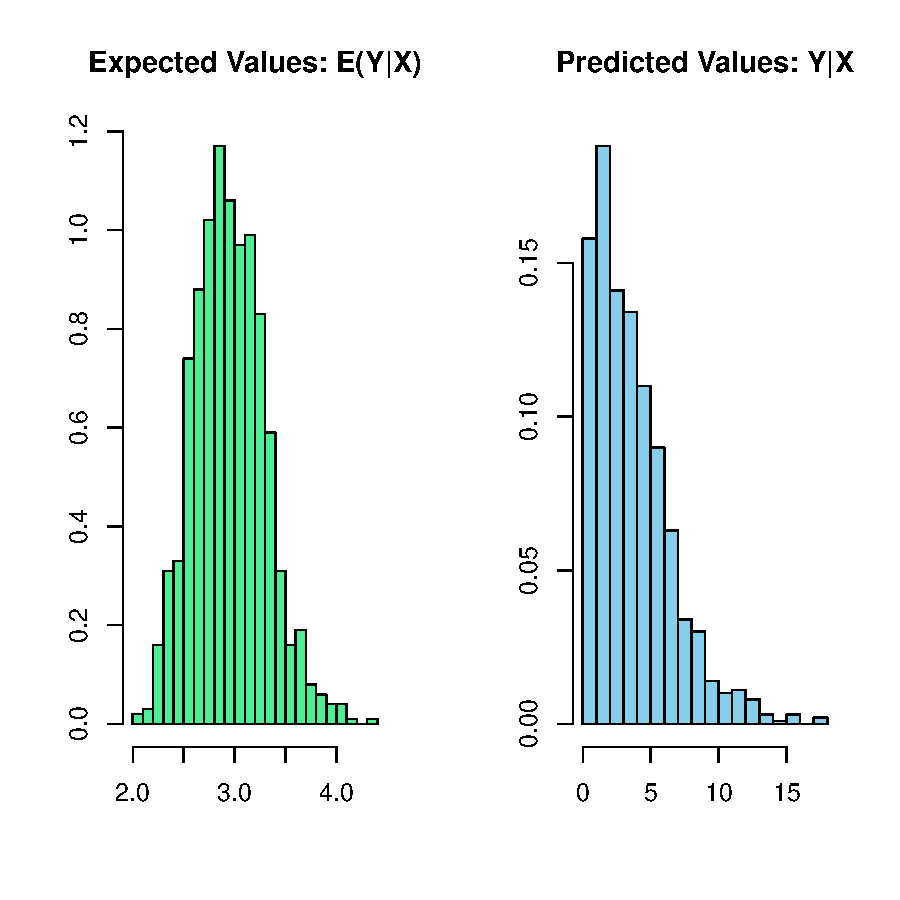
\includegraphics{vigpics/negbin-Example1Plot}
\end{center}
\subsubsection{Model}
Let $Y_i$ be the number of independent events that occur during a
fixed time period. This variable can take any non-negative integer value.

\begin{itemize}
\item The negative binomial distribution is derived by letting the
  mean of the Poisson distribution vary according to a fixed
  parameter $\zeta$ given by the Gamma distribution. The
  \emph{stochastic component} is given by
   \begin{eqnarray*}
     Y_i \mid \zeta_i & \sim & \textrm{Poisson}(\zeta_i \mu_i),\\
     \zeta_i & \sim & \frac{1}{\theta}\textrm{Gamma}(\theta).
   \end{eqnarray*}
   The marginal distribution of $Y_i$ is then the negative binomial
   with mean $\mu_i$ and variance $\mu_i + \mu_i^2/\theta$:
   \begin{eqnarray*}
   Y_i & \sim & \textrm{NegBinom}(\mu_i, \theta), \\
       & = & \frac{\Gamma (\theta + y_i)}{y! \, \Gamma(\theta)} 
             \frac{\mu_i^{y_i} \, \theta^{\theta}}{(\mu_i + \theta)^{\theta + y_i}},
   \end{eqnarray*}
   where $\theta$ is the systematic parameter of the Gamma
   distribution modeling $\zeta_i$.  

 \item The \emph{systematic component} is given by
   \begin{equation*}
     \mu_i = \exp(x_i \beta)
   \end{equation*}
   where $x_i$ is the vector of $k$ explanatory variables and $\beta$ is
   the vector of coefficients.
 \end{itemize}

\subsubsection{Quantities of Interest}
\begin{itemize}
\item The expected values ({\tt qi\$ev}) are simulations of the mean
  of the stochastic component.  Thus, $$E(Y) = \mu_i = \exp(x_i
  \beta),$$ given simulations of $\beta$.  
  
\item The predicted value ({\tt qi\$pr}) drawn from the distribution
  defined by the set of parameters $(\mu_i, \theta)$.

\item The first difference ({\tt qi\$fd}) is
\begin{equation*}
\textrm{FD} \; = \; E(Y | x_1) - E(Y \mid x)
\end{equation*}
\item In conditional prediction models, the average expected treatment
  effect ({\tt att.ev}) for the treatment group is 
    \begin{equation*} \frac{1}{\sum_{i=1}^n t_i}\sum_{i:t_i=1}^n \left\{ Y_i(t_i=1) -
      E[Y_i(t_i=0)] \right\},
    \end{equation*} 
    where $t_i$ is a binary explanatory variable defining the treatment
    ($t_i=1$) and control ($t_i=0$) groups.  Variation in the
    simulations are due to uncertainty in simulating $E[Y_i(t_i=0)]$,
    the counterfactual expected value of $Y_i$ for observations in the
    treatment group, under the assumption that everything stays the
    same except that the treatment indicator is switched to $t_i=0$.

\item In conditional prediction models, the average predicted treatment
  effect ({\tt att.pr}) for the treatment group is 
    \begin{equation*} \frac{1}{\sum_{i=1}^n t_i}\sum_{i:t_i=1}^n \left\{ Y_i(t_i=1) -
      \widehat{Y_i(t_i=0)} \right\},
    \end{equation*} 
    where $t_i$ is a binary explanatory variable defining the
    treatment ($t_i=1$) and control ($t_i=0$) groups.  Variation in
    the simulations are due to uncertainty in simulating
    $\widehat{Y_i(t_i=0)}$, the counterfactual predicted value of
    $Y_i$ for observations in the treatment group, under the
    assumption that everything stays the same except that the
    treatment indicator is switched to $t_i=0$.
\end{itemize}

\subsubsection{Output Values}

The output of each Zelig command contains useful information which you
may view.  For example, if you run \texttt{z.out <- zelig(y \~\,
  x, model = "negbinom", data)}, then you may examine the available
information in \texttt{z.out} by using \texttt{names(z.out)},
see the {\tt coefficients} by using {\tt z.out\$coefficients}, and
a default summary of information through \texttt{summary(z.out)}.
Other elements available through the {\tt \$} operator are listed
below.

\begin{itemize}
\item From the {\tt zelig()} output object {\tt z.out}, you may extract:
   \begin{itemize}
   \item {\tt coefficients}: parameter estimates for the explanatory
     variables.
   \item {\tt theta}: the maximum likelihood estimate for the
     stochastic parameter $\theta$.  
   \item {\tt SE.theta}: the standard error for {\tt theta}.  
   \item {\tt residuals}: the working residuals in the final iteration
     of the IWLS fit.
   \item {\tt fitted.values}: a vector of the fitted values for the systemic
     component $\lambda$.  
   \item {\tt linear.predictors}: a vector of $x_{i} \beta$.  
   \item {\tt aic}: Akaike's Information Criterion (minus twice the
     maximized log-likelihood plus twice the number of coefficients).
   \item {\tt df.residual}: the residual degrees of freedom.
   \item {\tt df.null}: the residual degrees of freedom for the null
     model.
   \item {\tt zelig.data}: the input data frame if {\tt save.data = TRUE}.  
   \end{itemize}

\item From {\tt summary(z.out)}, you may extract: 
   \begin{itemize}
   \item {\tt coefficients}: the parameter estimates with their
     associated standard errors, $p$-values, and $t$-statistics.
   \item{\tt cov.scaled}: a $k \times k$ matrix of scaled covariances.
   \item{\tt cov.unscaled}: a $k \times k$ matrix of unscaled
     covariances.  
   \end{itemize}

\item From the {\tt sim()} output object {\tt s.out}, you may extract
  quantities of interest arranged as matrices indexed by simulation
  $\times$ {\tt x}-observation (for more than one {\tt x}-observation).
  Available quantities are:

   \begin{itemize}
   \item {\tt qi\$ev}: the simulated expected values given the specified
     values of {\tt x}.
   \item {\tt qi\$pr}: the simulated predicted values drawn from the
     distribution defined by $(\mu_i, \theta)$.  
   \item {\tt qi\$fd}: the simulated first differences in the
     simulated expected values given the specified values of {\tt x}
     and {\tt x1}.
   \item {\tt qi\$att.ev}: the simulated average expected treatment
     effect for the treated from conditional prediction models.  
   \item {\tt qi\$att.pr}: the simulated average predicted treatment
     effect for the treated from conditional prediction models.  
   \end{itemize}
\end{itemize}

\subsection* {How to Cite} 

How to cite this model in Zelig:
\begin{verse}
  Kosuke Imai, Gary King, and Olivia Lau. 2010. "negbinom" in Kosuke Imai, Gary King, and Olivia Lau, "Zelig: Everyone's Statistical Software,"http://gking.harvard.edu/zelig
\end{verse}

\CiteZelig

\subsection* {See also}
The negative binomial model is part of the MASS package by William N. Venable and Brian D. Ripley \citep{VenRip02}. Advanced users may wish to refer to \texttt{help(glm.nb)} as well as \cite{McCNel89}. Robust standard errors are implemented via sandwich package by Achim Zeileis \citep{Zeileis04}.Sample data are from \cite{Martin92}.

\bibliographystyle{asa}
\bibliography{gk,gkpubs}
 \end{document}

%%% Local Variables: 
%%% mode: latex
%%% TeX-master: t
%%% End: 






\documentclass{article}

\usepackage{Zelig}



\usepackage{Sweave}
\begin{document}
\nobibliography*

\section{{\tt normal}: Normal Regression for Continuous Dependent Variables}
\label{normal}

The Normal regression model is a close variant of the more standard
least squares regression model (see \Sref{ls}). Both models specify a
continuous dependent variable as a linear function of a set of
explanatory variables.  The Normal model reports maximum likelihood
(rather than least squares) estimates.  The two models differ only in
their estimate for the stochastic parameter $\sigma$.

\subsubsection{Syntax}

\begin{verbatim}
> z.out <- zelig(Y ~ X1 + X2, model = "normal", data = mydata)
> x.out <- setx(z.out)
> s.out <- sim(z.out, x = x.out)
\end{verbatim}

\subsubsection{Additional Inputs} 

In addition to the standard inputs, {\tt zelig()} takes the following
additional options for normal regression:  
\begin{itemize}
\item {\tt robust}: defaults to {\tt FALSE}.  If {\tt TRUE} is
selected, {\tt zelig()} computes robust standard errors via the {\tt
sandwich} package (see \cite{Zeileis04}).  The default type of robust
standard error is heteroskedastic and autocorrelation consistent (HAC),
and assumes that observations are ordered by time index.

In addition, {\tt robust} may be a list with the following options:  
\begin{itemize}
\item {\tt method}:  Choose from 
\begin{itemize}
\item {\tt "vcovHAC"}: (default if {\tt robust = TRUE}) HAC standard
errors. 
\item {\tt "kernHAC"}: HAC standard errors using the
weights given in \cite{Andrews91}. 
\item {\tt "weave"}: HAC standard errors using the
weights given in \cite{LumHea99}.  
\end{itemize}  
\item {\tt order.by}: defaults to {\tt NULL} (the observations are
chronologically ordered as in the original data).  Optionally, you may
specify a vector of weights (either as {\tt order.by = z}, where {\tt
z} exists outside the data frame; or as {\tt order.by = \~{}z}, where
{\tt z} is a variable in the data frame).  The observations are
chronologically ordered by the size of {\tt z}.
\item {\tt \dots}:  additional options passed to the functions 
specified in {\tt method}.   See the {\tt sandwich} library and
\cite{Zeileis04} for more options.   
\end{itemize}
\end{itemize}

\subsubsection{Examples}

\begin{enumerate}
\item Basic Example with First Differences

Attach sample data: 
\begin{Schunk}
\begin{Sinput}
> data(macro)
\end{Sinput}
\end{Schunk}
Estimate model:  
\begin{Schunk}
\begin{Sinput}
> z.out1 <- zelig(unem ~ gdp + capmob + trade, model = "normal", 
+     data = macro)
\end{Sinput}
\end{Schunk}
Summarize of regression coefficients:  
\begin{Schunk}
\begin{Sinput}
> summary(z.out1)
\end{Sinput}
\end{Schunk}
Set explanatory variables to their default (mean/mode) values, with
high (80th percentile) and low (20th percentile) values for trade: 
\begin{Schunk}
\begin{Sinput}
> x.high <- setx(z.out1, trade = quantile(macro$trade, 0.8))
> x.low <- setx(z.out1, trade = quantile(macro$trade, 0.2))
\end{Sinput}
\end{Schunk}
Generate first differences for the effect of high versus low trade on
GDP: 
\begin{Schunk}
\begin{Sinput}
> s.out1 <- sim(z.out1, x = x.high, x1 = x.low)
\end{Sinput}
\end{Schunk}
\begin{Schunk}
\begin{Sinput}
> summary(s.out1)
\end{Sinput}
\end{Schunk}
%plot does not work 
A visual summary of quantities of interest:  
\begin{center}
\begin{Schunk}
\begin{Sinput}
> plot(s.out1)
\end{Sinput}
\end{Schunk}
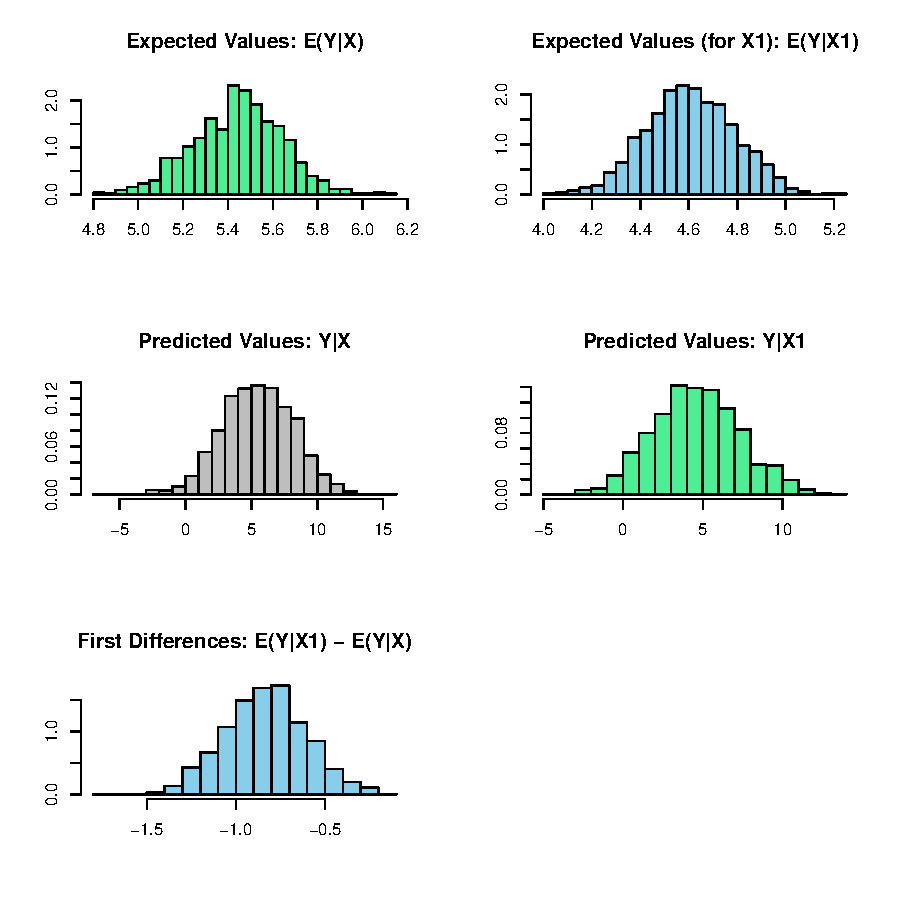
\includegraphics{vigpics/normal-ExamplesPlot}
\end{center}

\item Using Dummy Variables
%the code in this section does not work well but there is no demo for this part either
 
Estimate a model with a dummy variable for each year and country (see
\ref{factors} for help with dummy variables).  Note that you do not
need to create dummy variables, as the program will automatically
parse the unique values in the selected variables into dummy
variables.    
\begin{Schunk}
\begin{Sinput}
> z.out2 <- zelig(unem ~ gdp + trade + capmob + as.factor(year) + 
+     as.factor(country), model = "normal", data = macro)
\end{Sinput}
\end{Schunk}
Set values for the explanatory variables, using the default mean/mode
variables, with country set to the United States and Japan,
respectively: 
Simulate quantities of interest:  
%plot does not work 
\begin{center}
\end{center}
\end{enumerate}

\subsubsection{Model}
Let $Y_i$ be the continuous dependent variable for observation $i$.
\begin{itemize}
\item The \emph{stochastic component} is described by a univariate normal
  model with a vector of means $\mu_i$ and scalar variance $\sigma^2$:
  \begin{equation*}
    Y_i \; \sim \; \textrm{Normal}(\mu_i, \sigma^2). 
  \end{equation*}

\item The \emph{systematic component} is 
  \begin{equation*}
    \mu_i \;= \; x_i \beta,
  \end{equation*}
  where $x_i$ is the vector of $k$ explanatory variables and $\beta$ is
  the vector of coefficients.
\end{itemize}


\subsubsection{Quantities of Interest}

\begin{itemize}
\item The expected value ({\tt qi\$ev}) is the mean of simulations
  from the the stochastic component, $$E(Y) = \mu_i = x_i \beta,$$
  given a draw of $\beta$ from its posterior.  

\item The predicted value ({\tt qi\$pr}) is drawn from the distribution
  defined by the set of parameters $(\mu_i, \sigma)$.  

\item The first difference ({\tt qi\$fd}) is:
\begin{equation*}
\textrm{FD}\; = \;E(Y \mid x_1) -  E(Y \mid x)
\end{equation*}

\item In conditional prediction models, the average expected treatment
  effect ({\tt att.ev}) for the treatment group is 
    \begin{equation*} \frac{1}{\sum_{i=1}^n t_i}\sum_{i:t_i=1}^n \left\{ Y_i(t_i=1) -
      E[Y_i(t_i=0)] \right\},
    \end{equation*} 
    where $t_i$ is a binary explanatory variable defining the treatment
    ($t_i=1$) and control ($t_i=0$) groups.  Variation in the
    simulations are due to uncertainty in simulating $E[Y_i(t_i=0)]$,
    the counterfactual expected value of $Y_i$ for observations in the
    treatment group, under the assumption that everything stays the
    same except that the treatment indicator is switched to $t_i=0$.

\item In conditional prediction models, the average predicted treatment
  effect ({\tt att.pr}) for the treatment group is 
    \begin{equation*} \frac{1}{\sum_{i=1}^n t_i}\sum_{i:t_i=1}^n \left\{ Y_i(t_i=1) -
      \widehat{Y_i(t_i=0)} \right\},
    \end{equation*} 
    where $t_i$ is a binary explanatory variable defining the
    treatment ($t_i=1$) and control ($t_i=0$) groups.  Variation in
    the simulations are due to uncertainty in simulating
    $\widehat{Y_i(t_i=0)}$, the counterfactual predicted value of
    $Y_i$ for observations in the treatment group, under the
    assumption that everything stays the same except that the
    treatment indicator is switched to $t_i=0$.

\end{itemize}

\subsubsection{Output Values}

The output of each Zelig command contains useful information which you
may view.  For example, if you run \texttt{z.out <- zelig(y \~\,
  x, model = "normal", data)}, then you may examine the available
information in \texttt{z.out} by using \texttt{names(z.out)},
see the {\tt coefficients} by using {\tt z.out\$coefficients}, and
a default summary of information through \texttt{summary(z.out)}.
Other elements available through the {\tt \$} operator are listed
below.

\begin{itemize}
\item From the {\tt zelig()} output object {\tt z.out}, you may extract:
   \begin{itemize}
   \item {\tt coefficients}: parameter estimates for the explanatory
     variables.
   \item {\tt residuals}: the working residuals in the final iteration
     of the IWLS fit.
   \item {\tt fitted.values}: fitted values.  For the normal model,
     these are identical to the {\tt linear predictors}.
   \item {\tt linear.predictors}: fitted values.  For the normal
     model, these are identical to {\tt fitted.values}.
   \item {\tt aic}: Akaike's Information Criterion (minus twice the
     maximized log-likelihood plus twice the number of coefficients).
   \item {\tt df.residual}: the residual degrees of freedom.
   \item {\tt df.null}: the residual degrees of freedom for the null
     model.
   \item {\tt zelig.data}: the input data frame if {\tt save.data = TRUE}.  
   \end{itemize}

\item From {\tt summary(z.out)}, you may extract: 
   \begin{itemize}
   \item {\tt coefficients}: the parameter estimates with their
     associated standard errors, $p$-values, and $t$-statistics.
   \item{\tt cov.scaled}: a $k \times k$ matrix of scaled covariances.
   \item{\tt cov.unscaled}: a $k \times k$ matrix of unscaled
     covariances.  
   \end{itemize}

\item From the {\tt sim()} output object {\tt s.out}, you may extract
  quantities of interest arranged as matrices indexed by simulation
  $\times$ {\tt x}-observation (for more than one {\tt x}-observation).
  Available quantities are:

   \begin{itemize}
   \item {\tt qi\$ev}: the simulated expected values for the specified
     values of {\tt x}.
   \item {\tt qi\$pr}: the simulated predicted values drawn from the
     distribution defined by $(\mu_i, \sigma)$.
   \item {\tt qi\$fd}: the simulated first difference in the simulated
     expected values for the values specified in {\tt x} and {\tt x1}.
   \item {\tt qi\$att.ev}: the simulated average expected treatment
     effect for the treated from conditional prediction models.  
   \item {\tt qi\$att.pr}: the simulated average predicted treatment
     effect for the treated from conditional prediction models.  
   \end{itemize}
\end{itemize}

\subsection* {How to Cite} 

How to cite this model in Zelig:
\begin{verse}
  Kosuke Imai, Gary King, and Olivia Lau. 2008. "normal: Normal Regression for Continuous Dependent Variables" in Kosuke Imai, Gary King, and Olivia Lau, "Zelig: Everyone's Statistical Software,"http://gking.harvard.edu/zelig
\end{verse}

\CiteZelig

\subsection* {See also}

The normal model is part of the stats package by \citet{VenRip02}.
Advanced users may wish to refer to \texttt{help(glm)} and
\texttt{help(family)}, as well as \cite{McCNel89}. Robust standard
errors are implemented via the sandwich package by \citet{Zeileis04}.
Sample data are from \cite{KinTomWit00}.

\bibliographystyle{asa}
\bibliography{gk,gkpubs}
 \end{document}


%%% Local Variables: 
%%% mode: latex
%%% TeX-master: t
%%% End: 














\documentclass[oneside,letterpaper,12pt]{book}
\usepackage{Rd}
%\usepackage{Sweave}
%\usepackage{/usr/lib64/R/share/texmf/Sweave}
%\usepackage{/usr/share/R/texmf/Sweave}
\usepackage{bibentry}
\usepackage{upquote}
\usepackage{graphicx}
\usepackage{natbib}
\usepackage[reqno]{amsmath}
\usepackage{amssymb}
\usepackage{amsfonts}
\usepackage{amsmath}
\usepackage{verbatim}
\usepackage{epsf}
\usepackage{url}
\usepackage{html}
\usepackage{dcolumn}
\usepackage{multirow}
\usepackage{fullpage}
\usepackage{lscape}
\usepackage[all]{xy}

\usepackage{csquotes}
% \usepackage[pdftex, bookmarksopen=true,bookmarksnumbered=true,
%   linkcolor=webred]{hyperref}
\bibpunct{(}{)}{;}{a}{}{,}
\newcolumntype{.}{D{.}{.}{-1}}
\newcolumntype{d}[1]{D{.}{.}{#1}}
\htmladdtonavigation{
  \htmladdnormallink{%
    \htmladdimg{http://gking.harvard.edu/pics/home.gif}}
  {http://gking.harvard.edu/}}
\newcommand{\MatchIt}{{\sc MatchIt}}
\newcommand{\hlink}{\htmladdnormallink}
\newcommand{\Sref}[1]{Section~\ref{#1}}
\newcommand{\fullrvers}{2.5.1}
\newcommand{\rvers}{2.5}
\newcommand{\rwvers}{R-2.5.1}
%\renewcommand{\bibentry}{\citealt}

\bodytext{ BACKGROUND="http://gking.harvard.edu/pics/temple.jpg"}
\setcounter{tocdepth}{2}

%\VignetteIndexEntry{Poisson Regression for Event Count Dependent Variables}
%\VignetteDepends{Zelig, stats}
%\VignetteKeyWords{model, poisson,regression, count}
%\VignettePackage{Zelig}
\usepackage{Sweave}
\begin{document}
\nobibliography*


\section{{\tt poisson}: Poisson Regression for Event Count
Dependent Variables}\label{poisson}

Use the Poisson regression model if the observations of your dependent
variable represents the number of independent events that occur during
a fixed period of time (see the negative binomial model, \Sref{negbin},
for over-dispersed event counts.)  For a Bayesian implementation of
this model, see \Sref{poisson.bayes}.  

\subsubsection{Syntax}

\begin{verbatim}
> z.out <- zelig(Y ~ X1 + X2, model = "poisson", data = mydata)
> x.out <- setx(z.out)
> s.out <- sim(z.out, x = x.out)
\end{verbatim}

\subsubsection{Additional Inputs} 

In addition to the standard inputs, {\tt zelig()} takes the following
additional options for poisson regression:  
\begin{itemize}
\item {\tt robust}: defaults to {\tt FALSE}.  If {\tt TRUE} is
selected, {\tt zelig()} computes robust standard errors via the {\tt
sandwich} package (see \cite{Zeileis04}).  The default type of robust
standard error is heteroskedastic and autocorrelation consistent (HAC),
and assumes that observations are ordered by time index.

In addition, {\tt robust} may be a list with the following options:  
\begin{itemize}
\item {\tt method}:  Choose from 
\begin{itemize}
\item {\tt "vcovHAC"}: (default if {\tt robust = TRUE}) HAC standard
errors. 
\item {\tt "kernHAC"}: HAC standard errors using the
weights given in \cite{Andrews91}. 
\item {\tt "weave"}: HAC standard errors using the
weights given in \cite{LumHea99}.  
\end{itemize}  
\item {\tt order.by}: defaults to {\tt NULL} (the observations are
chronologically ordered as in the original data).  Optionally, you may
specify a vector of weights (either as {\tt order.by = z}, where {\tt
z} exists outside the data frame; or as {\tt order.by = \~{}z}, where
{\tt z} is a variable in the data frame).  The observations are
chronologically ordered by the size of {\tt z}.
\item {\tt \dots}:  additional options passed to the functions 
specified in {\tt method}.   See the {\tt sandwich} library and
\cite{Zeileis04} for more options.   
\end{itemize}
\end{itemize}

\subsubsection{Example}

Load sample data:  
\begin{Schunk}
\begin{Sinput}
> data(sanction)
\end{Sinput}
\end{Schunk}
Estimate Poisson model:  
\begin{Schunk}
\begin{Sinput}
> z.out <- zelig(num ~ target + coop, model = "poisson", data = sanction)
\end{Sinput}
\end{Schunk}
\begin{Schunk}
\begin{Sinput}
> summary(z.out)
\end{Sinput}
\end{Schunk}
Set values for the explanatory variables to their default mean values:  
\begin{Schunk}
\begin{Sinput}
> x.out <- setx(z.out)
\end{Sinput}
\end{Schunk}
Simulate fitted values:  
\begin{Schunk}
\begin{Sinput}
> s.out <- sim(z.out, x = x.out)
\end{Sinput}
\end{Schunk}
\begin{Schunk}
\begin{Sinput}
> summary(s.out)
\end{Sinput}
\end{Schunk}
\begin{center}
\begin{Schunk}
\begin{Sinput}
> plot(s.out)
\end{Sinput}
\end{Schunk}
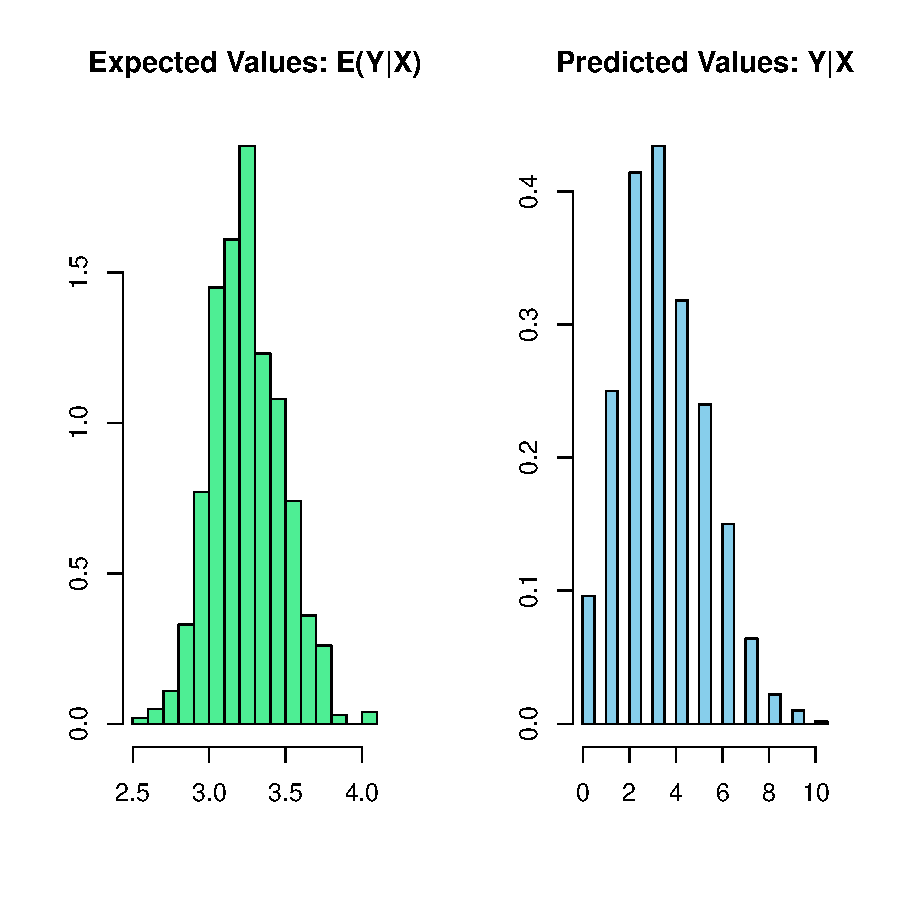
\includegraphics{vigpics/poisson-ExamplePlot}
\end{center}

\subsubsection{Model}
Let $Y_i$ be the number of independent events that occur during a
fixed time period. This variable can take any non-negative integer.

\begin{itemize}
\item The Poisson distribution has \emph{stochastic component}
  \begin{equation*}
    Y_i \; \sim \; \textrm{Poisson}(\lambda_i),
  \end{equation*}
  where $\lambda_i$ is the mean and variance parameter.
  
\item The \emph{systematic component} is 
  \begin{equation*}
    \lambda_i \; = \; \exp(x_i \beta),
  \end{equation*}
  where $x_i$ is the vector of explanatory variables, and $\beta$ is
  the vector of coefficients.
\end{itemize}

\subsubsection{Quantities of Interest}

\begin{itemize}
  
\item The expected value ({\tt qi\$ev}) is the mean of simulations
  from the stochastic component, $$E(Y) = \lambda_i =  \exp(x_i
  \beta),$$ given draws of $\beta$ from its sampling distribution.  
  
\item The predicted value ({\tt qi\$pr}) is a random draw from the
  poisson distribution defined by mean $\lambda_i$.

\item The first difference in the expected values ({\tt qi\$fd}) is given by:
\begin{equation*}
\textrm{FD} \; = \; E(Y | x_1) - E(Y \mid x)
\end{equation*}
\item In conditional prediction models, the average expected treatment
  effect ({\tt att.ev}) for the treatment group is 
    \begin{equation*} \frac{1}{\sum_{i=1}^n t_i}\sum_{i:t_i=1}^n \left\{ Y_i(t_i=1) -
      E[Y_i(t_i=0)] \right\},
    \end{equation*} 
    where $t_i$ is a binary explanatory variable defining the treatment
    ($t_i=1$) and control ($t_i=0$) groups.  Variation in the
    simulations are due to uncertainty in simulating $E[Y_i(t_i=0)]$,
    the counterfactual expected value of $Y_i$ for observations in the
    treatment group, under the assumption that everything stays the
    same except that the treatment indicator is switched to $t_i=0$.

\item In conditional prediction models, the average predicted treatment
  effect ({\tt att.pr}) for the treatment group is 
    \begin{equation*} \frac{1}{\sum_{i=1}^n t_i}\sum_{i:t_i=1}^n \left\{ Y_i(t_i=1) -
      \widehat{Y_i(t_i=0)} \right\},
    \end{equation*} 
    where $t_i$ is a binary explanatory variable defining the
    treatment ($t_i=1$) and control ($t_i=0$) groups.  Variation in
    the simulations are due to uncertainty in simulating
    $\widehat{Y_i(t_i=0)}$, the counterfactual predicted value of
    $Y_i$ for observations in the treatment group, under the
    assumption that everything stays the same except that the
    treatment indicator is switched to $t_i=0$.
\end{itemize}

\subsubsection{Output Values}

The output of each Zelig command contains useful information which you
may view.  For example, if you run \texttt{z.out <- zelig(y \~\,
  x, model = "poisson", data)}, then you may examine the available
information in \texttt{z.out} by using \texttt{names(z.out)},
see the {\tt coefficients} by using {\tt z.out\$coefficients}, and
a default summary of information through \texttt{summary(z.out)}.
Other elements available through the {\tt \$} operator are listed
below.

\begin{itemize}
\item From the {\tt zelig()} output object {\tt z.out}, you may extract:
   \begin{itemize}
   \item {\tt coefficients}: parameter estimates for the explanatory
     variables.
   \item {\tt residuals}: the working residuals in the final iteration
     of the IWLS fit.
   \item {\tt fitted.values}: a vector of the fitted values for the systemic
     component $\lambda$.  
   \item {\tt linear.predictors}: a vector of $x_{i}\beta$.  
   \item {\tt aic}: Akaike's Information Criterion (minus twice the
     maximized log-likelihood plus twice the number of coefficients).
   \item {\tt df.residual}: the residual degrees of freedom.
   \item {\tt df.null}: the residual degrees of freedom for the null
     model.
   \item {\tt zelig.data}: the input data frame if {\tt save.data = TRUE}.  
   \end{itemize}

\item From {\tt summary(z.out)}, you may extract: 
   \begin{itemize}
   \item {\tt coefficients}: the parameter estimates with their
     associated standard errors, $p$-values, and $t$-statistics.
   \item{\tt cov.scaled}: a $k \times k$ matrix of scaled covariances.
   \item{\tt cov.unscaled}: a $k \times k$ matrix of unscaled
     covariances.  
   \end{itemize}

\item From the {\tt sim()} output object {\tt s.out}, you may extract
  quantities of interest arranged as matrices indexed by simulation
  $\times$ {\tt x}-observation (for more than one {\tt x}-observation).
  Available quantities are:

   \begin{itemize}
   \item {\tt qi\$ev}: the simulated expected values given the
     specified values of {\tt x}.
   \item {\tt qi\$pr}: the simulated predicted values drawn from the
     distributions defined by $\lambda_i$.
   \item {\tt qi\$fd}: the simulated first differences in the expected
     values given the specified values of {\tt x} and {\tt x1}.
   \item {\tt qi\$att.ev}: the simulated average expected treatment
     effect for the treated from conditional prediction models.  
   \item {\tt qi\$att.pr}: the simulated average predicted treatment
     effect for the treated from conditional prediction models.  
   \end{itemize}
\end{itemize}

\subsection* {How to Cite} 


\documentclass[oneside,letterpaper,12pt]{book}
\usepackage{Rd}
%\usepackage{Sweave}
%\usepackage{/usr/lib64/R/share/texmf/Sweave}
%\usepackage{/usr/share/R/texmf/Sweave}
\usepackage{bibentry}
\usepackage{upquote}
\usepackage{graphicx}
\usepackage{natbib}
\usepackage[reqno]{amsmath}
\usepackage{amssymb}
\usepackage{amsfonts}
\usepackage{amsmath}
\usepackage{verbatim}
\usepackage{epsf}
\usepackage{url}
\usepackage{html}
\usepackage{dcolumn}
\usepackage{multirow}
\usepackage{fullpage}
\usepackage{lscape}
\usepackage[all]{xy}

\usepackage{csquotes}
% \usepackage[pdftex, bookmarksopen=true,bookmarksnumbered=true,
%   linkcolor=webred]{hyperref}
\bibpunct{(}{)}{;}{a}{}{,}
\newcolumntype{.}{D{.}{.}{-1}}
\newcolumntype{d}[1]{D{.}{.}{#1}}
\htmladdtonavigation{
  \htmladdnormallink{%
    \htmladdimg{http://gking.harvard.edu/pics/home.gif}}
  {http://gking.harvard.edu/}}
\newcommand{\MatchIt}{{\sc MatchIt}}
\newcommand{\hlink}{\htmladdnormallink}
\newcommand{\Sref}[1]{Section~\ref{#1}}
\newcommand{\fullrvers}{2.5.1}
\newcommand{\rvers}{2.5}
\newcommand{\rwvers}{R-2.5.1}
%\renewcommand{\bibentry}{\citealt}

\bodytext{ BACKGROUND="http://gking.harvard.edu/pics/temple.jpg"}
\setcounter{tocdepth}{2}

%\VignetteIndexEntry{Poisson Regression for Event Count Dependent Variables}
%\VignetteDepends{Zelig, stats}
%\VignetteKeyWords{model, poisson,regression, count}
%\VignettePackage{Zelig}
\usepackage{Sweave}
\begin{document}
\nobibliography*


\section{{\tt poisson}: Poisson Regression for Event Count
Dependent Variables}\label{poisson}

Use the Poisson regression model if the observations of your dependent
variable represents the number of independent events that occur during
a fixed period of time (see the negative binomial model, \Sref{negbin},
for over-dispersed event counts.)  For a Bayesian implementation of
this model, see \Sref{poisson.bayes}.  

\subsubsection{Syntax}

\begin{verbatim}
> z.out <- zelig(Y ~ X1 + X2, model = "poisson", data = mydata)
> x.out <- setx(z.out)
> s.out <- sim(z.out, x = x.out)
\end{verbatim}

\subsubsection{Additional Inputs} 

In addition to the standard inputs, {\tt zelig()} takes the following
additional options for poisson regression:  
\begin{itemize}
\item {\tt robust}: defaults to {\tt FALSE}.  If {\tt TRUE} is
selected, {\tt zelig()} computes robust standard errors via the {\tt
sandwich} package (see \cite{Zeileis04}).  The default type of robust
standard error is heteroskedastic and autocorrelation consistent (HAC),
and assumes that observations are ordered by time index.

In addition, {\tt robust} may be a list with the following options:  
\begin{itemize}
\item {\tt method}:  Choose from 
\begin{itemize}
\item {\tt "vcovHAC"}: (default if {\tt robust = TRUE}) HAC standard
errors. 
\item {\tt "kernHAC"}: HAC standard errors using the
weights given in \cite{Andrews91}. 
\item {\tt "weave"}: HAC standard errors using the
weights given in \cite{LumHea99}.  
\end{itemize}  
\item {\tt order.by}: defaults to {\tt NULL} (the observations are
chronologically ordered as in the original data).  Optionally, you may
specify a vector of weights (either as {\tt order.by = z}, where {\tt
z} exists outside the data frame; or as {\tt order.by = \~{}z}, where
{\tt z} is a variable in the data frame).  The observations are
chronologically ordered by the size of {\tt z}.
\item {\tt \dots}:  additional options passed to the functions 
specified in {\tt method}.   See the {\tt sandwich} library and
\cite{Zeileis04} for more options.   
\end{itemize}
\end{itemize}

\subsubsection{Example}

Load sample data:  
\begin{Schunk}
\begin{Sinput}
> data(sanction)
\end{Sinput}
\end{Schunk}
Estimate Poisson model:  
\begin{Schunk}
\begin{Sinput}
> z.out <- zelig(num ~ target + coop, model = "poisson", data = sanction)
\end{Sinput}
\end{Schunk}
\begin{Schunk}
\begin{Sinput}
> summary(z.out)
\end{Sinput}
\end{Schunk}
Set values for the explanatory variables to their default mean values:  
\begin{Schunk}
\begin{Sinput}
> x.out <- setx(z.out)
\end{Sinput}
\end{Schunk}
Simulate fitted values:  
\begin{Schunk}
\begin{Sinput}
> s.out <- sim(z.out, x = x.out)
\end{Sinput}
\end{Schunk}
\begin{Schunk}
\begin{Sinput}
> summary(s.out)
\end{Sinput}
\end{Schunk}
\begin{center}
\begin{Schunk}
\begin{Sinput}
> plot(s.out)
\end{Sinput}
\end{Schunk}
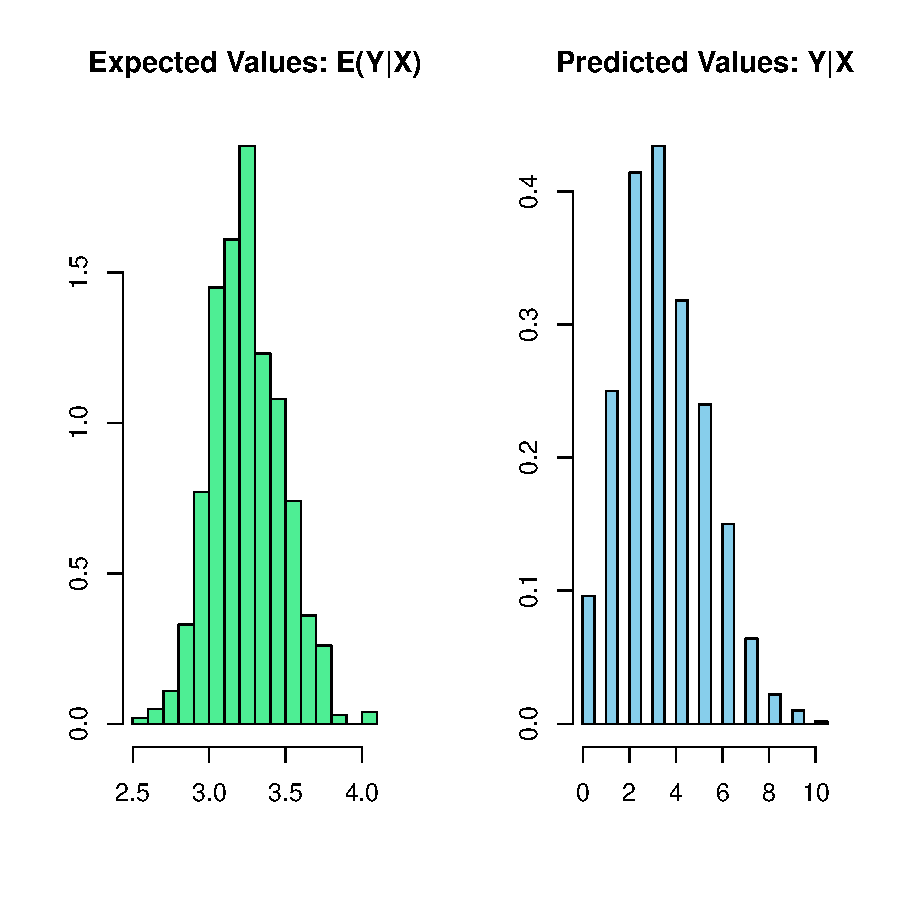
\includegraphics{vigpics/poisson-ExamplePlot}
\end{center}

\subsubsection{Model}
Let $Y_i$ be the number of independent events that occur during a
fixed time period. This variable can take any non-negative integer.

\begin{itemize}
\item The Poisson distribution has \emph{stochastic component}
  \begin{equation*}
    Y_i \; \sim \; \textrm{Poisson}(\lambda_i),
  \end{equation*}
  where $\lambda_i$ is the mean and variance parameter.
  
\item The \emph{systematic component} is 
  \begin{equation*}
    \lambda_i \; = \; \exp(x_i \beta),
  \end{equation*}
  where $x_i$ is the vector of explanatory variables, and $\beta$ is
  the vector of coefficients.
\end{itemize}

\subsubsection{Quantities of Interest}

\begin{itemize}
  
\item The expected value ({\tt qi\$ev}) is the mean of simulations
  from the stochastic component, $$E(Y) = \lambda_i =  \exp(x_i
  \beta),$$ given draws of $\beta$ from its sampling distribution.  
  
\item The predicted value ({\tt qi\$pr}) is a random draw from the
  poisson distribution defined by mean $\lambda_i$.

\item The first difference in the expected values ({\tt qi\$fd}) is given by:
\begin{equation*}
\textrm{FD} \; = \; E(Y | x_1) - E(Y \mid x)
\end{equation*}
\item In conditional prediction models, the average expected treatment
  effect ({\tt att.ev}) for the treatment group is 
    \begin{equation*} \frac{1}{\sum_{i=1}^n t_i}\sum_{i:t_i=1}^n \left\{ Y_i(t_i=1) -
      E[Y_i(t_i=0)] \right\},
    \end{equation*} 
    where $t_i$ is a binary explanatory variable defining the treatment
    ($t_i=1$) and control ($t_i=0$) groups.  Variation in the
    simulations are due to uncertainty in simulating $E[Y_i(t_i=0)]$,
    the counterfactual expected value of $Y_i$ for observations in the
    treatment group, under the assumption that everything stays the
    same except that the treatment indicator is switched to $t_i=0$.

\item In conditional prediction models, the average predicted treatment
  effect ({\tt att.pr}) for the treatment group is 
    \begin{equation*} \frac{1}{\sum_{i=1}^n t_i}\sum_{i:t_i=1}^n \left\{ Y_i(t_i=1) -
      \widehat{Y_i(t_i=0)} \right\},
    \end{equation*} 
    where $t_i$ is a binary explanatory variable defining the
    treatment ($t_i=1$) and control ($t_i=0$) groups.  Variation in
    the simulations are due to uncertainty in simulating
    $\widehat{Y_i(t_i=0)}$, the counterfactual predicted value of
    $Y_i$ for observations in the treatment group, under the
    assumption that everything stays the same except that the
    treatment indicator is switched to $t_i=0$.
\end{itemize}

\subsubsection{Output Values}

The output of each Zelig command contains useful information which you
may view.  For example, if you run \texttt{z.out <- zelig(y \~\,
  x, model = "poisson", data)}, then you may examine the available
information in \texttt{z.out} by using \texttt{names(z.out)},
see the {\tt coefficients} by using {\tt z.out\$coefficients}, and
a default summary of information through \texttt{summary(z.out)}.
Other elements available through the {\tt \$} operator are listed
below.

\begin{itemize}
\item From the {\tt zelig()} output object {\tt z.out}, you may extract:
   \begin{itemize}
   \item {\tt coefficients}: parameter estimates for the explanatory
     variables.
   \item {\tt residuals}: the working residuals in the final iteration
     of the IWLS fit.
   \item {\tt fitted.values}: a vector of the fitted values for the systemic
     component $\lambda$.  
   \item {\tt linear.predictors}: a vector of $x_{i}\beta$.  
   \item {\tt aic}: Akaike's Information Criterion (minus twice the
     maximized log-likelihood plus twice the number of coefficients).
   \item {\tt df.residual}: the residual degrees of freedom.
   \item {\tt df.null}: the residual degrees of freedom for the null
     model.
   \item {\tt zelig.data}: the input data frame if {\tt save.data = TRUE}.  
   \end{itemize}

\item From {\tt summary(z.out)}, you may extract: 
   \begin{itemize}
   \item {\tt coefficients}: the parameter estimates with their
     associated standard errors, $p$-values, and $t$-statistics.
   \item{\tt cov.scaled}: a $k \times k$ matrix of scaled covariances.
   \item{\tt cov.unscaled}: a $k \times k$ matrix of unscaled
     covariances.  
   \end{itemize}

\item From the {\tt sim()} output object {\tt s.out}, you may extract
  quantities of interest arranged as matrices indexed by simulation
  $\times$ {\tt x}-observation (for more than one {\tt x}-observation).
  Available quantities are:

   \begin{itemize}
   \item {\tt qi\$ev}: the simulated expected values given the
     specified values of {\tt x}.
   \item {\tt qi\$pr}: the simulated predicted values drawn from the
     distributions defined by $\lambda_i$.
   \item {\tt qi\$fd}: the simulated first differences in the expected
     values given the specified values of {\tt x} and {\tt x1}.
   \item {\tt qi\$att.ev}: the simulated average expected treatment
     effect for the treated from conditional prediction models.  
   \item {\tt qi\$att.pr}: the simulated average predicted treatment
     effect for the treated from conditional prediction models.  
   \end{itemize}
\end{itemize}

\subsection* {How to Cite} 


\include{zinput}
%\VignetteIndexEntry{Poisson Regression for Event Count Dependent Variables}
%\VignetteDepends{Zelig, stats}
%\VignetteKeyWords{model, poisson,regression, count}
%\VignettePackage{Zelig}
\usepackage{Sweave}
\begin{document}
\nobibliography*


\section{{\tt poisson}: Poisson Regression for Event Count
Dependent Variables}\label{poisson}

Use the Poisson regression model if the observations of your dependent
variable represents the number of independent events that occur during
a fixed period of time (see the negative binomial model, \Sref{negbin},
for over-dispersed event counts.)  For a Bayesian implementation of
this model, see \Sref{poisson.bayes}.  

\subsubsection{Syntax}

\begin{verbatim}
> z.out <- zelig(Y ~ X1 + X2, model = "poisson", data = mydata)
> x.out <- setx(z.out)
> s.out <- sim(z.out, x = x.out)
\end{verbatim}

\subsubsection{Additional Inputs} 

In addition to the standard inputs, {\tt zelig()} takes the following
additional options for poisson regression:  
\begin{itemize}
\item {\tt robust}: defaults to {\tt FALSE}.  If {\tt TRUE} is
selected, {\tt zelig()} computes robust standard errors via the {\tt
sandwich} package (see \cite{Zeileis04}).  The default type of robust
standard error is heteroskedastic and autocorrelation consistent (HAC),
and assumes that observations are ordered by time index.

In addition, {\tt robust} may be a list with the following options:  
\begin{itemize}
\item {\tt method}:  Choose from 
\begin{itemize}
\item {\tt "vcovHAC"}: (default if {\tt robust = TRUE}) HAC standard
errors. 
\item {\tt "kernHAC"}: HAC standard errors using the
weights given in \cite{Andrews91}. 
\item {\tt "weave"}: HAC standard errors using the
weights given in \cite{LumHea99}.  
\end{itemize}  
\item {\tt order.by}: defaults to {\tt NULL} (the observations are
chronologically ordered as in the original data).  Optionally, you may
specify a vector of weights (either as {\tt order.by = z}, where {\tt
z} exists outside the data frame; or as {\tt order.by = \~{}z}, where
{\tt z} is a variable in the data frame).  The observations are
chronologically ordered by the size of {\tt z}.
\item {\tt \dots}:  additional options passed to the functions 
specified in {\tt method}.   See the {\tt sandwich} library and
\cite{Zeileis04} for more options.   
\end{itemize}
\end{itemize}

\subsubsection{Example}

Load sample data:  
\begin{Schunk}
\begin{Sinput}
> data(sanction)
\end{Sinput}
\end{Schunk}
Estimate Poisson model:  
\begin{Schunk}
\begin{Sinput}
> z.out <- zelig(num ~ target + coop, model = "poisson", data = sanction)
\end{Sinput}
\end{Schunk}
\begin{Schunk}
\begin{Sinput}
> summary(z.out)
\end{Sinput}
\end{Schunk}
Set values for the explanatory variables to their default mean values:  
\begin{Schunk}
\begin{Sinput}
> x.out <- setx(z.out)
\end{Sinput}
\end{Schunk}
Simulate fitted values:  
\begin{Schunk}
\begin{Sinput}
> s.out <- sim(z.out, x = x.out)
\end{Sinput}
\end{Schunk}
\begin{Schunk}
\begin{Sinput}
> summary(s.out)
\end{Sinput}
\end{Schunk}
\begin{center}
\begin{Schunk}
\begin{Sinput}
> plot(s.out)
\end{Sinput}
\end{Schunk}
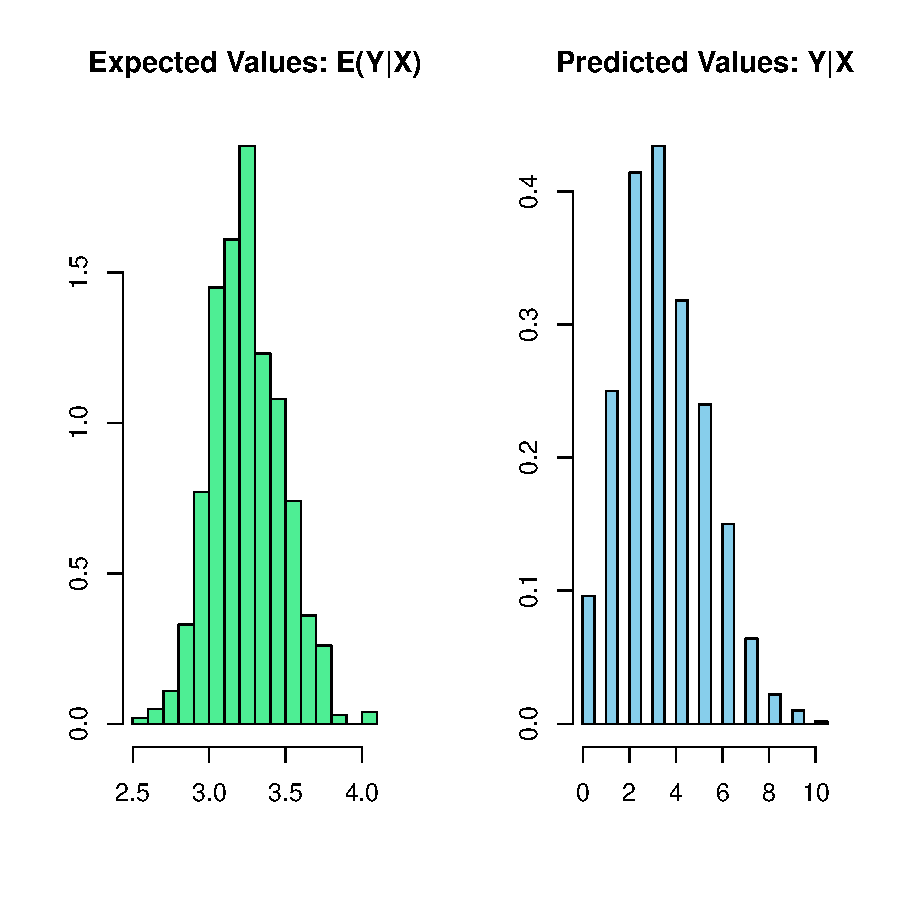
\includegraphics{vigpics/poisson-ExamplePlot}
\end{center}

\subsubsection{Model}
Let $Y_i$ be the number of independent events that occur during a
fixed time period. This variable can take any non-negative integer.

\begin{itemize}
\item The Poisson distribution has \emph{stochastic component}
  \begin{equation*}
    Y_i \; \sim \; \textrm{Poisson}(\lambda_i),
  \end{equation*}
  where $\lambda_i$ is the mean and variance parameter.
  
\item The \emph{systematic component} is 
  \begin{equation*}
    \lambda_i \; = \; \exp(x_i \beta),
  \end{equation*}
  where $x_i$ is the vector of explanatory variables, and $\beta$ is
  the vector of coefficients.
\end{itemize}

\subsubsection{Quantities of Interest}

\begin{itemize}
  
\item The expected value ({\tt qi\$ev}) is the mean of simulations
  from the stochastic component, $$E(Y) = \lambda_i =  \exp(x_i
  \beta),$$ given draws of $\beta$ from its sampling distribution.  
  
\item The predicted value ({\tt qi\$pr}) is a random draw from the
  poisson distribution defined by mean $\lambda_i$.

\item The first difference in the expected values ({\tt qi\$fd}) is given by:
\begin{equation*}
\textrm{FD} \; = \; E(Y | x_1) - E(Y \mid x)
\end{equation*}
\item In conditional prediction models, the average expected treatment
  effect ({\tt att.ev}) for the treatment group is 
    \begin{equation*} \frac{1}{\sum_{i=1}^n t_i}\sum_{i:t_i=1}^n \left\{ Y_i(t_i=1) -
      E[Y_i(t_i=0)] \right\},
    \end{equation*} 
    where $t_i$ is a binary explanatory variable defining the treatment
    ($t_i=1$) and control ($t_i=0$) groups.  Variation in the
    simulations are due to uncertainty in simulating $E[Y_i(t_i=0)]$,
    the counterfactual expected value of $Y_i$ for observations in the
    treatment group, under the assumption that everything stays the
    same except that the treatment indicator is switched to $t_i=0$.

\item In conditional prediction models, the average predicted treatment
  effect ({\tt att.pr}) for the treatment group is 
    \begin{equation*} \frac{1}{\sum_{i=1}^n t_i}\sum_{i:t_i=1}^n \left\{ Y_i(t_i=1) -
      \widehat{Y_i(t_i=0)} \right\},
    \end{equation*} 
    where $t_i$ is a binary explanatory variable defining the
    treatment ($t_i=1$) and control ($t_i=0$) groups.  Variation in
    the simulations are due to uncertainty in simulating
    $\widehat{Y_i(t_i=0)}$, the counterfactual predicted value of
    $Y_i$ for observations in the treatment group, under the
    assumption that everything stays the same except that the
    treatment indicator is switched to $t_i=0$.
\end{itemize}

\subsubsection{Output Values}

The output of each Zelig command contains useful information which you
may view.  For example, if you run \texttt{z.out <- zelig(y \~\,
  x, model = "poisson", data)}, then you may examine the available
information in \texttt{z.out} by using \texttt{names(z.out)},
see the {\tt coefficients} by using {\tt z.out\$coefficients}, and
a default summary of information through \texttt{summary(z.out)}.
Other elements available through the {\tt \$} operator are listed
below.

\begin{itemize}
\item From the {\tt zelig()} output object {\tt z.out}, you may extract:
   \begin{itemize}
   \item {\tt coefficients}: parameter estimates for the explanatory
     variables.
   \item {\tt residuals}: the working residuals in the final iteration
     of the IWLS fit.
   \item {\tt fitted.values}: a vector of the fitted values for the systemic
     component $\lambda$.  
   \item {\tt linear.predictors}: a vector of $x_{i}\beta$.  
   \item {\tt aic}: Akaike's Information Criterion (minus twice the
     maximized log-likelihood plus twice the number of coefficients).
   \item {\tt df.residual}: the residual degrees of freedom.
   \item {\tt df.null}: the residual degrees of freedom for the null
     model.
   \item {\tt zelig.data}: the input data frame if {\tt save.data = TRUE}.  
   \end{itemize}

\item From {\tt summary(z.out)}, you may extract: 
   \begin{itemize}
   \item {\tt coefficients}: the parameter estimates with their
     associated standard errors, $p$-values, and $t$-statistics.
   \item{\tt cov.scaled}: a $k \times k$ matrix of scaled covariances.
   \item{\tt cov.unscaled}: a $k \times k$ matrix of unscaled
     covariances.  
   \end{itemize}

\item From the {\tt sim()} output object {\tt s.out}, you may extract
  quantities of interest arranged as matrices indexed by simulation
  $\times$ {\tt x}-observation (for more than one {\tt x}-observation).
  Available quantities are:

   \begin{itemize}
   \item {\tt qi\$ev}: the simulated expected values given the
     specified values of {\tt x}.
   \item {\tt qi\$pr}: the simulated predicted values drawn from the
     distributions defined by $\lambda_i$.
   \item {\tt qi\$fd}: the simulated first differences in the expected
     values given the specified values of {\tt x} and {\tt x1}.
   \item {\tt qi\$att.ev}: the simulated average expected treatment
     effect for the treated from conditional prediction models.  
   \item {\tt qi\$att.pr}: the simulated average predicted treatment
     effect for the treated from conditional prediction models.  
   \end{itemize}
\end{itemize}

\subsection* {How to Cite} 

\input{cites/poisson}
\input{citeZelig}

\subsection* {See also}
The poisson model is part of the stats package by \citet{VenRip02}.
Advanced users may wish to refer to \texttt{help(glm)} and
\texttt{help(family)}, as well as \cite{McCNel89}. Robust standard
errors are implemented via the sandwich package by \citet{Zeileis04}.
Sample data are from \cite{Martin92}.

\bibliographystyle{asa}
\bibliography{gk,gkpubs}
 \end{document}


%%% Local Variables: 
%%% mode: latex
%%% TeX-master: t
%%% End: 

To cite Zelig as a whole, please reference these two sources:
\begin{verse}
  Kosuke Imai, Gary King, and Olivia Lau. 2007. ``Zelig: Everyone's
  Statistical Software,'' \url{http://GKing.harvard.edu/zelig}.
\end{verse}
\begin{verse}
Imai, Kosuke, Gary King, and Olivia Lau. (2008). ``Toward A Common Framework for Statistical Analysis and Development.'' Journal of Computational and Graphical Statistics, Vol. 17, No. 4 (December), pp. 892-913. 
\end{verse}


\subsection* {See also}
The poisson model is part of the stats package by \citet{VenRip02}.
Advanced users may wish to refer to \texttt{help(glm)} and
\texttt{help(family)}, as well as \cite{McCNel89}. Robust standard
errors are implemented via the sandwich package by \citet{Zeileis04}.
Sample data are from \cite{Martin92}.

\bibliographystyle{asa}
\bibliography{gk,gkpubs}
 \end{document}


%%% Local Variables: 
%%% mode: latex
%%% TeX-master: t
%%% End: 

To cite Zelig as a whole, please reference these two sources:
\begin{verse}
  Kosuke Imai, Gary King, and Olivia Lau. 2007. ``Zelig: Everyone's
  Statistical Software,'' \url{http://GKing.harvard.edu/zelig}.
\end{verse}
\begin{verse}
Imai, Kosuke, Gary King, and Olivia Lau. (2008). ``Toward A Common Framework for Statistical Analysis and Development.'' Journal of Computational and Graphical Statistics, Vol. 17, No. 4 (December), pp. 892-913. 
\end{verse}


\subsection* {See also}
The poisson model is part of the stats package by \citet{VenRip02}.
Advanced users may wish to refer to \texttt{help(glm)} and
\texttt{help(family)}, as well as \cite{McCNel89}. Robust standard
errors are implemented via the sandwich package by \citet{Zeileis04}.
Sample data are from \cite{Martin92}.

\bibliographystyle{asa}
\bibliography{gk,gkpubs}
 \end{document}


%%% Local Variables: 
%%% mode: latex
%%% TeX-master: t
%%% End: 


\documentclass[oneside,letterpaper,12pt]{book}
\usepackage{Rd}
%\usepackage{Sweave}
%\usepackage{/usr/lib64/R/share/texmf/Sweave}
%\usepackage{/usr/share/R/texmf/Sweave}
\usepackage{bibentry}
\usepackage{upquote}
\usepackage{graphicx}
\usepackage{natbib}
\usepackage[reqno]{amsmath}
\usepackage{amssymb}
\usepackage{amsfonts}
\usepackage{amsmath}
\usepackage{verbatim}
\usepackage{epsf}
\usepackage{url}
\usepackage{html}
\usepackage{dcolumn}
\usepackage{multirow}
\usepackage{fullpage}
\usepackage{lscape}
\usepackage[all]{xy}

\usepackage{csquotes}
% \usepackage[pdftex, bookmarksopen=true,bookmarksnumbered=true,
%   linkcolor=webred]{hyperref}
\bibpunct{(}{)}{;}{a}{}{,}
\newcolumntype{.}{D{.}{.}{-1}}
\newcolumntype{d}[1]{D{.}{.}{#1}}
\htmladdtonavigation{
  \htmladdnormallink{%
    \htmladdimg{http://gking.harvard.edu/pics/home.gif}}
  {http://gking.harvard.edu/}}
\newcommand{\MatchIt}{{\sc MatchIt}}
\newcommand{\hlink}{\htmladdnormallink}
\newcommand{\Sref}[1]{Section~\ref{#1}}
\newcommand{\fullrvers}{2.5.1}
\newcommand{\rvers}{2.5}
\newcommand{\rwvers}{R-2.5.1}
%\renewcommand{\bibentry}{\citealt}

\bodytext{ BACKGROUND="http://gking.harvard.edu/pics/temple.jpg"}
\setcounter{tocdepth}{2}

%\VignetteIndexEntry{Probit Regression for Dichotomous Dependent Variables}
%\VignetteDepends{Zelig}
%\VignetteKeyWords{model, probit,regression,dichotomous, binary}
%\VignettePackage{Zelig}
\usepackage{Sweave}
\begin{document}
\nobibliography*


\section{{\tt probit}: Probit Regression for Dichotomous Dependent Variables}\label{probit}

Use probit regression to model binary dependent variables
specified as a function of a set of explanatory variables.  For a
Bayesian implementation of this model, see \Sref{probit.bayes}.  

\subsubsection{Syntax}
\begin{verbatim}
> z.out <- zelig(Y ~ X1 + X2, model = "probit", data = mydata)
> x.out <- setx(z.out)
> s.out <- sim(z.out, x = x.out, x1 = NULL)
\end{verbatim}

\subsubsection{Additional Inputs} 

In addition to the standard inputs, {\tt zelig()} takes the following
additional options for probit regression:  
\begin{itemize}
\item {\tt robust}: defaults to {\tt FALSE}.  If {\tt TRUE} is
selected, {\tt zelig()} computes robust standard errors via the {\tt
sandwich} package (see \cite{Zeileis04}).  The default type of robust
standard error is heteroskedastic and autocorrelation consistent (HAC),
and assumes that observations are ordered by time index.

In addition, {\tt robust} may be a list with the following options:  
\begin{itemize}
\item {\tt method}:  Choose from 
\begin{itemize}
\item {\tt "vcovHAC"}: (default if {\tt robust = TRUE}) HAC standard
errors. 
\item {\tt "kernHAC"}: HAC standard errors using the
weights given in \cite{Andrews91}. 
\item {\tt "weave"}: HAC standard errors using the
weights given in \cite{LumHea99}.  
\end{itemize}  
\item {\tt order.by}: defaults to {\tt NULL} (the observations are
chronologically ordered as in the original data).  Optionally, you may
specify a vector of weights (either as {\tt order.by = z}, where {\tt
z} exists outside the data frame; or as {\tt order.by = \~{}z}, where
{\tt z} is a variable in the data frame).  The observations are
chronologically ordered by the size of {\tt z}.
\item {\tt \dots}:  additional options passed to the functions 
specified in {\tt method}.   See the {\tt sandwich} library and
\cite{Zeileis04} for more options.   
\end{itemize}
\end{itemize}

\subsubsection{Examples}
Attach the sample turnout dataset:
\begin{Schunk}
\begin{Sinput}
> data(turnout)
\end{Sinput}
\end{Schunk}
Estimate parameter values for the probit regression:
\begin{Schunk}
\begin{Sinput}
> z.out <- zelig(vote ~ race + educate, model = "probit", data = turnout)
\end{Sinput}
\end{Schunk}
\begin{Schunk}
\begin{Sinput}
> summary(z.out)
\end{Sinput}
\end{Schunk}
Set values for the explanatory variables to their default values.
\begin{Schunk}
\begin{Sinput}
> x.out <- setx(z.out)
\end{Sinput}
\end{Schunk}
Simulate quantities of interest from the posterior distribution.
\begin{Schunk}
\begin{Sinput}
> s.out <- sim(z.out, x = x.out)
\end{Sinput}
\end{Schunk}
\begin{Schunk}
\begin{Sinput}
> summary(s.out)
\end{Sinput}
\end{Schunk}

\subsubsection{Model}
Let $Y_i$ be the observed binary dependent variable for observation
$i$ which takes the value of either 0 or 1.
\begin{itemize}
\item The \emph{stochastic component} is given by  
\begin{equation*}
Y_i \; \sim \; \textrm{Bernoulli}(\pi_i), 
\end{equation*}
where $\pi_i=\Pr(Y_i=1)$.

\item The \emph{systematic component} is 
\begin{equation*}
  \pi_i \; = \; \Phi (x_i \beta)
\end{equation*}
where $\Phi(\mu)$ is the cumulative distribution function of the
Normal distribution with mean 0 and unit variance.
\end{itemize}

\subsubsection{Quantities of Interest}

\begin{itemize}

\item The expected value ({\tt qi\$ev}) is a simulation of predicted
  probability of success $$E(Y) = \pi_i = \Phi(x_i
  \beta),$$ given a draw of $\beta$ from its sampling distribution.  

\item The predicted value ({\tt qi\$pr}) is a draw from a Bernoulli
  distribution with mean $\pi_i$.  
  
\item The first difference ({\tt qi\$fd}) in expected values is
  defined as
\begin{equation*}
\textrm{FD} = \Pr(Y = 1 \mid x_1) - \Pr(Y = 1 \mid x).
\end{equation*}

\item The risk ratio ({\tt qi\$rr}) is defined as
\begin{equation*}
\textrm{RR} = \Pr(Y = 1 \mid x_1) / \Pr(Y = 1 \mid x).
\end{equation*}

\item In conditional prediction models, the average expected treatment
  effect ({\tt att.ev}) for the treatment group is 
    \begin{equation*} \frac{1}{\sum_{i=1}^n t_i}\sum_{i:t_i=1}^n \left\{ Y_i(t_i=1) -
      E[Y_i(t_i=0)] \right\},
    \end{equation*} 
    where $t_i$ is a binary explanatory variable defining the treatment
    ($t_i=1$) and control ($t_i=0$) groups.  Variation in the
    simulations are due to uncertainty in simulating $E[Y_i(t_i=0)]$,
    the counterfactual expected value of $Y_i$ for observations in the
    treatment group, under the assumption that everything stays the
    same except that the treatment indicator is switched to $t_i=0$.

\item In conditional prediction models, the average predicted treatment
  effect ({\tt att.pr}) for the treatment group is 
    \begin{equation*} \frac{1}{\sum_{i=1}^n t_i}\sum_{i:t_i=1}^n \left\{ Y_i(t_i=1) -
      \widehat{Y_i(t_i=0)} \right\},
    \end{equation*} 
    where $t_i$ is a binary explanatory variable defining the
    treatment ($t_i=1$) and control ($t_i=0$) groups.  Variation in
    the simulations are due to uncertainty in simulating
    $\widehat{Y_i(t_i=0)}$, the counterfactual predicted value of
    $Y_i$ for observations in the treatment group, under the
    assumption that everything stays the same except that the
    treatment indicator is switched to $t_i=0$.
\end{itemize}

\subsubsection{Output Values}

The output of each Zelig command contains useful information which you
may view.  For example, if you run \texttt{z.out <- zelig(y \~\,
  x, model = "probit", data)}, then you may examine the available
information in \texttt{z.out} by using \texttt{names(z.out)},
see the {\tt coefficients} by using {\tt z.out\$coefficients}, and
a default summary of information through \texttt{summary(z.out)}.
Other elements available through the {\tt \$} operator are listed
below.

\begin{itemize}
\item From the {\tt zelig()} output object {\tt z.out}, you may extract:
   \begin{itemize}
   \item {\tt coefficients}: parameter estimates for the explanatory
     variables.
   \item {\tt residuals}: the working residuals in the final iteration
     of the IWLS fit.
   \item {\tt fitted.values}: a vector of the in-sample fitted values.
   \item {\tt linear.predictors}: a vector of $x_{i}\beta$.  
   \item {\tt aic}: Akaike's Information Criterion (minus twice the
     maximized log-likelihood plus twice the number of coefficients).
   \item {\tt df.residual}: the residual degrees of freedom.
   \item {\tt df.null}: the residual degrees of freedom for the null
     model.
   \item {\tt data}: the name of the input data frame.  
   \end{itemize}

\item From {\tt summary(z.out)}, you may extract: 
   \begin{itemize}
   \item {\tt coefficients}: the parameter estimates with their
     associated standard errors, $p$-values, and $t$-statistics.
   \item{\tt cov.scaled}: a $k \times k$ matrix of scaled covariances.
   \item{\tt cov.unscaled}: a $k \times k$ matrix of unscaled
     covariances.  
   \end{itemize}

\item From the {\tt sim()} output object {\tt s.out}, you may extract
  quantities of interest arranged as matrices indexed by simulation
  $\times$ {\tt x}-observation (for more than one {\tt x}-observation).
  Available quantities are:

   \begin{itemize}
   \item {\tt qi\$ev}: the simulated expected values, or predicted
     probabilities, for the specified values of {\tt x}.
   \item {\tt qi\$pr}: the simulated predicted values drawn from the
     distributions defined by the predicted probabilities.  
   \item {\tt qi\$fd}: the simulated first differences in the predicted
     probabilities for the values specified in {\tt x} and {\tt x1}.
   \item {\tt qi\$rr}: the simulated risk ratio for the predicted
     probabilities simulated from {\tt x} and {\tt x1}.
   \item {\tt qi\$att.ev}: the simulated average expected treatment
     effect for the treated from conditional prediction models.  
   \item {\tt qi\$att.pr}: the simulated average predicted treatment
     effect for the treated from conditional prediction models.  
   \end{itemize}
\end{itemize}


\subsection* {How to Cite} 


\documentclass[oneside,letterpaper,12pt]{book}
\usepackage{Rd}
%\usepackage{Sweave}
%\usepackage{/usr/lib64/R/share/texmf/Sweave}
%\usepackage{/usr/share/R/texmf/Sweave}
\usepackage{bibentry}
\usepackage{upquote}
\usepackage{graphicx}
\usepackage{natbib}
\usepackage[reqno]{amsmath}
\usepackage{amssymb}
\usepackage{amsfonts}
\usepackage{amsmath}
\usepackage{verbatim}
\usepackage{epsf}
\usepackage{url}
\usepackage{html}
\usepackage{dcolumn}
\usepackage{multirow}
\usepackage{fullpage}
\usepackage{lscape}
\usepackage[all]{xy}

\usepackage{csquotes}
% \usepackage[pdftex, bookmarksopen=true,bookmarksnumbered=true,
%   linkcolor=webred]{hyperref}
\bibpunct{(}{)}{;}{a}{}{,}
\newcolumntype{.}{D{.}{.}{-1}}
\newcolumntype{d}[1]{D{.}{.}{#1}}
\htmladdtonavigation{
  \htmladdnormallink{%
    \htmladdimg{http://gking.harvard.edu/pics/home.gif}}
  {http://gking.harvard.edu/}}
\newcommand{\MatchIt}{{\sc MatchIt}}
\newcommand{\hlink}{\htmladdnormallink}
\newcommand{\Sref}[1]{Section~\ref{#1}}
\newcommand{\fullrvers}{2.5.1}
\newcommand{\rvers}{2.5}
\newcommand{\rwvers}{R-2.5.1}
%\renewcommand{\bibentry}{\citealt}

\bodytext{ BACKGROUND="http://gking.harvard.edu/pics/temple.jpg"}
\setcounter{tocdepth}{2}

%\VignetteIndexEntry{Probit Regression for Dichotomous Dependent Variables}
%\VignetteDepends{Zelig}
%\VignetteKeyWords{model, probit,regression,dichotomous, binary}
%\VignettePackage{Zelig}
\usepackage{Sweave}
\begin{document}
\nobibliography*


\section{{\tt probit}: Probit Regression for Dichotomous Dependent Variables}\label{probit}

Use probit regression to model binary dependent variables
specified as a function of a set of explanatory variables.  For a
Bayesian implementation of this model, see \Sref{probit.bayes}.  

\subsubsection{Syntax}
\begin{verbatim}
> z.out <- zelig(Y ~ X1 + X2, model = "probit", data = mydata)
> x.out <- setx(z.out)
> s.out <- sim(z.out, x = x.out, x1 = NULL)
\end{verbatim}

\subsubsection{Additional Inputs} 

In addition to the standard inputs, {\tt zelig()} takes the following
additional options for probit regression:  
\begin{itemize}
\item {\tt robust}: defaults to {\tt FALSE}.  If {\tt TRUE} is
selected, {\tt zelig()} computes robust standard errors via the {\tt
sandwich} package (see \cite{Zeileis04}).  The default type of robust
standard error is heteroskedastic and autocorrelation consistent (HAC),
and assumes that observations are ordered by time index.

In addition, {\tt robust} may be a list with the following options:  
\begin{itemize}
\item {\tt method}:  Choose from 
\begin{itemize}
\item {\tt "vcovHAC"}: (default if {\tt robust = TRUE}) HAC standard
errors. 
\item {\tt "kernHAC"}: HAC standard errors using the
weights given in \cite{Andrews91}. 
\item {\tt "weave"}: HAC standard errors using the
weights given in \cite{LumHea99}.  
\end{itemize}  
\item {\tt order.by}: defaults to {\tt NULL} (the observations are
chronologically ordered as in the original data).  Optionally, you may
specify a vector of weights (either as {\tt order.by = z}, where {\tt
z} exists outside the data frame; or as {\tt order.by = \~{}z}, where
{\tt z} is a variable in the data frame).  The observations are
chronologically ordered by the size of {\tt z}.
\item {\tt \dots}:  additional options passed to the functions 
specified in {\tt method}.   See the {\tt sandwich} library and
\cite{Zeileis04} for more options.   
\end{itemize}
\end{itemize}

\subsubsection{Examples}
Attach the sample turnout dataset:
\begin{Schunk}
\begin{Sinput}
> data(turnout)
\end{Sinput}
\end{Schunk}
Estimate parameter values for the probit regression:
\begin{Schunk}
\begin{Sinput}
> z.out <- zelig(vote ~ race + educate, model = "probit", data = turnout)
\end{Sinput}
\end{Schunk}
\begin{Schunk}
\begin{Sinput}
> summary(z.out)
\end{Sinput}
\end{Schunk}
Set values for the explanatory variables to their default values.
\begin{Schunk}
\begin{Sinput}
> x.out <- setx(z.out)
\end{Sinput}
\end{Schunk}
Simulate quantities of interest from the posterior distribution.
\begin{Schunk}
\begin{Sinput}
> s.out <- sim(z.out, x = x.out)
\end{Sinput}
\end{Schunk}
\begin{Schunk}
\begin{Sinput}
> summary(s.out)
\end{Sinput}
\end{Schunk}

\subsubsection{Model}
Let $Y_i$ be the observed binary dependent variable for observation
$i$ which takes the value of either 0 or 1.
\begin{itemize}
\item The \emph{stochastic component} is given by  
\begin{equation*}
Y_i \; \sim \; \textrm{Bernoulli}(\pi_i), 
\end{equation*}
where $\pi_i=\Pr(Y_i=1)$.

\item The \emph{systematic component} is 
\begin{equation*}
  \pi_i \; = \; \Phi (x_i \beta)
\end{equation*}
where $\Phi(\mu)$ is the cumulative distribution function of the
Normal distribution with mean 0 and unit variance.
\end{itemize}

\subsubsection{Quantities of Interest}

\begin{itemize}

\item The expected value ({\tt qi\$ev}) is a simulation of predicted
  probability of success $$E(Y) = \pi_i = \Phi(x_i
  \beta),$$ given a draw of $\beta$ from its sampling distribution.  

\item The predicted value ({\tt qi\$pr}) is a draw from a Bernoulli
  distribution with mean $\pi_i$.  
  
\item The first difference ({\tt qi\$fd}) in expected values is
  defined as
\begin{equation*}
\textrm{FD} = \Pr(Y = 1 \mid x_1) - \Pr(Y = 1 \mid x).
\end{equation*}

\item The risk ratio ({\tt qi\$rr}) is defined as
\begin{equation*}
\textrm{RR} = \Pr(Y = 1 \mid x_1) / \Pr(Y = 1 \mid x).
\end{equation*}

\item In conditional prediction models, the average expected treatment
  effect ({\tt att.ev}) for the treatment group is 
    \begin{equation*} \frac{1}{\sum_{i=1}^n t_i}\sum_{i:t_i=1}^n \left\{ Y_i(t_i=1) -
      E[Y_i(t_i=0)] \right\},
    \end{equation*} 
    where $t_i$ is a binary explanatory variable defining the treatment
    ($t_i=1$) and control ($t_i=0$) groups.  Variation in the
    simulations are due to uncertainty in simulating $E[Y_i(t_i=0)]$,
    the counterfactual expected value of $Y_i$ for observations in the
    treatment group, under the assumption that everything stays the
    same except that the treatment indicator is switched to $t_i=0$.

\item In conditional prediction models, the average predicted treatment
  effect ({\tt att.pr}) for the treatment group is 
    \begin{equation*} \frac{1}{\sum_{i=1}^n t_i}\sum_{i:t_i=1}^n \left\{ Y_i(t_i=1) -
      \widehat{Y_i(t_i=0)} \right\},
    \end{equation*} 
    where $t_i$ is a binary explanatory variable defining the
    treatment ($t_i=1$) and control ($t_i=0$) groups.  Variation in
    the simulations are due to uncertainty in simulating
    $\widehat{Y_i(t_i=0)}$, the counterfactual predicted value of
    $Y_i$ for observations in the treatment group, under the
    assumption that everything stays the same except that the
    treatment indicator is switched to $t_i=0$.
\end{itemize}

\subsubsection{Output Values}

The output of each Zelig command contains useful information which you
may view.  For example, if you run \texttt{z.out <- zelig(y \~\,
  x, model = "probit", data)}, then you may examine the available
information in \texttt{z.out} by using \texttt{names(z.out)},
see the {\tt coefficients} by using {\tt z.out\$coefficients}, and
a default summary of information through \texttt{summary(z.out)}.
Other elements available through the {\tt \$} operator are listed
below.

\begin{itemize}
\item From the {\tt zelig()} output object {\tt z.out}, you may extract:
   \begin{itemize}
   \item {\tt coefficients}: parameter estimates for the explanatory
     variables.
   \item {\tt residuals}: the working residuals in the final iteration
     of the IWLS fit.
   \item {\tt fitted.values}: a vector of the in-sample fitted values.
   \item {\tt linear.predictors}: a vector of $x_{i}\beta$.  
   \item {\tt aic}: Akaike's Information Criterion (minus twice the
     maximized log-likelihood plus twice the number of coefficients).
   \item {\tt df.residual}: the residual degrees of freedom.
   \item {\tt df.null}: the residual degrees of freedom for the null
     model.
   \item {\tt data}: the name of the input data frame.  
   \end{itemize}

\item From {\tt summary(z.out)}, you may extract: 
   \begin{itemize}
   \item {\tt coefficients}: the parameter estimates with their
     associated standard errors, $p$-values, and $t$-statistics.
   \item{\tt cov.scaled}: a $k \times k$ matrix of scaled covariances.
   \item{\tt cov.unscaled}: a $k \times k$ matrix of unscaled
     covariances.  
   \end{itemize}

\item From the {\tt sim()} output object {\tt s.out}, you may extract
  quantities of interest arranged as matrices indexed by simulation
  $\times$ {\tt x}-observation (for more than one {\tt x}-observation).
  Available quantities are:

   \begin{itemize}
   \item {\tt qi\$ev}: the simulated expected values, or predicted
     probabilities, for the specified values of {\tt x}.
   \item {\tt qi\$pr}: the simulated predicted values drawn from the
     distributions defined by the predicted probabilities.  
   \item {\tt qi\$fd}: the simulated first differences in the predicted
     probabilities for the values specified in {\tt x} and {\tt x1}.
   \item {\tt qi\$rr}: the simulated risk ratio for the predicted
     probabilities simulated from {\tt x} and {\tt x1}.
   \item {\tt qi\$att.ev}: the simulated average expected treatment
     effect for the treated from conditional prediction models.  
   \item {\tt qi\$att.pr}: the simulated average predicted treatment
     effect for the treated from conditional prediction models.  
   \end{itemize}
\end{itemize}


\subsection* {How to Cite} 


\include{zinput}
%\VignetteIndexEntry{Probit Regression for Dichotomous Dependent Variables}
%\VignetteDepends{Zelig}
%\VignetteKeyWords{model, probit,regression,dichotomous, binary}
%\VignettePackage{Zelig}
\usepackage{Sweave}
\begin{document}
\nobibliography*


\section{{\tt probit}: Probit Regression for Dichotomous Dependent Variables}\label{probit}

Use probit regression to model binary dependent variables
specified as a function of a set of explanatory variables.  For a
Bayesian implementation of this model, see \Sref{probit.bayes}.  

\subsubsection{Syntax}
\begin{verbatim}
> z.out <- zelig(Y ~ X1 + X2, model = "probit", data = mydata)
> x.out <- setx(z.out)
> s.out <- sim(z.out, x = x.out, x1 = NULL)
\end{verbatim}

\subsubsection{Additional Inputs} 

In addition to the standard inputs, {\tt zelig()} takes the following
additional options for probit regression:  
\begin{itemize}
\item {\tt robust}: defaults to {\tt FALSE}.  If {\tt TRUE} is
selected, {\tt zelig()} computes robust standard errors via the {\tt
sandwich} package (see \cite{Zeileis04}).  The default type of robust
standard error is heteroskedastic and autocorrelation consistent (HAC),
and assumes that observations are ordered by time index.

In addition, {\tt robust} may be a list with the following options:  
\begin{itemize}
\item {\tt method}:  Choose from 
\begin{itemize}
\item {\tt "vcovHAC"}: (default if {\tt robust = TRUE}) HAC standard
errors. 
\item {\tt "kernHAC"}: HAC standard errors using the
weights given in \cite{Andrews91}. 
\item {\tt "weave"}: HAC standard errors using the
weights given in \cite{LumHea99}.  
\end{itemize}  
\item {\tt order.by}: defaults to {\tt NULL} (the observations are
chronologically ordered as in the original data).  Optionally, you may
specify a vector of weights (either as {\tt order.by = z}, where {\tt
z} exists outside the data frame; or as {\tt order.by = \~{}z}, where
{\tt z} is a variable in the data frame).  The observations are
chronologically ordered by the size of {\tt z}.
\item {\tt \dots}:  additional options passed to the functions 
specified in {\tt method}.   See the {\tt sandwich} library and
\cite{Zeileis04} for more options.   
\end{itemize}
\end{itemize}

\subsubsection{Examples}
Attach the sample turnout dataset:
\begin{Schunk}
\begin{Sinput}
> data(turnout)
\end{Sinput}
\end{Schunk}
Estimate parameter values for the probit regression:
\begin{Schunk}
\begin{Sinput}
> z.out <- zelig(vote ~ race + educate, model = "probit", data = turnout)
\end{Sinput}
\end{Schunk}
\begin{Schunk}
\begin{Sinput}
> summary(z.out)
\end{Sinput}
\end{Schunk}
Set values for the explanatory variables to their default values.
\begin{Schunk}
\begin{Sinput}
> x.out <- setx(z.out)
\end{Sinput}
\end{Schunk}
Simulate quantities of interest from the posterior distribution.
\begin{Schunk}
\begin{Sinput}
> s.out <- sim(z.out, x = x.out)
\end{Sinput}
\end{Schunk}
\begin{Schunk}
\begin{Sinput}
> summary(s.out)
\end{Sinput}
\end{Schunk}

\subsubsection{Model}
Let $Y_i$ be the observed binary dependent variable for observation
$i$ which takes the value of either 0 or 1.
\begin{itemize}
\item The \emph{stochastic component} is given by  
\begin{equation*}
Y_i \; \sim \; \textrm{Bernoulli}(\pi_i), 
\end{equation*}
where $\pi_i=\Pr(Y_i=1)$.

\item The \emph{systematic component} is 
\begin{equation*}
  \pi_i \; = \; \Phi (x_i \beta)
\end{equation*}
where $\Phi(\mu)$ is the cumulative distribution function of the
Normal distribution with mean 0 and unit variance.
\end{itemize}

\subsubsection{Quantities of Interest}

\begin{itemize}

\item The expected value ({\tt qi\$ev}) is a simulation of predicted
  probability of success $$E(Y) = \pi_i = \Phi(x_i
  \beta),$$ given a draw of $\beta$ from its sampling distribution.  

\item The predicted value ({\tt qi\$pr}) is a draw from a Bernoulli
  distribution with mean $\pi_i$.  
  
\item The first difference ({\tt qi\$fd}) in expected values is
  defined as
\begin{equation*}
\textrm{FD} = \Pr(Y = 1 \mid x_1) - \Pr(Y = 1 \mid x).
\end{equation*}

\item The risk ratio ({\tt qi\$rr}) is defined as
\begin{equation*}
\textrm{RR} = \Pr(Y = 1 \mid x_1) / \Pr(Y = 1 \mid x).
\end{equation*}

\item In conditional prediction models, the average expected treatment
  effect ({\tt att.ev}) for the treatment group is 
    \begin{equation*} \frac{1}{\sum_{i=1}^n t_i}\sum_{i:t_i=1}^n \left\{ Y_i(t_i=1) -
      E[Y_i(t_i=0)] \right\},
    \end{equation*} 
    where $t_i$ is a binary explanatory variable defining the treatment
    ($t_i=1$) and control ($t_i=0$) groups.  Variation in the
    simulations are due to uncertainty in simulating $E[Y_i(t_i=0)]$,
    the counterfactual expected value of $Y_i$ for observations in the
    treatment group, under the assumption that everything stays the
    same except that the treatment indicator is switched to $t_i=0$.

\item In conditional prediction models, the average predicted treatment
  effect ({\tt att.pr}) for the treatment group is 
    \begin{equation*} \frac{1}{\sum_{i=1}^n t_i}\sum_{i:t_i=1}^n \left\{ Y_i(t_i=1) -
      \widehat{Y_i(t_i=0)} \right\},
    \end{equation*} 
    where $t_i$ is a binary explanatory variable defining the
    treatment ($t_i=1$) and control ($t_i=0$) groups.  Variation in
    the simulations are due to uncertainty in simulating
    $\widehat{Y_i(t_i=0)}$, the counterfactual predicted value of
    $Y_i$ for observations in the treatment group, under the
    assumption that everything stays the same except that the
    treatment indicator is switched to $t_i=0$.
\end{itemize}

\subsubsection{Output Values}

The output of each Zelig command contains useful information which you
may view.  For example, if you run \texttt{z.out <- zelig(y \~\,
  x, model = "probit", data)}, then you may examine the available
information in \texttt{z.out} by using \texttt{names(z.out)},
see the {\tt coefficients} by using {\tt z.out\$coefficients}, and
a default summary of information through \texttt{summary(z.out)}.
Other elements available through the {\tt \$} operator are listed
below.

\begin{itemize}
\item From the {\tt zelig()} output object {\tt z.out}, you may extract:
   \begin{itemize}
   \item {\tt coefficients}: parameter estimates for the explanatory
     variables.
   \item {\tt residuals}: the working residuals in the final iteration
     of the IWLS fit.
   \item {\tt fitted.values}: a vector of the in-sample fitted values.
   \item {\tt linear.predictors}: a vector of $x_{i}\beta$.  
   \item {\tt aic}: Akaike's Information Criterion (minus twice the
     maximized log-likelihood plus twice the number of coefficients).
   \item {\tt df.residual}: the residual degrees of freedom.
   \item {\tt df.null}: the residual degrees of freedom for the null
     model.
   \item {\tt data}: the name of the input data frame.  
   \end{itemize}

\item From {\tt summary(z.out)}, you may extract: 
   \begin{itemize}
   \item {\tt coefficients}: the parameter estimates with their
     associated standard errors, $p$-values, and $t$-statistics.
   \item{\tt cov.scaled}: a $k \times k$ matrix of scaled covariances.
   \item{\tt cov.unscaled}: a $k \times k$ matrix of unscaled
     covariances.  
   \end{itemize}

\item From the {\tt sim()} output object {\tt s.out}, you may extract
  quantities of interest arranged as matrices indexed by simulation
  $\times$ {\tt x}-observation (for more than one {\tt x}-observation).
  Available quantities are:

   \begin{itemize}
   \item {\tt qi\$ev}: the simulated expected values, or predicted
     probabilities, for the specified values of {\tt x}.
   \item {\tt qi\$pr}: the simulated predicted values drawn from the
     distributions defined by the predicted probabilities.  
   \item {\tt qi\$fd}: the simulated first differences in the predicted
     probabilities for the values specified in {\tt x} and {\tt x1}.
   \item {\tt qi\$rr}: the simulated risk ratio for the predicted
     probabilities simulated from {\tt x} and {\tt x1}.
   \item {\tt qi\$att.ev}: the simulated average expected treatment
     effect for the treated from conditional prediction models.  
   \item {\tt qi\$att.pr}: the simulated average predicted treatment
     effect for the treated from conditional prediction models.  
   \end{itemize}
\end{itemize}


\subsection* {How to Cite} 

\input{cites/probit}
\input{citeZelig}

\subsection* {See also}
The probit model is part of the stats package by \citet{VenRip02}.
Advanced users may wish to refer to \texttt{help(glm)} and
\texttt{help(family)}, as well as \cite{McCNel89}. Robust standard
errors are implemented via the sandwich package by \citet{Zeileis04}.
Sample data are from \cite{KinTomWit00}.

\bibliographystyle{asa}
\bibliography{gk,gkpubs}
 \end{document}


%%% Local Variables: 
%%% mode: latex
%%% TeX-master: t
%%% End: 

To cite Zelig as a whole, please reference these two sources:
\begin{verse}
  Kosuke Imai, Gary King, and Olivia Lau. 2007. ``Zelig: Everyone's
  Statistical Software,'' \url{http://GKing.harvard.edu/zelig}.
\end{verse}
\begin{verse}
Imai, Kosuke, Gary King, and Olivia Lau. (2008). ``Toward A Common Framework for Statistical Analysis and Development.'' Journal of Computational and Graphical Statistics, Vol. 17, No. 4 (December), pp. 892-913. 
\end{verse}


\subsection* {See also}
The probit model is part of the stats package by \citet{VenRip02}.
Advanced users may wish to refer to \texttt{help(glm)} and
\texttt{help(family)}, as well as \cite{McCNel89}. Robust standard
errors are implemented via the sandwich package by \citet{Zeileis04}.
Sample data are from \cite{KinTomWit00}.

\bibliographystyle{asa}
\bibliography{gk,gkpubs}
 \end{document}


%%% Local Variables: 
%%% mode: latex
%%% TeX-master: t
%%% End: 

To cite Zelig as a whole, please reference these two sources:
\begin{verse}
  Kosuke Imai, Gary King, and Olivia Lau. 2007. ``Zelig: Everyone's
  Statistical Software,'' \url{http://GKing.harvard.edu/zelig}.
\end{verse}
\begin{verse}
Imai, Kosuke, Gary King, and Olivia Lau. (2008). ``Toward A Common Framework for Statistical Analysis and Development.'' Journal of Computational and Graphical Statistics, Vol. 17, No. 4 (December), pp. 892-913. 
\end{verse}


\subsection* {See also}
The probit model is part of the stats package by \citet{VenRip02}.
Advanced users may wish to refer to \texttt{help(glm)} and
\texttt{help(family)}, as well as \cite{McCNel89}. Robust standard
errors are implemented via the sandwich package by \citet{Zeileis04}.
Sample data are from \cite{KinTomWit00}.

\bibliographystyle{asa}
\bibliography{gk,gkpubs}
 \end{document}


%%% Local Variables: 
%%% mode: latex
%%% TeX-master: t
%%% End: 


\documentclass[oneside,letterpaper,12pt]{book}
\usepackage{Rd}
%\usepackage{Sweave}
%\usepackage{/usr/lib64/R/share/texmf/Sweave}
%\usepackage{/usr/share/R/texmf/Sweave}
\usepackage{bibentry}
\usepackage{upquote}
\usepackage{graphicx}
\usepackage{natbib}
\usepackage[reqno]{amsmath}
\usepackage{amssymb}
\usepackage{amsfonts}
\usepackage{amsmath}
\usepackage{verbatim}
\usepackage{epsf}
\usepackage{url}
\usepackage{html}
\usepackage{dcolumn}
\usepackage{multirow}
\usepackage{fullpage}
\usepackage{lscape}
\usepackage[all]{xy}

\usepackage{csquotes}
% \usepackage[pdftex, bookmarksopen=true,bookmarksnumbered=true,
%   linkcolor=webred]{hyperref}
\bibpunct{(}{)}{;}{a}{}{,}
\newcolumntype{.}{D{.}{.}{-1}}
\newcolumntype{d}[1]{D{.}{.}{#1}}
\htmladdtonavigation{
  \htmladdnormallink{%
    \htmladdimg{http://gking.harvard.edu/pics/home.gif}}
  {http://gking.harvard.edu/}}
\newcommand{\MatchIt}{{\sc MatchIt}}
\newcommand{\hlink}{\htmladdnormallink}
\newcommand{\Sref}[1]{Section~\ref{#1}}
\newcommand{\fullrvers}{2.5.1}
\newcommand{\rvers}{2.5}
\newcommand{\rwvers}{R-2.5.1}
%\renewcommand{\bibentry}{\citealt}

\bodytext{ BACKGROUND="http://gking.harvard.edu/pics/temple.jpg"}
\setcounter{tocdepth}{2}

%\VignetteIndexEntry{Weibull Regression for Duration Dependent Variables}
%\VignetteDepends{Zelig, survival}
%\VignetteKeyWords{model, weibull,regression,bounded, duration}
%\VignettePackage{Zelig}
\usepackage{Sweave}
\begin{document}
\nobibliography*


\section{{\tt weibull}: Weibull Regression for Duration
Dependent Variables}\label{weibull}

Choose the Weibull regression model if the values in your dependent
variable are duration observations.  The Weibull model relaxes the
exponential model's (see \Sref{exp}) assumption of constant hazard,
and allows the hazard rate to increase or decrease monotonically with
respect to elapsed time.

\subsubsection{Syntax}

\begin{verbatim}
> z.out <- zelig(Surv(Y, C) ~ X1 + X2, model = "weibull", data = mydata)
> x.out <- setx(z.out)
> s.out <- sim(z.out, x = x.out)
\end{verbatim}
Weibull models require that the dependent variable be in the form {\tt
  Surv(Y, C)}, where {\tt Y} and {\tt C} are vectors of length $n$.
For each observation $i$ in 1, \dots, $n$, the value $y_i$ is the
duration (lifetime, for example), and the associated $c_i$ is a binary
variable such that $c_i = 1$ if the duration is not censored ({\it
  e.g.}, the subject dies during the study) or $c_i = 0$ if the
duration is censored ({\it e.g.}, the subject is still alive at the
end of the study).  If $c_i$ is omitted, all Y are assumed to be
completed; that is, time defaults to 1 for all observations.

\subsubsection{Input Values} 

In addition to the standard inputs, {\tt zelig()} takes the following
additional options for weibull regression:  
\begin{itemize}
\item {\tt robust}: defaults to {\tt FALSE}.  If {\tt TRUE}, {\tt
zelig()} computes robust standard errors based on sandwich estimators
(see \cite{Huber81} and \cite{White80}) based on the options in {\tt
cluster}.
\item {\tt cluster}:  if {\tt robust = TRUE}, you may select a
variable to define groups of correlated observations.  Let {\tt x3} be
a variable that consists of either discrete numeric values, character
strings, or factors that define strata.  Then
\begin{verbatim}
> z.out <- zelig(y ~ x1 + x2, robust = TRUE, cluster = "x3", 
                 model = "exp", data = mydata)
\end{verbatim}
means that the observations can be correlated within the strata defined by
the variable {\tt x3}, and that robust standard errors should be
calculated according to those clusters.  If {\tt robust = TRUE} but
{\tt cluster} is not specified, {\tt zelig()} assumes that each
observation falls into its own cluster.  
\end{itemize}  

\subsubsection{Example}

Attach the sample data: 
\begin{Schunk}
\begin{Sinput}
> data(coalition)
\end{Sinput}
\end{Schunk}
Estimate the model: 
\begin{Schunk}
\begin{Sinput}
> z.out <- zelig(Surv(duration, ciep12) ~ fract + numst2, model = "weibull", 
+     data = coalition)
\end{Sinput}
\end{Schunk}
View the regression output:  
\begin{Schunk}
\begin{Sinput}
> summary(z.out)
\end{Sinput}
\end{Schunk}
Set the baseline values (with the ruling coalition in the minority)
and the alternative values (with the ruling coalition in the majority)
for X:
\begin{Schunk}
\begin{Sinput}
> x.low <- setx(z.out, numst2 = 0)
> x.high <- setx(z.out, numst2 = 1)
\end{Sinput}
\end{Schunk}
Simulate expected values ({\tt qi\$ev}) and first differences ({\tt qi\$fd}):
\begin{Schunk}
\begin{Sinput}
> s.out <- sim(z.out, x = x.low, x1 = x.high)


\chapter{Commands for Programmers and Contributors}

\section{{\tt describe}: Describe a model's systematic and stochastic 
parameters}
\label{describe.mymodel}

\subsubsection{Description}

In order to use {\tt parse.formula()}, {\tt parse.par()}, and the {\tt
model.*.multiple()} commands, you must write a {\tt describe.mymodel()}
function where {\tt mymodel} is the name of your modeling function.
(Hence, if your function is called {\tt normal.regression()}, you need
to write a {\tt describe.normal.regression()} function.)  Note that
{\tt describe()} is \emph{not} a generic function, but is called by
{\tt parse.formula(\dots, model = "mymodel")} using a combination of
{\tt paste()} and {\tt exists()}.  You will never need to call {\tt
describe.mymodel()} directly, since it will be called from {\tt
parse.formula()} as that function checks the user-input formula or
list of formulas.  

\subsubsection{Syntax}
\begin{verbatim}
describe.mymodel()
\end{verbatim}

\subsubsection{Arguments}\label{categories}
The {\tt describe.mymodel()} function takes no arguments.  

\subsubsection{Output Values}
The {\tt describe.mymodel()} function returns a list with the
following information:  
\begin{itemize}
\item {\tt category}: a character string, consisting of one of the
following: 
\begin{itemize}
\item {\tt "continuous"}: the dependent variable is continuous, numeric, and
unbounded (e.g., normal regression), but may be censored with an associated censoring 
indicator (e.g., tobit regression).  
\item {\tt "dichotomous"}: the dependent variable takes two discrete integer
values, usually 0 and 1 (e.g., logistic regression).  
\item {\tt "ordinal"}: the dependent variable is an ordered factor
response, taking 3 or more discrete values which are arranged in an
ascending or descending manner (e.g., ordered logistic regression).  
\item {\tt "multinomial"}: the dependent variable is an unordered
factor response, taking 3 or more discrete values which are arranged
in no particular order (e.g., multinomial logistic regression).  
\item {\tt "count"}: the dependent variable takes integer values
greater than or equal to 0 (e.g., Poisson regression).  
\item {\tt "bounded"}: the dependent variable is a continuous numeric variable, that 
is restricted (bounded within) some range (e.g., $(0, \infty)$).  The variable may 
also be censored either on the left and/or right side, with an associated censoring 
indicator (e.g., Weibull regression).
\item {\tt "mixed"}: the dependent variables are a mix of the above
categories (usually applies to multiple equation models).  
\end{itemize}
Selecting the category is particularly important since it sets certain
interface parameters for the entire GUI.

\item {\tt package}: (optional) a list with the following elements

  \begin{itemize} 

   \item {\tt name}: a characters string with the name of the package
   containing the {\tt mymodel()} function.

   \item {\tt version}: the minimum version number that works with
   Zelig.

   \item {\tt CRAN}: if the package is not hosted on CRAN mirrors,
   provide the URL here as a character string.  You should be able
   to install your package from this URL using {\tt name}, {\tt
version}, and {\tt CRAN}:
\begin{verbatim}
install.packages(name, repos = CRAN, installWithVers = TRUE)
\end{verbatim}  
By default, {\tt CRAN = "http://cran.us.r-project.org/"}.  
\end{itemize}

\item {\tt parameters}: For each systematic and stochastic parameter
(or set of parameters) in your model, you should create a list (named
after the parameters as given in your model's notation, e.g., {\tt
mu}, {\tt sigma}, {\tt theta}, etc.; not literally {\tt myparameter})
with the following information:
\begin{itemize}

\item {\tt equations}: an integer number of equations for the
parameter.  For parameters that can take an undefined number of
equations (for example in seemingly unrelated regression), use {\tt
c(2, Inf)} or {\tt c(2, 999)} to indicate that the parameter can take
a minimum of two equations up to a theoretically infinite number of
equations.  

\item {\tt tagsAllowed}: a logical value ({\tt TRUE}/{\tt FALSE})
specifying whether a given parameter allows constraints.  If there is
only one equation for a parameter (for example, {\tt mu} for the
normal regression model has {\tt equations = 1}), then {\tt
tagsAllowed = FALSE} by default.  If there are two or more equations
for the parameter (for example, {\tt mu} for the bivariate probit
model has {\tt equations = 2}), then {\tt tagsAllowed = TRUE} by
default.  

\item {\tt depVar}: a logical value ({\tt TRUE}/{\tt FALSE})
specifying whether a parameter requires a corresponding dependent
variable.  

\item {\tt expVar}: a logical value ({\tt TRUE}/{\tt FALSE})
specifying whether a parameter allows explanatory variables.  If {\tt
depVar = TRUE} and {\tt expVar = TRUE}, we call the parameter a
``systematic component'' and {\tt parse.formula()} will fail if
formula(s) are not specified for this parameter.  If {\tt
depVar = FALSE} and {\tt expVar = TRUE}, the parameter is estimated as
a scalar ancillary parameter, with default formula \verb|~ 1|, if the
user does not specify a formula explicitly.  If {\tt depVar = FALSE}
and {\tt expVar = FALSE}, the parameter can only be estimated as a
scalar ancillary parameter.  

\item {\tt specialFunction}: (optional) a character string giving the
name of a function that appears on the left-hand side of the formula.
Options include {\tt "Surv"}, {\tt "cbind"}, and {\tt "as.factor"}. 

\item {\tt varInSpecial}: (optional) a scalar or vector giving the
number of variables taken by the {\tt specialFunction}.  For example,
{\tt Surv()} takes a minimum of 2 arguments, and a maximum of 4
arguments, which is represented as {\tt c(2, 4)}.   

\end{itemize}
If you have more than one parameter (or set of parameters) in
your model, you will need to produce a {\tt myparameter} list for each
one.  See examples below for details.  
\end{itemize}

\subsubsection{Examples}
For a Normal regression model with mean {\tt mu} and scalar variance
parameter {\tt sigma2}, the minimal {\tt describe.*()} function is as
follows:  
\begin{verbatim}
describe.normal.regression <- function() {
  category <- "continuous"
  mu <- list(equations = 1,              # Systematic component
             tagsAllowed = FALSE, 
             depVar = TRUE, 
             expVar = TRUE)
  sigma2 <- list(equations = 1,          # Scalar ancillary parameter
                 tagsAllowed = FALSE, 
                 depVar = FALSE, 
                 expVar = FALSE)
  pars <- list(mu = mu, sigma2 = sigma2)
  model <- list(category = category, parameters = pars)
}
\end{verbatim}
See \Sref{normal.regression} for full code to execute this model from
scratch in R with Zelig.  

Now consider a bivariate probit model with parameter vector {\tt mu} and
correlation parameter {\tt rho} (which may or may not take explanatory
variables).  Since the bivariate probit function uses the {\tt pmvnorm()} 
function from the mvtnorm library, we list this under {\tt package}.   
\begin{verbatim}
describe.bivariate.probit <- function() {
  category <- "dichotomous"
  package <- list(name = "mvtnorm", 
                  version = "0.7")
  mu <- list(equations = 2,               # Systematic component 
             tagsAllowed = TRUE,          
             depVar = TRUE, 
             expVar = TRUE) 
  rho <- list(equations = 1,              # Optional systematic component
             tagsAllowed = FALSE,         #   Estimated as an ancillary
             depVar = FALSE,              #   parameter by default
             expVar = TRUE) 
  pars <- list(mu = mu, rho = rho)
  list(category = category, package = package, parameters = pars)
}
\end{verbatim}  
See \Sref{bivariate.probit} for the full code to write this model from
scratch in R with Zelig. 

For a multinomial logit model, which takes an undefined number of
equations (corresponding to each level in the response variable):  
\begin{verbatim}
describe.multinomial.logit <- function() { 
  category <- "multinomial"
  mu <- list(equations = c(1, Inf), 
             tagsAllowed = TRUE, 
             depVAR = TRUE, 
             expVar = TRUE, 
             specialFunction <- "as.factor", 
             varInSpecial <- c(1, 1))
  list(category = category, parameters = list(mu = mu))
}
\end{verbatim}
(This example does not have corresponding executable sample code.)

\subsubsection{See Also}
\begin{itemize}
\item \Sref{s:new} for an overview of how the {\tt describe.*()}
function works with {\tt parse.formula()}.  
\item \Sref{parse.formula} for information on {\tt parse.formula()}.
\end{itemize}

\subsubsection{Contributors}

Kosuke Imai, Gary King, Olivia Lau, and Ferdinand Alimadhi.

%%% Local Variables: 
%%% mode: latex
%%% TeX-master: "~/zelig/docs/zelig"
%%% End: 

\include{commands/model.end}
\include{commands/model.frame.multiple}
\include{commands/model.matrix.multiple}
\documentclass{article}

\title{Specification for {\tt parse.formula}}
\author{Matt Owen}

\begin{document}

\maketitle


\section{Introduction}

\section{Types of Formula}

There are three basic ways to specify formulae in Zelig.

\begin{enumerate}

  \item A single formula with a single outcome term and one or more 
    response terms. For example, 
    \begin{itemize}
      \item {\tt y \~{} 1}
      \item {\tt y \~{} x1 + x2 + x3}
    \end{itemize}

  \item A single formula with a multiple outcome terms specified with 
    {\tt cbind} or {\tt list} and one or more response terms. For example,
    \begin{itemize}
      \item {\tt cbind(y1, y2) \~{} x1 + x2}
      \item {\tt list(y1, y2) \~{} x1 + x2}
    \end{itemize}

  \item A list of formulas of the first type - single outcome terms with one or
    more response terms. For example, 
    \begin{itemize}
      \item \begin{verbatim}
list(
     y1 ~ x1,
     y2 ~ x1 + x2
     )
        \end{verbatim}

      \item \begin{verbatim}
list(
     mu1 = y1 ~ x1,
     mu2 = y2 ~ 1
     )
        \end{verbatim}
    \end{itemize}

\end{enumerate}



% How to parse a formula
\section{{\tt parse.formula}}



% How a model matrix should be constructed
\section{{\tt model.matrix}}

This should be given a Zelig-style formula. As output, it will produce a valid
model matrix. Care should be taken that matrices of simulations have the same
column order of this model.matrix. Otherwise, simulations will produce invalid 
results.


\end{document}

\include{commands/parse.par}
\include{commands/put.start}
\include{commands/set.start}
\section{{\tt tag}: Constrain parameter effects across equations}
\label{tag}

\subsubsection{Description}
Use {\tt tag()} to identify parameters and constrain their effects
across equations in multiple-equation models.  
  
\subsubsection{Syntax}
\begin{verbatim}
tag(x, label)
\end{verbatim}

\subsubsection{Arguments}
\begin{itemize}
\item {\tt x}: the variable to be constrained.
\item {\tt label}: the name that the constrained variable takes.  
\end{itemize}

\subsubsection{Output Values}
While there is no specific output from {\tt tag()} itself, {\tt
parse.formula()} uses {\tt tag()} to identify parameter constraints
across equations, when a model takes more than one systematic
component.  

\subsubsection{Examples}

\subsubsection{See Also}
\begin{itemize}
\item \Sref{ui} for an overview of the multiple-equation user-interface.
\item \Sref{parse.formula} for more examples of acceptable uses for
{\tt tag()} in formulas.  
\end{itemize}

\subsubsection{Contributors}

Kosuke Imai, Gary King, Olivia Lau, and Ferdinand Alimadhi.


%%% Local Variables: 
%%% mode: latex
%%% TeX-master: t
%%% End: 















%%% Local Variables: 
%%% mode: latex
%%% TeX-master: "zelig"
%%% End: 
